\documentclass[oneside]{sysuthesis}

\sysusetup[option]
  {
    % anonymous,
    type = bachelor
    % type = master
    % type = doctor
  }
\sysusetup[style]
  {
    % cjk-font  = windows,
    % math-font = newcm
  }
\sysusetup[info]
  {
    title        = {Feynman-Kac公式：\\偏微分方程的概率数值方法},
    title*       = {Feynman-Kac Formula:\\ Probabilistic Numeric Method\\ for Partial Differential Equations},
    keywords     = {Feynman-Kac公式, 随机微分方程, 偏微分方程, Euler-Maruyama方法, Monte Carlo模拟},
    keywords*    = {Feynman-Kac Formula, SDE, PDE,  Euler-Maruyama Method, Monte Carlo},
    student-id   = {20340140},
    author       = {张家玮},
    author*      = {Zhang, Jiawei},
    department   = {数学学院},
    department*  = {School of Mathematics},
    major        = {统计学},
    major*       = {Statistics},
    supervisors  = {王\:\:雄},
    supervisors* = {Prof.Wong, Xiong},
    date         = {2026/05/10},  % 默认为编译当天
    %secret-level = {公开},  % 仅研究生
    %thesis-code  = {00000000}  % 仅研究生
  }

% 参考文献设置: 可选 BibTeX 或 BibLaTeX
\sysusetup[bib]
  {
    backend  = bibtex,
    style    = gbt7714-numerical,
    resource = sysuthesis-sample
  }
% \sysusetup[bib]
%   {
%     backend  = biblatex,
%     style    = gb7714-2015,
%     resource = sysuthesis-sample.bib
%   }

\allowdisplaybreaks[3]

% 载入其他常用宏包
\usepackage{enumitem}
\usepackage{thmtools}       % 数学定理
% \usepackage{keytheorems}    % 数学定理
\usepackage{subcaption}     % 图片并排
\usepackage{tabularray}     % 表格
\UseTblrLibrary{booktabs}   % 三线表样式
\usepackage{float}          % 浮动体
\usepackage[ruled]{algorithm2e} % 算法
% \usepackage{minted}         % 代码
\usepackage{listings}       % 代码

\begin{document}

\maketitle
\frontmatter

\begin{abstract}
   随机微分方程（SDE）为求解偏微分方程（PDE）提供了一种概率表示方法，将PDE的求解特别是数值求解转化为随机路径模拟与统计平均问题。本文在第2章回顾SDE理论的基础工具，包括Brownian运动、It\^o积分、It\^o公式等预备知识，阐述了SDE解的存在唯一性、It\^o扩散的无穷小生成元以及Dynkin公式等核心理论，为后续建立SDE与PDE的对应关系提供理论准备。
  
  在此基础上，第3章通过Feynman-Kac公式建立了PDE解的概率表示，并结合Euler-Maruyama格式和Monte Carlo模拟，提出了一种高效的数值求解框架。第3-4章将该框架应用于三类问题：不同区域的Dirichlet问题、热方程的初值问题以及金融领域中重要的欧式期权定价 Black-Scholes 模型进行了数值实验验证。
  
  结果表明，SDE-Monte Carlo方法Dirichlet问题与热方程的平均绝对误差均随Monte Carlo 模拟路径数$M$的增加而以$\mathcal{O}(M^{-1/2})$阶的速度降低，与理论收敛速率吻合；在Black-Scholes期权定价中，数值解与PDE经典解析公式对比，相对误差在$10^{-3}$量级。上述结果表明，该概率数值方法适用于复杂几何区域及非光滑边界条件，具有良好的可扩展性与数值稳定性，为PDE的随机化求解提供了一种可并行实现的计算途径。
\end{abstract}

\begin{abstract*}
  Stochastic differential equations (SDEs) provide a probabilistic representation for solving partial differential equations (PDEs), transforming the solution process—particularly numerical solution—into a problem of stochastic path simulation and statistical averaging. Chapter 2 reviews the foundational tools of SDE theory, including preliminary concepts such as Brownian motion, the It\^o integral, and It\^o's formula. It elaborates on core theories, including the existence and uniqueness of SDE solutions, the infinitesimal generator of It\^o diffusions, and Dynkin's formula, laying the theoretical groundwork for establishing the connection between SDEs and PDEs.
  
  Building upon this, Chapter 3 establishes the probabilistic representation of PDE solutions via the Feynman-Kac formula. By combining the Euler-Maruyama scheme with Monte Carlo simulation, an efficient numerical framework is proposed. Chapters 3 and 4 validate this framework through numerical experiments on three types of problems: Dirichlet problems with various domains, the initial value problem of the heat equation, and the Black-Scholes model for European option pricing in finance.
  
  The simulation results demonstrate that the mean absolute errors of the SDE-Monte Carlo method for both the Dirichlet problem and the heat equation decay at a rate of $\mathcal{O}(M^{-1/2})$ as the number of Monte Carlo simulation paths $M$ increases, which is strictly consistent with the theoretical convergence rate. In the Black-Scholes option pricing model, the relative error between the numerical solution and the classical PDE analytical solution is on the order of $10^{-3}$. Overall, these findings indicate that this probabilistic numerical method is well-suited for complex geometric domains and non-smooth boundary conditions. It exhibits excellent scalability and numerical stability, offering a highly parallelizable computational approach for the randomized solution of PDEs.
\end{abstract*}

\tableofcontents

\mainmatter

\chapter{绪论}

本章主要介绍研究背景、意义以及本文的研究内容与论文结构。

\section{研究背景}

在工程、物理、生物以及金融等众多实际领域中，许多系统的演化过程往往受到随机扰动、参数不确定性或外部环境噪声的影响，并非完全由确定性规律主导。传统的确定性微分方程虽然能够很好地描述系统的平均行为，但在存在显著不确定性的场合，却难以准确刻画真实的动态变化。例如，在物理系统中，粒子在流体中的Brownian运动受分子碰撞的随机力作用；在生物学中，种群动态或基因表达过程常伴随环境噪声；在金融市场中，资产价格的波动也呈现出明显的随机特征。因此，将随机扰动纳入模型，并采用随机微分方程（SDE）作为数学工具，已成为描述和分析这类带噪声系统的一种自然且行之有效的方法。

随机微分方程的思想的出现可追溯至20世纪初。1900年，法国数学家Louis Bachelier在其博士论文中首次将Brownian运动引入金融领域\cite{Bachelier2006}，用以描述股票价格的随机波动，并尝试构建期权定价模型，这被公认为现代金融数学的开端。尽管当时Bachelier的模型存在一定局限，如可能导致负价格，但它开创性地将随机过程应用于实际问题。随后，1905年，Albert Einstein从物理角度系统研究了Brownian运动的统计性质，通过扩散方程与粒子随机位移的联系，为原子的存在提供了统计物理的理论依据，并为随机过程的数学描述奠定了基础\cite{Einstein1905}。1923年，Norbert Wiener给出了Brownian运动的严格数学构造，即Wiener过程，确保了路径的连续性与独立增量性质\cite{Wiener1923}。1940年代，日本数学家Kiyosi Itô创立了随机微积分，引入It\^o积分与It\^o公式（详见第\ref{chap:pre}章），建立了随机微分方程解的存在性、唯一性及性质分析的严格框架\cite{Ito1944}。这一理论突破克服了经典积分对非光滑路径的局限性，为SDE的系统研究提供了坚实基础。此后，SDE迅速成为刻画物理、生物、金融等领域中含噪动力系统的重要数学工具。例如，Langevin（1908）提出的方程描述了粒子在摩擦力与随机碰撞力共同作用下的运动\cite{Langevin1908}；Ornstein-Uhlenbeck过程进一步完善了这一模型，用于刻画速度的均值回复特征\cite{Uhlenbeck1930}；Paul Samuelson（1965）提出的几何Brownian运动模型（详见第\ref{chap:Black-Scholes}章）则为现代金融衍生品定价提供了坚实基础\cite{Samuelson1965}，避免了价格负值的缺陷，并直接促成了Black-Scholes模型（详见第\ref{chap:Black-Scholes}章）的诞生。

与此同时，SDE尤其是Feynman-Kac公式还为求解确定性偏微分方程（PDE）开辟了一条全新的概率途径。早在1931年，Andrey Kolmogorov首次揭示了扩散过程与二阶抛物型PDE之间的联系，通过前向和后向Kolmogorov方程建立了随机过程的有限维分布与PDE解的对应关系\cite{Kolmogorov1931}。这一发现首次成为了沟通随机过程与偏微分方程的理论桥梁。1940年代，Richard Feynman在量子力学路径积分工作中隐含了概率表示的思想，他将量子力学中的传播子表示为所有可能路径的加权积分\cite{Feynman1948}；1949年，Mark Kac明确提出了Feynman-Kac公式\cite{Kac1949}，将热方程等抛物型PDE的解表示为相应随机过程的期望值，从而将复杂的PDE解析求解转化为随机路径的模拟与统计估计问题。此后，Dynkin公式、Itô扩散的无穷小生成元\cite{SDE_book_BO}等理论进一步完善了SDE与PDE的对应关系，使高维、非线性或复杂边界条件的PDE求解可转化为随机路径的模拟与统计估计问题。这种概率方法在传统数值方法（如有限差分、有限元）面临“维数灾难”时，展现出一定的的优势：它无需在高维空间中构建网格，避免了指数级增长的计算量，适合处理复杂几何边界、非光滑系数的PDEs情形。

在SDE数值实现方面，Euler-Maruyama方法\cite{Maruyama1955}等时间离散化方案结合Monte Carlo路径模拟，使得SDE的概率表示从理论走向实用。该方法由Gisiro Maruyama于1955年提出，作为经典Euler方法的随机推广，通过在每个时间步添加Brownian增量实现SDE的路径模拟，后经Kloeden和Platen等学者系统分析其强收敛阶和弱收敛阶\cite{KloedenPlaten1992}，已成为SDE数值求解的标准工具。近年来，随着高性能计算、GPU加速和并行计算技术的快速发展，基于SDE的Monte Carlo方法在高维PDE求解、随机控制、数据同化以及金融风险管理等领域得到广泛应用。例如，在金融工程中，它直接用于期权定价的风险中性模拟；在生物医学中，用于种群动态或肿瘤生长模型的随机模拟；在工程控制中，支持含噪系统的鲁棒优化等。

本文正是在这一历史脉络与现实需求下，系统梳理SDE的理论基础，构建其求解经典Dirichlet边界值问题、热方程以及Black-Scholes期权定价方程的数值框架，并通过具体算例验证方法的有效性、可扩展性与数值稳定性。通过理论与实践相结合，本文旨在为工程、物理、金融等领域中带噪PDE的数值求解提供一种高效、稳定的概率计算途径。

\section{研究内容与论文结构}

本文在第\ref{chap:pre}章首先叙述了所需的概率与随机过程的预备知识，主要包括了测度论基础下概率空间及随机过程的定义，It\^o积分体系的建立，以及随机微分方程解的性质分析，便于后续内容的展开。

之后在第\ref{chap:3}章对两个重要定理，Feynman-Kac公式以及混合Dirichlet-Poisson问题解的存在唯一性，进行了叙述与详细证明。前者展示了如何将抛物型 PDE 的解表示为随机过程的期望形式，从而可以将其用于Black-Scholes方程的求解；后者通过 Dynkin 公式，证明了带边界条件的 Dirichlet 问题解可以转化为随机停时的泛函期望，这为处理复杂几何区域的边界值问题提供了新思路。

在此之后，本文针对理论上的期望表示，采用Monte Carlo方法实现了SDE的数值计算框架。该数值框架主要包含两个部分，第一个是对随机微分方程的离散化方案，本文采用了 Euler-Maruyama (EM) 方法对连续的 SDE 路径进行时间离散化处理，利用高斯增量模拟Brownian运动的随机性，来近似模拟SDE；第二个则是对期望的估计方案，采用的则是Monte Carlo统计估计方法，用于近似估计边界函数作用在It\^o扩散过程上的期望。另外，还给出了该数值框架的收敛分析，并在后续的数值实验中进行了验证。

在后续的数值实验中，本文运用SDE Monte Carlo方法对单位圆区域和单位正方形区域的Dirichlet问题进行了求解，并与这两个区域所对应PDE精确解进行了对比与误差分析。实验结果表明，在足够多的离散化区间数下，每增加两个量级的Monte Carlo路径数，误差大致可以减少一个量级，这与收敛性分析一致。因此，对于通常没有精确解的三角形区域上的Dirichlet问题，可以利用该方案对其进行求解，本文也对该问题进行了求解并展示了该解。后续还将SDE Monte Carlo方法运用到热方程求解上，其误差结果与收敛速率均符合理论预期。

最后第\ref{chap:Black-Scholes}章将SDE Monte Carlo方法对金融领域内期权定价的经典模型————Black-Scholes方程上。在边界条件分别取欧式看涨期权和欧式看跌期权下，通过SDE Monte Carlo方法求得的解与Black-Scholes方程PDE精确解的误差很小，且各自的实际收敛速率也与理论预期保持一致，从而能充分说明SDE Monte Carlo方法用于求解Black-Scholes方程是比较精准且有效的。
\newpage

\chapter{预备知识}\label{chap:pre}

本章主要介绍本文所用到的基础定义与定理，以及相关记号的定义。相关的定义与定理来源于\O ksendal经典教材\cite{SDE_book_BO}的第二、三、四、五、七章。

\section{随机过程与Brownian运动}    

\begin{definition}[$L^p(\mathbb{P})$空间]\label{def:Lp_space}
	若$X:(\Omega,\mathcal{F},\mathbb{P})\mapsto\mathbb{R}^n$为一定义在概率空间$(\Omega,\mathcal{F},\mathbb{P})$取值为$\mathbb{R}^n$的随机变量，$p\in \left [1,\infty \right )$为一常数，定义$X$的$L^p$范数$\left \Vert X \right \Vert_p$如下
	\[
	\left \Vert X \right \Vert_p=\left \Vert X \right \Vert_{L^p(\mathbb{P})}=\bigg(\int_{\Omega} \left \vert X(\omega) \right \vert^p \, d\mathbb{P}(\omega)\bigg)^{\frac{1}{p}}.
	\]
	对应的$L^p(\mathbb{P})$空间定义为
	\[
	L^p(\mathbb{P})=\left \{ X:\Omega \to \mathbb{R}^n;\left \Vert X \right \Vert_p<\infty \right \}.
	\]
\end{definition}

\begin{definition}[随机过程]\label{def:Stochastic_Process}
	随机过程是一组由参数$t\in\mathcal{T}:=[0,T]$指示的随机变量
	\[
	\left \{ X_t(\omega)\right \}_{t\in \mathcal{T}}.
	\]
	这些随机变量定义在一概率空间($\Omega$,$\mathcal{F}$,$\mathbb{P}$)，并取值于$\mathbb{R}^n$。
	若固定$\omega \in \Omega$，函数
	\[
	t \mapsto X_t(\omega);\hspace{0.3cm}t \in T.
	\]
	称为$X_t$的\textbf{样本路径}。
	随机过程$X=\left\{X_t\right\}_{t\in T}$的（有限维）分布即是定义在$\mathbb{R}^{nk}$上的测度$u_{t_1,\ldots,t_k},$
	\noindent$k=1,2,\ldots$
	\[
	u_{t_1,\ldots,t_k}(F_1\times F_2\times \ldots\times F_k)=\mathbb{P}\left[X_{t_1}\in F_1,\ldots,X_{t_k}\in F_k\right];\hspace{0.3cm}t_i\in T.
	\]
	其中$F_1,\ldots,F_k$为$\mathbb{R}^n$上的Borel集。
\end{definition}

\begin{definition}[Brownian运动]\label{def:Brownian_motion}
	取定$x\in \mathbb{R}^n$，定义
	\[
	p(t,x,y)=(2\pi t)^{-n/2}\exp\bigg(-\frac{\left \vert x-y \right \vert^2}{2t}\bigg),\hspace{0.3cm} y\in \mathbb{R}^n,t>0\,.
	\]
	\noindent $\forall 0\le t_1\le t_2\le\ldots\le t_k$，定义$\mathbb{R}^{nk}$上一测度$\nu_{t_1, \dots, t_k}$
	\begin{align*}
	\quad \nu_{t_1, \dots, t_k} (&F_1 \times \cdots \times F_k) \\
	&= \int\limits_{F_1 \times \cdots \times F_k}p(t_1,x,x_1)p(t_2-t_1,x_1,x_2)\ldots p(t_k-t_{k-1},x_{k-1},x_{k})dx_1\ldots dx_k.
	\end{align*}
	其中用记号$dy=dy_1\ldots dy_k$表示Lebesgue测度，并约定$x$处的单位点质量为$p(0,x,y)dy=\delta _x(y)$。
	易验证该测度满足Kolmogorov扩张定理（详见附录\ref{A}中\textbf{定理}\ref{theo:Kol_expan}）的两个条件，因此存在一概率空间$(\Omega,\mathcal{F},\mathbb{P}^x)$以及一$\Omega$上的随机过程$\left \{ B_t\right \}_{t\ge 0}$，使得$B_t$的有限维分布为
	\[
	\mathbb{P}^x(B_{t_1}\in F_1,\ldots,B_{t_k}\in F_k)=\nu_{t_1, \dots, t_k} (F_1 \times \cdots \times F_k)\,.
	\]
	上述定义的随机过程称为从$x$开始的\textbf{Brownian运动}$(\mathbb{P}^x(B_0=x)=1)$。
	特别的，当$x=0$时，将$\mathbb{P}^0$简写为$\mathbb{P}$。
\end{definition}

\begin{definition}[随机过程的版本]\label{def:modification}
	设$\left \{ X_t\right \}$与$\left \{ Y_t\right \}$为定义在概率空间$(\Omega,\mathcal{F},\mathbb{P})$上的两随机过程，若满足
	\[
	\mathbb{P}\bigg(\left \{ \omega :X_t(\omega)=Y_t(\omega)\right \}\bigg)=1,\hspace{0.3cm}\forall t.
	\]
	则称$\left \{ X_t\right \}$为$\left \{ Y_t\right \}$的一个\textbf{版本}（或称为一个修正）。
\end{definition}

对于Brownian运动，易计算得$\mathbb{E}\left\vert B_t-B_s\right\vert^4=n(n+2)\left\vert t-s\right\vert^2$，由附录\ref{A}中\textbf{定理}\ref{theo:Kol_continuity}，从而Brownian运动总有连续版本。

\section{It\^o积分与It\^o公式}

在给出It\^o积分的定义之前，需要先给出一些记号定义。

\begin{definition}\label{def:Brownian_sigma_flow}
	设$\left\{B_t\right\}$为在概率空间$(\Omega,\mathcal{F},\mathbb{P})$上从$x=0$出发的一维Brownian运动，用$\mathcal{F}_t$记为随机变量集合$\left\{B_s:s\le t\right\}$生成的$\sigma$代数，并保证它的完备性。
\end{definition}

后文中若无特别指出，Brownian运动$B_t$均指从$x=0$出发的Brownian运动。

\begin{definition}\label{def:adaption}
	设$\left\{\mathcal{N}_t\right\}$为$\Omega$上一递增的$\sigma$代数族。若一过程$g(t,\omega):\left[0,\infty\right)\times\Omega\mapsto\mathbb{R}^n$满足：$\forall t\ge 0 $都有函数
	\[
	\omega\mapsto g(t,\omega)\,.
	\]
	是$\mathcal{N}_t-$可测的，则称$g(t,\omega)$是\textbf{$\mathcal{N}_t$适应的}。
\end{definition}

\begin{definition}\label{def:V_family}
	记$\mathcal{V}=\mathcal{V}(S,T)$为一函数族
	\[
	f(t,\omega):\left[0,\infty\right)\times\Omega\to\mathbb{R}.
	\]
	满足
	\begin{enumerate}[label=(\arabic*)]
		\item $(t,\omega)\to f(t,\omega)$为$\mathcal{B}\times\mathcal{F}$可测的，其中$\mathcal{B}$为Borel--$\sigma$代数;
		\item $f(t,\omega)$是$\mathcal{F}_t$适应的;
		\item $\mathbb{E}\left[ \int_{S}^{T}f(t,\cdot)^2 dt\right]<\infty$.
	\end{enumerate}
\end{definition}

\begin{definition}[基本函数]\label{def:fundmental_func}
	称以下形式的函数$\phi\in\mathcal{V}(S,T)$为基本函数
	\[
	\phi(t,\omega)=\sum_j e_j(\omega)\chi_{[t_j,t_{j+1})}(t)\,.
	\]
	其中$\chi_{[t_j,t_{j+1})}(t)$为示性函数，$t_j$有以下形式
	\[
	t_j=t_j^{(n)}=
	\begin{cases}
		j\cdot2^{-n},& S\le j\cdot2^{-n}\le T.\\
		S,& j\cdot2^{-n}< S.\\
		T,& j\cdot2^{-n}> T.
	\end{cases}
	\]
	由于$\phi\in\mathcal{V}(S,T)$，故每一个$e_j(\omega)$都必须是$\mathcal{F}_{t_j}$可测的。
\end{definition}

基本函数的It\^o积分定义为
\[
\int_{S}^{T}\phi(t,\omega)dB_t=\sum_{j\ge0}e_j(\omega)[B_{t_{j+1}}-B_{t_j}](\omega)\,.
\]
有了以上定义后，定义It\^o积分如下。

\begin{definition}[It\^o积分]\label{def:Ito_int}
	令$f\in\mathcal{V}(S,T)$，则$f$在$[S,T]$上的It\^o积分定义为
	\[
	\mathcal{I}[f](\omega)=\int_{S}^{T}f(t,\omega)dB_t:=\lim_{n\to\infty}\int_{S}^{T}\phi_n(t,\omega)dB_t\,.
	\]
	以上的极限指的是$L^2(\mathbb{P})$中极限，即
	\[
	\lim_{n\to\infty}\mathbb{E}\left[\bigg(\int_{S}^{T}f(t,\omega)-\phi_n(t,\omega)dB_t\bigg)^2\right]\to 0,\hspace{0.3cm}n\to\infty.
	\]
	$\left\{\phi_n\right\}$为一基本函数列使
	\[
	\mathbb{E}\left[\int_{S}^{T}(f(t,\omega)-\phi_n(t,\omega))^2 dt\right]\to 0,\hspace{0.3cm}n\to\infty.
	\]
	其中基本函数列的存在性由附录\ref{A}中定理\ref{theo:step1_to_build}，\ref{theo:step2_to_build}，\ref{theo:step3_to_build}给出。
\end{definition}

\begin{definition}[鞅]\label{def:martingale}
	设一族$(\Omega,\mathcal{F})$中的子$\sigma$代数$\mathcal{M}=\left\{\mathcal{M}_t\right\}_{t\ge0}$满足
	\[
	0\le s<t\Rightarrow\mathcal{M}_s\subset\mathcal{M}_t\,.
	\]
	则称$\left\{\mathcal{M}_t\right\}_{t\ge0}$是$(\Omega,\mathcal{F})$上的一\textbf{$\sigma$代数流}。\\
	\hspace*{2em}设$\left\{M_t\right\}_{t\ge 0}$为概率空间$(\Omega,\mathcal{F},\mathbb{P})$上的一$n$维随机过程，称其是关于$\sigma$代数流$\left\{\mathcal{M}_t\right\}_{t\ge 0}$的\textbf{鞅}，若满足
	\begin{enumerate}[label=(\arabic*)]
		\item $M_t$是$\mathcal{M}_t-$可测的，\hspace{0.3cm}$\forall t$;
		\item $\mathbb{E}[\left\vert M_t\right\vert]<\infty,\hspace{0.3cm}\forall t$;
		\item $\mathbb{E}[M_s|\mathcal{M}_t]=M_t,\hspace{0.3cm}\forall s\ge t$.
	\end{enumerate}
\end{definition}

在定义了一维It\^o积分的定义后，下给出多元It\^o积分的定义。

\begin{definition}[多元It\^o积分]\label{def:multi_Ito_int}
	设$B=(B_1,B_2,\ldots,B_n)$为$n$维Brownian运动。记$\mathcal{V}_{\mathcal{H}}^{m\times n}(S,T)$为一组$m\times n$矩阵$v=[v_{ij}(t,\omega)]_{m\times n}$的集合，其中$v_{ij}(t,\omega)$满足：
	\begin{enumerate}[label=(\arabic*)]
		\item $(t,\omega)\to v_{ij}(t,\omega)$为$\mathcal{B}\times\mathcal{F}$可测的，$\forall 0\le i\le m,0\le j\le n$，其中$\mathcal{B}$为Borel$\sigma$代数;
		\item $\mathcal{H}=\left\{\mathcal{H}_t\right\}_{t\ge 0}$为$(\Omega,\mathcal{F})$上一$\sigma$代数流，使得一维Brownian运动$\left\{B_t\right\}$是关于$\mathcal{H}$的鞅，且$v_{ij}(t,\omega)$是$\mathcal{H}_t$适应的，$\forall 0\le i\le m,0\le j\le n$;
		\item $\mathbb{E}\left[ \int_{S}^{T}v_{ij}(t,\omega)^2 dt\right]<\infty$，$\forall 0\le i\le m,0\le j\le n$.
	\end{enumerate}
	若$v\in\mathcal{V}_{\mathcal{H}}^{m\times n}(S,T)$，则可用矩阵记号定义$v$的It\^o积分为
	\[
	\int_{S}^{T}vdB=\int_{S}^{T}
	\begin{pmatrix}
		v_{11} &\cdots & v_{1n} \\
		\vdots & &\vdots \\
		v_{m1} &\cdots & v_{mn}
	\end{pmatrix}
	\begin{pmatrix}
		dB_1 \\
		\vdots \\
		dB_n
	\end{pmatrix}
	\]
	它为一$m\times 1$矩阵，第$i$个变量为
	\[
	\sum_{j=1}^{n}\int_{S}^{T}v_{ij}(s,\omega)dB_j(s,\omega)\,.
	\]
	\hspace*{2em}为了简单记号，当$\mathcal{H}=\mathcal{F}^{(n)}_{t\ge 0}=\left\{\mathcal{F}_t^{(n)}\right\}$时，将$\mathcal{V}_{\mathcal{H}}^{m\times n}(S,T)$记为$\mathcal{V}^{m\times n}(S,T)$。当$m=1$时，可简写为$\mathcal{V}_{\mathcal{H}}^n(S,T)$（相对地，$\mathcal{V}^n(S,T)$）。
\end{definition}

另外，为了阐述后续的定义及定理，需要给出以下记号的定义。

\begin{definition}\label{def:W_family}
	记$\mathcal{W}_{\mathcal{H}}(S,T)$表示一组过程$f\in\mathbb{R}$，满足
	\begin{enumerate}[label=(\arabic*)]
		\item $(t,\omega)\to f(t,\omega)$为$\mathcal{B}\times\mathcal{F}$可测的，其中$\mathcal{B}$为Borel$\sigma$代数;
		\item $\mathcal{H}=\left\{\mathcal{H}_t\right\}_{t\ge 0}$为$(\Omega,\mathcal{F})$上一$\sigma$代数流，使得一维Brownian运动$\left\{B_t\right\}$是关于$\mathcal{H}$的鞅，且$f(t,\omega)$是$\mathcal{H}_t$适应的;
		\item $\mathbb{P}\left[ \int_{S}^{T}v_{ij}(t,\omega)^2 dt <\infty\right]=1$.
	\end{enumerate}
	\noindent 并记$\mathcal{W}_{\mathcal{H}}=\bigcap_{T>0}\mathcal{W}_{\mathcal{H}}(0,T)$。
\end{definition}

\begin{definition}[一维It\^o过程]\label{def:Ito_process}
	令$B_t$为$(\Omega,\mathcal{F},\mathbb{P})$上一维Brownian运动。\textbf{一维It\^o过程}为在$(\Omega,\mathcal{F},\mathbb{P})$上有如下形式的过程
	\[
	X_t=X_0+\int_{0}^{t}u(s,\omega)ds+\int_{0}^{t}v(s,\omega)dB_s\,.
	\]
	其中$v\in\mathcal{W}_{\mathcal{H}}$，使得
	\[
	\mathbb{P}\left[\forall t\ge 0,\int_{0}^{t}v^2(s,\omega)ds<\infty\right]=1.
	\]
	$u$为$\mathcal{H}_t$适应的，且
	\[
	\mathbb{P}\left[\forall t\ge 0,\int_{0}^{t}\left\vert u(s,\omega)\right\vert ds<\infty\right]=1.
	\]
	如果$X_t$为以上形式的It\^o过程，则其也可写成更简短的形式
	\[
	dX_t=udt+vdB_t\,.
	\]
\end{definition}

\begin{theorem}[一元It\^o公式]\label{theo:Ito_fomula}
	设$X_t$为一维It\^o过程，其形式由如下式子给出
	\[
	dX_t=udt+vdB_t.
	\]
	设$g(t,x)\in C^2([0,\infty)\times\mathbb{R})$，则
	\[
	Y_t=g(t,X_t)\,.
	\]
	也为一It\^o过程，且
	\[
	dY_t=\frac{\partial g}{\partial t}(t,X_t)dt+\frac{\partial g}{\partial x}(t,X_t)dX_t+\frac{1}{2}\frac{\partial^2 g}{\partial x^2}(t,X_t)(dX_t)^2\,.
	\]
	其中$(dX_t)^2$由以下It\^o规则计算展开
	\[
	dt\cdot dt=dt\cdot dB_t=dB_t\cdot dt=0,dB_t\cdot dB_t=dt.
	\]
\end{theorem}

\begin{theorem}[It\^o积分分部积分法]\label{theo:Ito_part_int}
	设$X_t,Y_t$为$\mathbb{R}$中的It\^o过程，则由It\^o公式易得
	\[
	d(X_tY_t)=X_tdY_t+Y_tdX_t+dX_tdY_t\,.
	\]
	从而有分部积分法
	\[
	\int_{0}^{t}X_sdY_s=X_tY_t-X_0Y_0-\int_{0}^{t}Y_sdX_s-\int_{0}^{t}dX_s\cdot dY_s\,.
	\]
\end{theorem}

\begin{definition}[多元It\^o过程]\label{def:multi_Ito_process}
	设$B(t,\omega)=(B_1(t,\omega),\ldots,B_m(t,\omega))$为n维Brownian运动，设矩阵
	\[
	u=
	\begin{pmatrix}
		u_1 \\
		\vdots \\
		u_n
	\end{pmatrix}
	v=
	\begin{pmatrix}
		v_{11} &\cdots & v_{1n} \\
		\vdots & &\vdots \\
		v_{m1} &\cdots & v_{mn}
	\end{pmatrix}
	\]
	其中$u_{ij}(s,\omega)$与$v_{ij}(s,\omega)$分别满足一元It\^o过程定义中$u,v$的条件，则有以下形式的$n$个It\^o过程
	\[
	\begin{cases}
		dX_1=u_1dt+v_{11}dB_1+\ldots+v_{1m}dB_m\,,\\
		\hspace{0.9cm}\vdots\\
		dX_n=u_ndt+v_{n1}dB_1+\ldots+v_{nm}dB_m\,.
	\end{cases}
	\]
	若记
	\[
	X(t)=
	\begin{pmatrix}
		X_1(t) \\
		\vdots \\
		X_n(t)
	\end{pmatrix}
	dB(t)=
	\begin{pmatrix}
		B_1(t) \\
		\vdots \\
		B_n(t)
	\end{pmatrix}
	\]
	则以上过程可简写为
	\[
	dX(t)=udt+vdB(t)\,.
	\]
	这样的$n$维过程$X(t)$称为\textbf{$n$维It\^o过程}。
\end{definition}

\begin{theorem}[多元It\^o公式]\label{theo:multi_Ito_formula}
	设
	\[
	dX(t)=udt+vdB(t)\,.
	\]
	为一$n$维It\^o过程。令$g(t,\omega)=(g_1(t,\omega),\ldots,g_p(t,\omega))^\mathbf{T}\in C^2([0,\infty)\times\mathbb{R}^n)$，则过程
	\[
	Y(t,\omega)=g(t,X(t))\,.
	\]
	为一$p$维It\^o过程。记$Y(t,\omega)=(Y_1(t,\omega),\ldots,Y_p(t,\omega))^\mathbf{T}$,则有
	\[
	dY_k=\frac{\partial g_k}{\partial t}(t,X(t))dt+\sum_i\frac{\partial g_k}{\partial x_i}(t,X(t))dX_i(t)+\frac{1}{2}\sum_{i,j}\frac{\partial^2g_k}{x_i x_j}(t,X(t))dX_i(t)dX_j(t)\,.
	\]
	其中$dB_idB_j=\delta_{ij}dt,dB_idt=dtdB_i=0$。
\end{theorem}

\section{随机微分方程与It\^o扩散}

\begin{theorem}[随机微分方程的存在唯一性定理]\label{theo:SDE_exist_only}
	设$T>0,b(\cdot,\cdot):[0,T]\times\mathbb{R}^n\to\mathbb{R}^n,\sigma(\cdot,\cdot):[0,T]\times\mathbb{R}^n\to\mathbb{R}^{n\times m}$为可测函数满足
	\[
	\left\vert b(t,x)\right\vert+\left\vert \sigma(t,x)\right\vert\le C(1+\left\vert x\right\vert);\hspace{0.3cm}x\in\mathbb{R}^n,t\in[0,T].
	\]
	对某些常数$C$成立，其中$\left\vert\sigma\right\vert^2=\sum\left\vert\sigma_{ij}\right\vert^2$。还满足
	\[
	\left\vert b(t,x)-b(t,y)\right\vert+\left\vert \sigma(t,x)-\sigma(t,y)\right\vert\le D\left\vert x-y\right\vert;\hspace{0.3cm}x,y\in\mathbb{R}^n,t\in[0,T].
	\]
	对某些D成立。
	设$Z$为一个与$\mathcal{F}_{\infty}^{(n)}$独立的随机变量，其中$\mathcal{F}_{\infty}^{(n)}$为由$B_s(\cdot),s\ge 0$生成的$\sigma$代数，使
	$
	\mathbb{E}[\left\vert Z\right\vert^2]<\infty
	$
	则随机微分方程
	\[
	dX_t=b(t,X_t)dt+\sigma(t,X_t)dB_t\,,\hspace{0.3cm}0\le t\le T,X_0=Z.
	\]
	有唯一$t$--连续解$X_t(\omega)$满足：$X_t$适应$\sigma$代数流$\mathcal{F}_t^z$,$\mathcal{F}_t^z$为由$Z$与$B_s(\cdot),s\le t$生成的$\sigma$代数，且
	\[
	\mathbb{E}\left[\int_{0}^{T}\left\vert X_t\right\vert^2dt\right]<\infty.
	\]
\end{theorem}

以上存在唯一定理找到的解称为\textbf{强解}，这是因为Brownian运动的版本$B_t$是预先给定的，并由此构造的解$X_t$是$\mathcal{F}_t^z$,$\mathcal{F}_t^z$适应的。

若只给定函数$b(t,x),\sigma(t,x)$，并寻找概率空间$(\Omega,\mathcal{H},\mathbb{P})$上的一对随机过程\\
$((\widetilde{X_t},\widetilde{B_t}),\mathcal{H}_t)$使得随机微分方程成立，那么解$\widetilde{X_t}$就被称为\textbf{弱解}。这里的$\mathcal{H}_t$为一$\sigma$代数流使得$\widetilde{X_t}$是$\mathcal{H}_t-$适应的，且$\widetilde{B_t}$为关于$\mathcal{H}_t$的鞅且为Brownian运动。这样就允许像先前一样定义It\^o积分，即使$\widetilde{X_t}$不是$\mathcal{F}_t^{(n)}$适应的。一强解一定是一弱解，但反过来不一定。

上述存在唯一性定理中的“唯一性”指的是“强唯一性”，即
\[
X_1(t,\omega)=X_2(t,\omega)\,,\hspace{0.3cm}\forall t\le T, \qquad a.s.
\]
而“弱唯一性”则指二者分布一样，即有相同的有限维分布。下面通过一个定理说明随机微分方程解的弱唯一性。

\begin{theorem}[随机微分方程解的弱唯一性]\label{theo:SDE_weak_only}
	若$b(t,x),\sigma(t,x)$满足定理\ref{theo:SDE_exist_only}中的条件，则随机微分方程
	\[
	dX_t=b(t,X_t)dt+\sigma(t,X_t)dB_t\,.
	\]
	的一解（强解或弱解）都是“弱唯一”的。
\end{theorem}

\begin{definition}[时齐It\^o扩散]\label{def:Ito_diffusion}
	一个随机过程$X_t(\omega)=X(t,\omega):[0,\infty)\times\Omega\to\mathbb{R}^n$满足以下形式的随机微分方程
	\[
	dX_t=b(X_t)dt+\sigma(X_t)dB_t\,,\hspace{0.3cm}t\ge s;X_s=x.
	\]
	称为\textbf{时齐It\^o扩散}。其中$B_t$为$m$维Brownian运动，且$b:\mathbb{R}^n\to\mathbb{R}^n,\sigma:\mathbb{R}^n\to\mathbb{R}^{n\times m}$满足定理\ref{theo:SDE_exist_only}中的条件，在这里也可以简化为
	\[
	\left\vert b(x)-b(y)\right\vert+\left\vert \sigma(x)-\sigma(y)\right\vert\le D\left\vert x-y\right\vert;\hspace{0.3cm}x,y\in\mathbb{R}^n.
	\]
	也即$b(\cdot),\sigma(\cdot)$是Lipschitz连续的。
\end{definition}

将$X_s=x$的时齐It\^o扩散过程$\left\{X_t\right\}$记为$X_t^{s,x}$，特别地，$s=0$时简记为$X_t^x$。再记$\mathbb{Q}^x$为$X_t^x$的概率分布，$\mathbb{E}^x[\cdot]$为对应的期望，即有$\mathbb{E}^x[X_t]=E[X_t^x]$。

\begin{definition}[时齐It\^o扩散的无穷小生成元]\label{def:infinitesimal_generator}
	设$\left\{X_t\right\}$为$\mathbb{R}^n$上一个时齐It\^o扩散，则其\textbf{无穷小生成元}$A$定义为
	\[
	Af(x)=\lim_{t\downarrow 0}\frac{\mathbb{E}^x[f(X_t)-f(x)]}{t},\hspace{0.3cm}x\in\mathbb{R}^n.
	\]
	用$\mathcal{D}_A(x)$表示上述极限在$x$处存在的所有$f:\mathbb{R}^n\to\mathbb{R}$组成的集合，用$\mathcal{D}_A$表示该极限对所有$x\in\mathbb{R}^n$都存在的函数集合。
\end{definition}

\begin{theorem}\label{theo:lemma_1}
	令$Y_t=Y_t^x$表示$\mathbb{R}^n$上一It\^o过程
	\[
	Y_t^x(\omega)=x+\int_{0}^{t}u(s,\omega)ds+\int_{0}^{t}v(s,\omega)dB_s(\omega)\,.
	\]
	其中$B_s$为$m$维的。令$f\in C_0^2(\mathbb{R}^n),i.e.f\in C^2(\mathbb{R}^n)$且$f$有紧支集。设$\tau$为关于$\left\{\mathcal{F}_t^{(m)}\right\}$的一停时，且假定$\mathbb{\mathbb{E}}^x[\tau]<\infty$。另假设$u(s,\omega),v(t,\omega)$关于$(t,\omega)$有界，使得$Y(t,\omega)$在$f$的支集上。则有
	\[
	\begin{aligned}
		\mathbb{\mathbb{E}}^x&[f(Y_{\tau})]=f(x)+\\
		&\mathbb{\mathbb{E}}^x\left[\int_{0}^{\tau}\bigg(\sum_i u_i(s,\omega)\frac{\partial f}{\partial x_i}(Y_s)+\frac{1}{2}\sum_{i,j}(vv^{\mathbf{T}})_{i,j}(s,\omega)\frac{\partial^2 f}{\partial x_i\partial x_j}(Y_s)\bigg)ds\right].\\
	\end{aligned}
	\]
\end{theorem}

\begin{theorem}\label{theo:lemma_2}
	设$\left\{X_t\right\}$为一时齐It\^o扩散过程
	\[
	dX_t=b(X_t)dt+\sigma(X_t)dB_t\,.
	\]
	若$f\in C_0^2(\mathbb{R}^n)$，则$f\in\mathcal{D}_A$且
	\[
	Af(x)=\sum_ib_i(x)\frac{\partial f}{\partial x_i}+\frac{1}{2}\sum_{i,j}a_{i,j}(x)\frac{\partial^2f}{\partial x_i\partial x_j}.
	\]
	其中，$a=\sigma\sigma^{\mathbf{T}}$。
\end{theorem}

\begin{theorem}[Dynkin公式]\label{theo:Dynkin_formula}
	设$f\in C_0^2(\mathbb{R}^n),\tau$为一停时，$\mathbb{E}^x[\tau]<\infty$，则有
	\[
	\mathbb{E}^x[f(X_\tau)]=f(x)+\mathbb{E}^x\left[\int_{0}^{\tau}Af(X_s)ds\right].
	\]
\end{theorem}

\chapter{关键定理叙述与数值方法}\label{chap:3}

本章主要介绍了本文用到两个关键定理、用到的数值方法以及两个简单的数值例子。

\section{关键定理：混合Dirichlet问题与Feynman-Kac公式}

\begin{theorem}[混合Dirichlet-Poisson问题解的存在唯一性]\label{theo:D-P_solution}
	设$L$为$C^2(\mathbb{R}^n)$上的半椭圆型偏微分算子，形式如下
	\[
	L=\sum_{i=1}^{n}b_i(x)\frac{\partial}{\partial x_i}+\sum_{i,j=1}^{n}a_{ij}(x)\frac{\partial^2}{\partial x_i\partial x_j}.
	\]
	其中$b_i$与$a_{ij}=a_{ji}$均为连续函数，且$\forall x$，矩阵$a(x)=(a_{ij}(x))_{n\times n}$的特征值均非负。\\
	\hspace*{2em}设$D$为开连通集，假定$\phi\in C(\partial D)$有界，以及$g\in C(D)$满足
	\[
	\mathbb{E}^x\left[\int_{0}^{\tau_D}|g(X_t)|dt\right]<\infty,\hspace{0.3cm}\forall x.
	\]
	其中$X_t$为一$n$维时齐It\^o扩散，$\tau_D=\inf_{t>0}\left\{t:X_t\notin D\right\}$，且$X_t$的无穷小生成元$A=L$。\\
	设$w\in C^2(D)$有界且满足
	\begin{enumerate}[label=(\arabic*)]
		\item $Lw=-g$\hspace{0.3cm}在D内;
		\item $\lim_{t\uparrow\tau_D}w(X_t)=\phi(X_{\tau_D})\cdot\chi_{\left\{\tau_D<\infty\right\}}\hspace{0.3cm}a.s.\mathbb{Q}^x\hspace{0.3cm}\forall x$.
	\end{enumerate}
	则
	\[
	w(x)=\mathbb{E}^x\left[\phi(X_{\tau_D})\cdot\chi_{\left\{\tau_D<\infty\right\}}\right]+\mathbb{E}^x\left[\int_{0}^{\tau_D}g(X_t)dt\right].
	\]
\end{theorem}

\begin{proof}
	设 $\{D_k\}_{k=1}^\infty$ 是一个开集的递增序列，满足 $D_k \subset D$ 且 $D = \bigcup_{k=1}^\infty D_k$。定义
	\[
	\alpha_k = k \wedge \tau_{D_k}, \qquad k=1,2,\dots
	\]
	则由定理\ref{theo:Dynkin_formula}和条件(1)可得
	\[
	\begin{aligned}
		w(x) &= \mathbb{E}^x[w(X_{\alpha_k})] - \mathbb{E}^x\left[ \int_0^{\alpha_k} Lw(X_t)\, dt \right]\\
		&= \mathbb{E}^x[w(X_{\alpha_k})] + \mathbb{E}^x\left[ \int_0^{\alpha_k} g(X_t)\, dt \right].\\
	\end{aligned}
	\]
	由(2)可知，$w(X_{\alpha_k}) \to \phi(X_{\tau_D}) \cdot \chi_{\{\tau_D < \infty\}}$ 逐点有界$\mathbb{Q}^x-a.s.$。因此
	\[
	\mathbb{E}^x[w(X_{\alpha_k})] \to \mathbb{E}^x[\phi(X_{\tau_D}) \cdot \chi_{\{\tau_D < \infty\}}], \quad  k \to \infty.
	\]
	\hspace*{2em}此外，
	\[
	\mathbb{E}^x\left[ \int_0^{\alpha_k} g(X_t)\, dt \right] \to \mathbb{E}^x\left[ \int_0^{\tau_D} g(X_t)\, dt \right], \quad  k \to \infty\,.
	\]
	这是因为
	\[
	\int_0^{\alpha_k} g(X_t)\, dt \to \int_0^{\tau_D} g(X_t)\, dt \quad \text{a.s.}
	\]
	并且
	\[
	\left| \int_0^{\alpha_k} g(X_t)\, dt \right| \leq \int_0^{\tau_D} |g(X_t)|\, dt\,.
	\]
	而后者是 $\mathbb{Q}^x$-可积的。\\
	\hspace*{2em}因此综上， 当$k\to\infty$
	\[
	\begin{aligned}
		w(x)&= \lim_{k\to\infty}\Big(\mathbb{E}^x[w(X_{\alpha_k})]\Big) + \lim_{k\to\infty}\Big(\mathbb{E}^x\left[ \int_0^{\alpha_k} g(X_t)\, dt \right]\Big)\\
		&=\mathbb{E}^x\left[\phi(X_{\tau_D})\cdot\chi_{\left\{\tau_D<\infty\right\}}\right]+\mathbb{E}^x\left[\int_{0}^{\tau_D}g(X_t)dt\right]\,.
	\end{aligned}
	\]
	证毕。
\end{proof}

\begin{theorem}[Feynman-Kac公式]\label{theo:Feynman-Kac_formula}
	设$f\in C_0^2(\mathbb{R}^n)$及$q\in C(\mathbb{R}^n)$，并假定$q$是有下界的。\\
	\noindent(1)记
	\[
	v(t,x)=\mathbb{E}^x\left[exp\bigg(-\int_{0}^{t}q(X_s)ds\bigg)f(X_t)\right].
	\]
	则
	\[
	\frac{\partial v}{\partial t}=Av-qv;\vspace*{0.5cm}t>0,x\in\mathbb{R}^n.
	\]
	\[
	v(0,x)=f(x);\vspace*{0.5cm}x\in\mathbb{R}^n.
	\]
	其中$X_t$为一$n$维It\^o扩散，$A$为$X_t$的无穷小生成元。\\
	\noindent(2)进一步，对任意紧集$K\subset\mathbb{R}$，若$w(t,x)$在$K\times\mathbb{R}^n$上有界，且$w(t,x)\in C^{1,2}(\mathbb{R}\times\mathbb{R}^n)$满足(1)中微分方程及初值条件，则$w(t,x)=v(t,x)$。
\end{theorem}

\begin{proof}
	\noindent(1)
	设 \( Y_t = f(X_t) \)，\( Z_t = \exp\left( -\int_0^t q(X_s)\, ds \right) \)，则
	\[
	dZ_t = -Z_t q(X_t)\, dt\,.
	\]
	注意到$dZ_t$中没有随机微分项，因此根据It\^o公式知$dY_t\cdot dZ_t=0$，因此由\textbf{定理}\ref{theo:Ito_part_int}知
	\[
	d(Y_t Z_t) = Y_t\, dZ_t + Z_t\, dY_t\,.
	\]
	故根据It\^o公式可知， \( Y_t Z_t \) 是一个It\^o过程，从而由\textbf{定理}\ref{theo:lemma_1}可知  
	\( v(t, x) = \mathbb{E}^x[Y_t Z_t] \) 关于 \( t \) 是可微的。\\
	由Markov性，可以计算得到
	\[
	\begin{aligned}
		\frac{1}{r} \bigl( \mathbb{E}^x[v(t, X_r)] - v(t, x) \bigr)
		=& \frac{1}{r} \mathbb{E}^x \bigl[ \mathbb{E}^{X_r}[Z_t f(X_t)] - \mathbb{E}^x[Z_t f(X_t)] \bigr]\\
		=& \frac{1}{r} \mathbb{E}^x \Bigl[ \mathbb{E}^x \bigl[ f(X_{t+r}) \exp\left( -\int_0^t q(X_{s+r})\, ds \right) \big|\mathcal{F}_r \bigr]\\ 
		&- \mathbb{E}^x[Z_t f(X_t)|\mathcal{F}_r] \Bigr]\\
		=& \frac{1}{r} \mathbb{E}^x \Bigl[ Z_{t+r} \cdot \exp\left( \int_0^r q(X_s)\, ds \right) f(X_{t+r}) - Z_t f(X_t) \Bigr]\\
		=&\frac{1}{r} \mathbb{E}^x \bigl[ f(X_{t+r}) Z_{t+r} - f(X_t) Z_t \bigr]\\
		&+ \frac{1}{r} \mathbb{E}^x \Bigl[ f(X_{t+r}) Z_{t+r} \cdot \bigl( \exp\left( \int_0^r q(X_s)\, ds \right) - 1 \bigr) \Bigr].\\			   
	\end{aligned}
	\]
	当 \( r \to 0 \) 时，上式趋于
	\[
	\frac{\partial}{\partial t} v(t, x) + q(x) v(t, x)\,.
	\]
	这是因为
	\[
	\frac{1}{r} f(X_{t+r}) Z_{t+r} \bigg( \exp\left( \int_0^r q(X_s)\, ds \right) - 1 \bigg) 
	\to f(X_t) Z_t q(X_0)\,.
	\]
	逐点有界地成立。至此完成 (1) 的证明。
	
	\medskip   % 两个证明之间加一点垂直间距
	
	\noindent(2)
	假设 \( w(t, x) \in C^{1,2}(\mathbb{R} \times \mathbb{R}^n) \) 满足(1)中偏微分方程及初值条件，且对每个紧集 \( K \subset \mathbb{R} \)，\( w(t, x) \) 在 \( K \times \mathbb{R}^n \) 上有界。则令
	\[
	\widehat{A} w(t, x) := -\frac{\partial w}{\partial t} + A w - q w = 0 \quad (t > 0,\ x \in \mathbb{R}^n)\,.
	\]
	且
	\[
	w(0, x) = f(x),\qquad x \in \mathbb{R}^n.
	\]
	固定 \( (s, x, z) \in \mathbb{R} \times \mathbb{R}^n \times \mathbb{R}^n \)，定义  
	\( Z_t = z + \int_0^t q(X_s)\, ds \) 以及 \( H_t = (s - t,\ X_t^x,\ Z_t) \)。  
	则 \( H_t \) 是一It\^o扩散，且由\textbf{定理}\ref{theo:multi_Ito_formula}多元It\^o公式与\textbf{定理}\ref{theo:lemma_2}知其生成元为
	\[
	A_H \phi(s, x, z) = -\frac{\partial \phi}{\partial s} + A\phi + q(x) \frac{\partial \phi}{\partial z}\,,
	\]
	其中 \( \phi \in C_0^2(\mathbb{R} \times \mathbb{R}^n \times \mathbb{R}^n) \)。\\
	\hspace*{2em}则由$\widehat{A}$的定义式和\textbf{定理}\ref{theo:Dynkin_formula}Dynkin公式，对所有 \( t \geq 0 \)、\( R > 0 \)，取 \( \phi(s, x, z) = \exp(-z) w(s, x) \)，有
	\[
	\mathbb{E}^{s,x,z} [\phi(H_{t \wedge \tau_R})] = \phi(s, x, z) + \mathbb{E}^{s,x,z} \left[ \int_0^{t \wedge \tau_R} A_H \phi(H_r)\, dr \right].
	\]
	其中 \( \tau_R = \inf\{ t > 0 : |H_t| \geq R \} \)。\\
	\hspace*{2em}注意到对此 \( \phi \) 的选择，有
	\[
	A_H \phi(s, x, z) = \exp(-z) \Bigl[ -\frac{\partial w}{\partial s} + A w - q(x) w \Bigr] = 0\,,
	\]
	因此
	\[
	\begin{aligned}
		w(s, x) &= \phi(s, x, 0) = \mathbb{E}^{s,x,0} [\phi(H_{t \wedge \tau_R})]\\
		&= \mathbb{E}^x \Bigl[ \exp\left( -\int_0^{t \wedge \tau_R} q(X_r)\, dr \right) w(s - t \wedge \tau_R, X_{t \wedge \tau_R}) \Bigr]\\
		&\to \mathbb{E}^x \Bigl[ \exp\left( -\int_0^t q(X_r)\, dr \right) w(s - t, X_t) \Bigr],\hspace{0.3cm}R\to\infty.\\
	\end{aligned}
	\]
	这是因为 \( w(r, x) \) 在 \( (r, x) \in K \times \mathbb{R}^n \) 上有界。特别地，取 \( t = s \)，我们得到
	\[
	w(s, x) = \mathbb{E}^x \Bigl[ \exp\left( -\int_0^s q(X_r)\, dr \right) w(0, X_s^{0,x}) \Bigr] = v(s, x)\,.
	\]
	即为所求。
\end{proof}

\section{SDE数值方法}\label{sec:3.2}

考虑一时齐It\^o扩散过程
\[
dX_t=b(X_t)dt+\sigma(X_t)dB_t\,,\hspace{0.5cm}X_0=x.
\]
定义在区间$[0,T]$上，初始条件可以是确定性的，也可以是随机的。我们的目标是获取该方程的一个近似解，并对足够多的$f$计算$\mathbb{E}[f(X_T)]$的值。

将区间$[0,T]$等分成$N$个子区间，每个子区间长度为$\Delta t$，即$N\Delta t=T$。记
\[
X_j:=X(j\Delta t),\hspace{0.5cm}j=0,1,\dots,N.
\]
以上随机微分方程的Euler-Maruyama方法为
\[
X_{j+1}=X_j+b(X_j)\Delta t+\sigma(X_j)\Delta B_j\,,\hspace{0.5cm}j=0,\dots ,N-1
\]
其中$\Delta W_j=W_{j+1}-W_j$表示第$j$个Brownian运动增量。这些增量为独立高斯随机变量，期望为$0$，方差为$\Delta t$。可将$\Delta W_j$写为$\Delta W_j=\xi_j\sqrt{\Delta t}$，$\xi_j\overset{i.i.d.}{\sim}\mathbf{N}(0,1)$。Euler-Maruyama方案可重写为
\[
X_{j+1}=X_j+b(X_j)\Delta t+\sigma(X_j)\xi_j\sqrt{\Delta t},\hspace{0.5cm}j=0,\dots ,N-1.
\]

我们可通过随机数生成器来生成独立同分布的高斯随机变量列$\left\{\xi_j\right\}_{j=0}^{N-1}$，从而提供了一个用于求解以上随机微分方程的算法。

值得指出的是，EM方案中给出的只是SDE的离散时间点解，对于$[0,T]$上的其他点可通过线性插值来获得。

记$\hat{X}_T$为EM方案下SDE的解，为了计算$\mathbb{E}[f(X_T)]$的值，利用Monte Carlo方法生成$M$个$\hat{X}_T$的样本$\left\{\widehat{X}_{N\Delta t}^m\right\}_{m=1}^M$，再用
\[
\mathbb{E}[f(X_T)]\approx\frac{1}{M}\sum_{m=1}^{M}f(\widehat{X}_{N\Delta t}^m)\,.
\]
来估算$\mathbb{E}[f(X_T)]$。

将以上数值方法称为SDE Monte Carlo方法，并通过以下定理说明该数值方法的收敛性。

\begin{theorem}\label{theo:convergence}
	记$C_p^k(\mathbb{R})$表示所有$C^k$函数（连同其导数）在无穷远处增长至多为多项式的函数空间，$\widehat{X}_j^{\Delta t}$表示EM方案下$t=j\Delta t$处的解。则$\forall f\in C_p^3(\mathbb{R})$，当$\Delta t$足够小时，存在一与$\Delta t$独立的正常数$\beta$，使得
	\[
	\left|\mathbb{E}[f(X_j)]-\mathbb{E}[f(\widehat{X}_j^{\Delta t})]\right|\le \beta\Delta t.
	\]
	\hspace*{2em}取$j=N,C_1=\beta T$，并由$\Delta t=TN^{-1}$得
	\[
	\left|\mathbb{E}[f(X_T)]-\mathbb{E}[f(\widehat{X}_T^{\Delta t})]\right|\le \beta\Delta t=C_1N^{-1}.
	\]
	Monte Carlo算法的收敛性估计如下
	\[
	\left|\mathbb{E}[f(\widehat{X}_T)]-\frac{1}{M}\sum_{m=1}^{M}f(\widehat{X}_{N\Delta t}^m)\right|\le C_2M^{-\frac{1}{2}}.
	\]
	其中$C_2$为一正常数。\\
	\hspace*{2em}从而该数值方法的收敛性估计如下
	\begin{equation*}
		\begin{split}
			\varepsilon :&= \left|\mathbb{E}f(X_T)-\frac{1}{M}\sum_{m=1}^{M}f(\widehat{X}_{N\Delta t}^m)\right| \\
			&\le \left|\mathbb{E}f(X_T)-\mathbb{E}f(\widehat{X}_T)\right|+\left|\mathbb{E}f(\widehat{X}_T)-\frac{1}{M}\sum_{m=1}^{M}f(\widehat{X}_{N\Delta t}^m)\right| \\
			&\le C_1N^{-1}+C_2M^{-\frac{1}{2}}.\\
		\end{split}
	\end{equation*}
\end{theorem}
该定理的证明由\cite{SDE_Numerical_method}给出。

\section{PDE数值例子}

\subsection{经典Dirichlet问题求解}

经典Dirichlet问题如下：

设$D$为$\mathbb{R}^n$中一有界开集，$\phi$为$\partial D$上一有界函数，$w\in C^2(D)$使得

\begin{enumerate}[label=(\arabic*)]
	\item $\Delta w=0,\hspace{0.5cm}$在$D$;
	\item $\lim_{x\to y,x\in D}w(x)=\phi(y),\hspace{0.5cm}\forall y\in\partial D$.
\end{enumerate}
求解$w(x)$。

在经典PDE理论中，可以通过格林函数\cite{evans2010pde}等方法找出特定区域上经典Dirichlet问题的解析解。

如在半径为$R$的圆形区域上，通过换元
\[
x=rcos\theta,y=rsin\theta,\hspace{0.5cm}r\in[0,R),\theta\in[0,2\pi].
\]
可得到解析解
\begin{equation}
	w(r,\theta)=\frac{1}{2\pi}\int_{0}^{2\pi}\frac{R^2-r^2}{R^2-2Rrcos(\theta-\alpha)+r^2}\phi(\alpha)d\alpha.
\end{equation}
其中$w(R,\theta)=\phi(\theta)$为边界函数。

又如正方形区域$(x,y)\in[0,L]\times[0,H]$,记
\begin{equation*}
	\begin{split}
		&f_l(y)=w(0,y)\,,f_r(y)=w(L,y)\,,\\
		&f_b(x)=w(x,0)\,,f_t(x)=w(x,H)\,.
	\end{split}
\end{equation*}
解析解为
\begin{equation}
	\begin{split}
		w(x,y) = \sum_{n=1}^{\infty}&\left[a_n \sinh(\frac{n\pi(H-y)}{L})+b_n\sinh(\frac{n\pi y}{L})\right]\sin(\frac{n\pi x}{L})\\
		+&\left[c_n \sinh(\frac{n\pi(L-x)}{H})+d_n\sinh(\frac{n\pi x}{H})\right]\sin(\frac{n\pi y}{H}).\\
	\end{split}
\end{equation}
其中
\begin{equation}
	\begin{split}
		a_n&=\frac{2}{L\sinh(\dfrac{n\pi H}{L})}\int_{0}^{L}f_b(z)\sin(\frac{n\pi z}{L})dz,\\
		b_n&=\frac{2}{L\sinh(\dfrac{n\pi H}{L})}\int_{0}^{L}f_t(z)\sin(\frac{n\pi z}{L})dz,\\
		c_n&=\frac{2}{H\sinh(\dfrac{n\pi L}{H})}\int_{0}^{H}f_l(z)\sin(\frac{n\pi z}{H})dz,\\
		d_n&=\frac{2}{H\sinh(\dfrac{n\pi L}{H})}\int_{0}^{H}f_r(z)\sin(\frac{n\pi z}{H})dz.\\
	\end{split}
\end{equation}
但像如三角形区域等其他复杂区域，其上的格林函数通常难以找到，因此可以通过以下的SDE方法来求解。

将问题重述为：

设$D$为$\mathbb{R}^n$中一有界开集，$\phi$为$\partial D$上一有界函数，$w\in C^2(D)$使得
\begin{enumerate}[label=(\arabic*)]
	\item $Lw=0,\hspace{0.5cm}$在$D$内;
	\item $\lim_{t\to\tau_D}w(X_t)=\phi(X_{\tau_D})$\,.
\end{enumerate}
其中$L=\Delta$，$X_t$的无穷小生成元$A=L$，求解$w(x)$。

由定理\ref{theo:lemma_2}知，$n$维Brownian运动$B_t$的无穷小生成元$A=\dfrac{1}{2}\Delta=\dfrac{1}{2}\sum_{i=1}^{n}\dfrac{\partial^2}{\partial x_i^2}$，因此可取$X_t=B_t$，从而由定理\ref{theo:D-P_solution}知
\begin{equation}
	w(x)=\mathbb{E}^x[\phi(B_{\tau_D})],\hspace{0.3cm}x\in D.
\end{equation}
其中$\tau_D=\inf_{t>0}\left\{t:X_t\notin D\right\}$。从而可以通过\ref{sec:3.2}节中的SDE Monte Carlo方法来求解任意有界开集上的经典Dirichlet问题。

取$\Delta t=10^{-5},M=10000$，用SDE Monte Carlo方法对单位圆区域以及单位正方形区域$[0,1]\times[0,1]$上的Dirichlet问题求解，并与PDE精确解对比。

将圆形区域的边界函数取为
\begin{equation}
	w(x,y) = x^3.
\end{equation}
也即
\begin{equation}
	w(R,\theta)=(Rcos\theta)^3=R^3cos^3\theta.
\end{equation}
该边界条件下,单位圆区域Dirichlet问题的精确解可计算出为
\begin{equation}
	w(x,y)=0.75x+0.25(x^3-3xy^2).
\end{equation}

计算结果如图\ref{fig:3.1}所示，可以看出SDE Monte Carlo数值方法与PDE精确解在单位圆上的取值相差不大。具体对数误差计算如图\ref{fig:3.2}（右）,误差分布相对均匀，区域内部相对边界误差更大，计算得出的平均误差为$3.27\times 10^{-3}$。图\ref{fig:3.2}（右）展示了该问题的实际收敛速率与理论收敛速率的对比，从图中可以比较明显看出二者基本吻合。

\begin{figure}[htbp]
	\centering
	\begin{subfigure}[b]{0.45\textwidth}
		\centering
		
\includegraphics[width=\textwidth]{figures/Dirichlet problem_circle MC solution.png}
	\end{subfigure}
	\hfill
	\begin{subfigure}[b]{0.45\textwidth}
		\centering
		
\includegraphics[width=\textwidth]{figures/Dirichlet problem_circle Exact solution.png}
	\end{subfigure}
	\caption{单位圆区域Dirichlet问题SDE Monte Carlo解（左）与PDE精确解（右）}
	\label{fig:3.1}
\end{figure}

\begin{figure}[htbp]
	\centering
	\begin{subfigure}[b]{0.45\textwidth}
		\centering
		
\includegraphics[width=\textwidth]{figures/Dirichlet problem_circle error.png}
	\end{subfigure}
	\hfill
	\begin{subfigure}[b]{0.45\textwidth}
		\centering
		
\includegraphics[width=\textwidth]{figures/Dirichlet problem_circle convergence rate.png}
	\end{subfigure}
	\caption{单位圆区域Dirichlet问题SDE Monte Carlo解对数误差（左）实际收敛速率与理论收敛速率（右）}
	\label{fig:3.2}
\end{figure}

将正方形区域的边界函数取为
\begin{equation*}
	\begin{split}
		&f_l(y)=w(0,y)\,,f_r(y)=sin(\pi y)\,,\\
		&f_b(x)=w(x,0)\,,f_t(x)=sin(\pi x)\,.
	\end{split}
\end{equation*}
在该边界条件下，单位正方形区域$[0,1]\times[0,1]$Dirichlet问题的解可计算出为
\begin{equation}
	w(x,y)=\dfrac{\sinh(\pi x)\sin(\pi y)+\sinh(\pi y)\sin(\pi x)}{\sinh(\pi)}.
\end{equation}

\newpage

计算结果如图\ref{fig:3.3}所示，可以看出SDE Monte Carlo数值方法与PDE精确解在单位正方形$[0,1]\times[0,1]$上的取值相差不大。具体对数误差计算如图\ref{fig:3.4}（左）,误差分布相对均匀，区域内部相对边界误差更大，计算得出的平均误差为$3.27\times 10^{-3}$。图\ref{fig:3.4}（右）展示了该问题的实际收敛速率与理论收敛速率的对比，从图中可以比较明显看出二者基本吻合。

\begin{figure}[htbp]
	\centering
	\begin{subfigure}[b]{0.45\textwidth}
		\centering
		
\includegraphics[width=\textwidth]{figures/Dirichlet problem_square MC solution.png}
	\end{subfigure}
	\hfill
	\begin{subfigure}[b]{0.45\textwidth}
		\centering
		
\includegraphics[width=\textwidth]{figures/Dirichlet problem_square Exact solution.png}
	\end{subfigure}
	\caption{单位正方形区域$[0,1]\times [0,1]$SDE Monte Carlo解（左）与PDE精确解（右）}
	\label{fig:3.3}
\end{figure}

\begin{figure}[htbp]
	\centering
	\begin{subfigure}[b]{0.45\textwidth}
		\centering
		
\includegraphics[width=\textwidth]{figures/Dirichlet problem_square error.png}
	\end{subfigure}
	\hfill
	\begin{subfigure}[b]{0.45\textwidth}
		\centering
		
\includegraphics[width=\textwidth]{figures/Dirichlet problem_square convergence rate.png}
	\end{subfigure}
	\caption{单位正方形区域$[0,1]\times [0,1]$Dirichlet问题SDE Monte Carlo解对数误差（左）实际收敛速率 VS 理论收敛速率（右）}
	\label{fig:3.4}
\end{figure}

取$D$以$(0,0),(1,3),(4,2)$为顶点的三角形区域，边界函数取为该点与原点的连线与$x$正半轴的夹角$\theta\in[0,2\pi)$，则SDE Monte Carlo计算结果如图\ref{fig:3.5}所示。
\begin{figure}[htbp]
	\centering
	
\includegraphics[width=0.6\textwidth]{figures/Dirichlet problem_triangle MC solution.png}
	\caption{三角形区域$:[0,0],[1,3],[4,2]$Dirichlet问题SDE Monte Carlo解}
	\label{fig:3.5}
\end{figure}

\newpage

\subsection{热方程求解}

热方程如下：

设$L=\dfrac{\partial}{\partial s}+\dfrac{1}{2}\dfrac{\partial^2}{\partial x^2}$，$w(s,x)\in C^2(\mathbb{R}^2)$使得
\begin{enumerate}[label=(\arabic*)]
	\item $Lw=0\,,\hspace{0.3cm}(s,x)\in(0,T)\times\mathbb{R}=:D$;
	\item $\lim_{s\to T}w(s,x)=\phi(T,x)$.
\end{enumerate}
其中，$\phi:\left\{T\right\}\times\mathbb{R}\to\mathbb{R}$为以给定有界函数，求解$w(s,x)$。

以上热方程可通过Fourier变换\cite{evans2010pde}的方法得到解析解如下
\begin{equation}
	w(s,x)=\int_{-\infty}^{\infty}\phi(T,x-y)H_{\frac{1}{2}(T-s)}(y)dy,\hspace{0.3cm}(s,x)\in(0,T)\times\mathbb{R}.
\end{equation}
其中$H_t(x)=\frac{1}{\sqrt{4\pi t}}e^{-\frac{x^2}{4t}}$。

若记
\[
X_t=X_t^{s,x}=(s+t,B_t^x).
\]


则由定理\ref{theo:multi_Ito_formula}与定理\ref{theo:Dynkin_formula}可得$X_t$的无穷小生成元$A$恰好为$L$，因此可将问题重述为：
\begin{enumerate}[label=(\arabic*)]
	\item $Lw=0\,,\hspace{0.3cm}(s,x)\in(0,T)\times\mathbb{R}=:D$;
	\item $\lim_{t\to\tau_D}w(X_t)=\phi(X_{\tau_D})$\,.
\end{enumerate}
因此由定理\ref{theo:D-P_solution}可知
\[
w(s,x)=\mathbb{E}^{s,x}[\phi(X_{\tau_D})]=\mathbb{E}^{s,x}[\phi(s+\tau_D,B_{\tau_D}^x)].
\]
而
\begin{equation}
	\begin{split}
		\tau_D&=\inf\left\{t>0:X_t\notin D\right\}\\
		&=\inf\left\{t>0:(s+t,B^x(t))\notin (0,T)\times\mathbb{R}\right\}\\
		&=\inf\left\{t>0;s+t\notin(0,T)\right\}=T-s.\\
	\end{split}
\end{equation}
故。
\begin{equation}
	w(s,x)=\mathbb{E}^x[\phi(T,B_{T-s}^x)].
\end{equation}
从而也可以通过SDE Monte Carlo方法来求解该热方程。

取$T=1,\phi(T,x)=cos(T\pi x)\cdot\chi_{\left\{0\le x\le 1\right\}},N=1000,M=10000$，利用SDE Monte Carlo方法求解热方程，结果如图\ref{fig:3.6}。从图中直观结果来看，SDE Montle Carlo对热方程的求解效果较好，结合对数误差图\ref{fig:3.7}（左）可以看出误差在靠近边界的区域相对较小，而在远离边界的区域较大，但基本在$10^{-3}$的量级，该区域上计算得出的平均绝对误差为$2.17\times 10^{-3}$，与误差图大致相符。

\begin{figure}[htbp]
	\centering
	\begin{subfigure}[b]{0.45\textwidth}
		\centering
		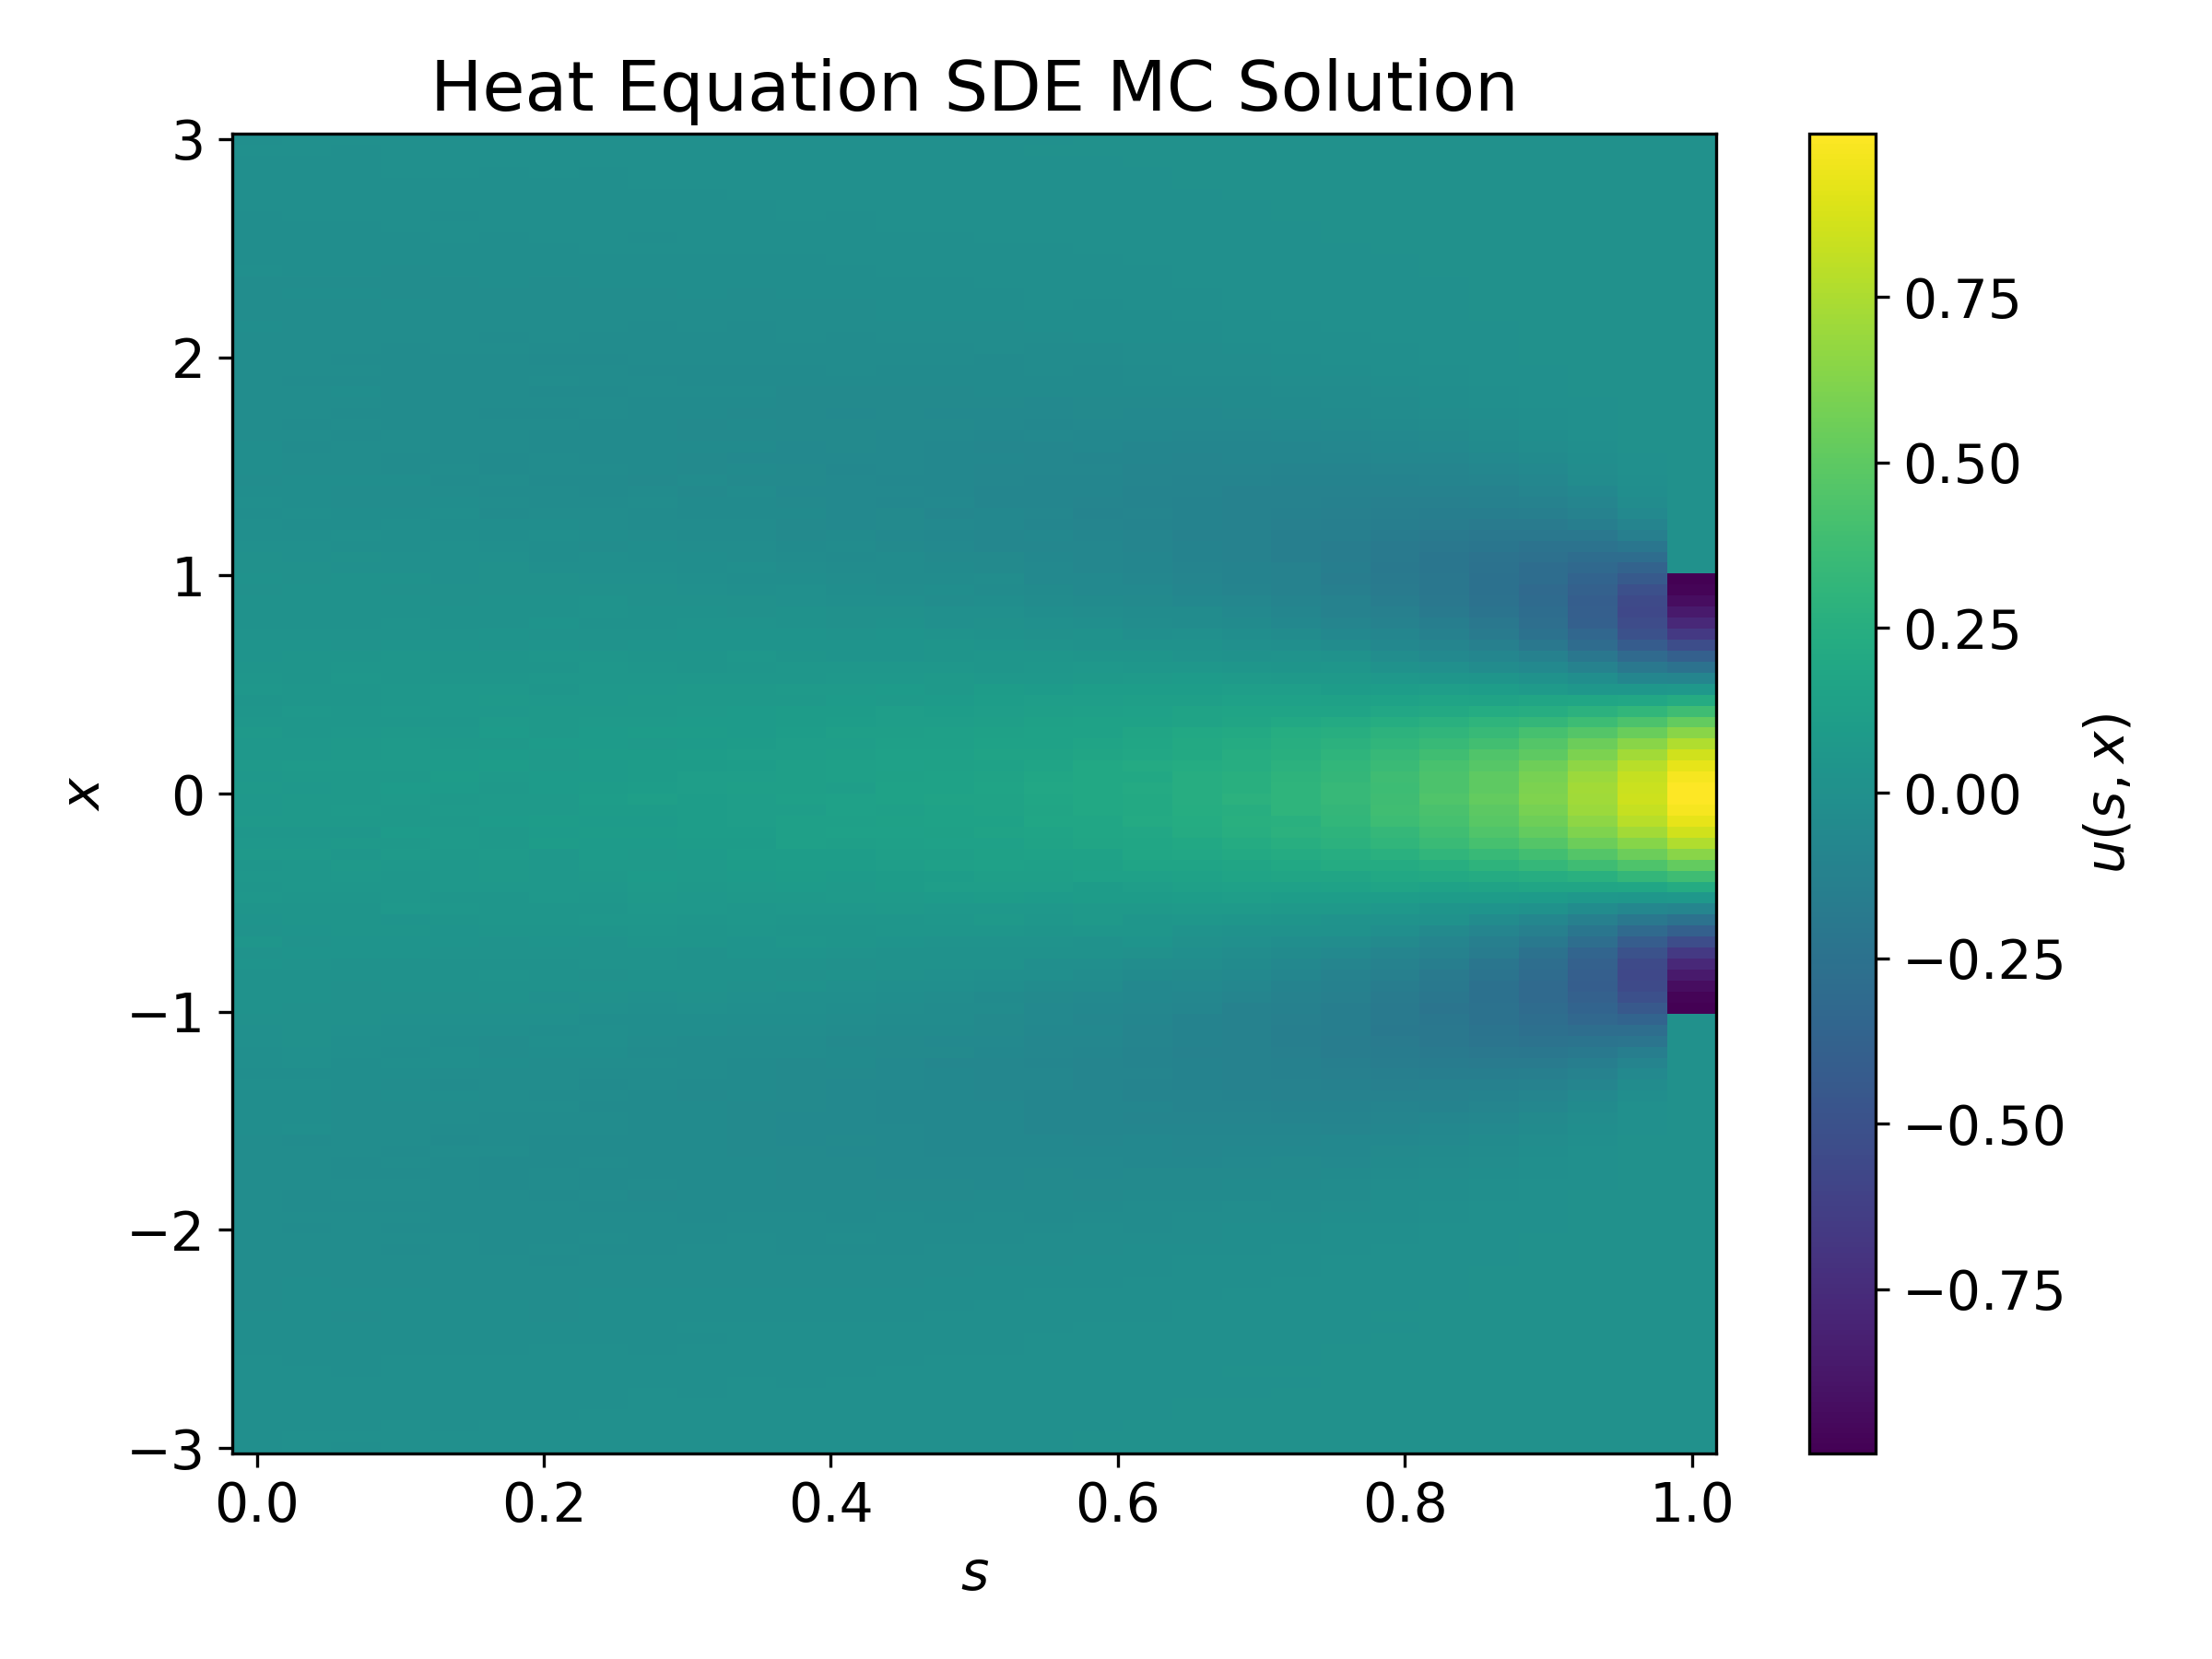
\includegraphics[width=\textwidth]{figures/Heat equation SDE MC Solution.jpg}
	\end{subfigure}
	\hfill
	\begin{subfigure}[b]{0.45\textwidth}
		\centering
		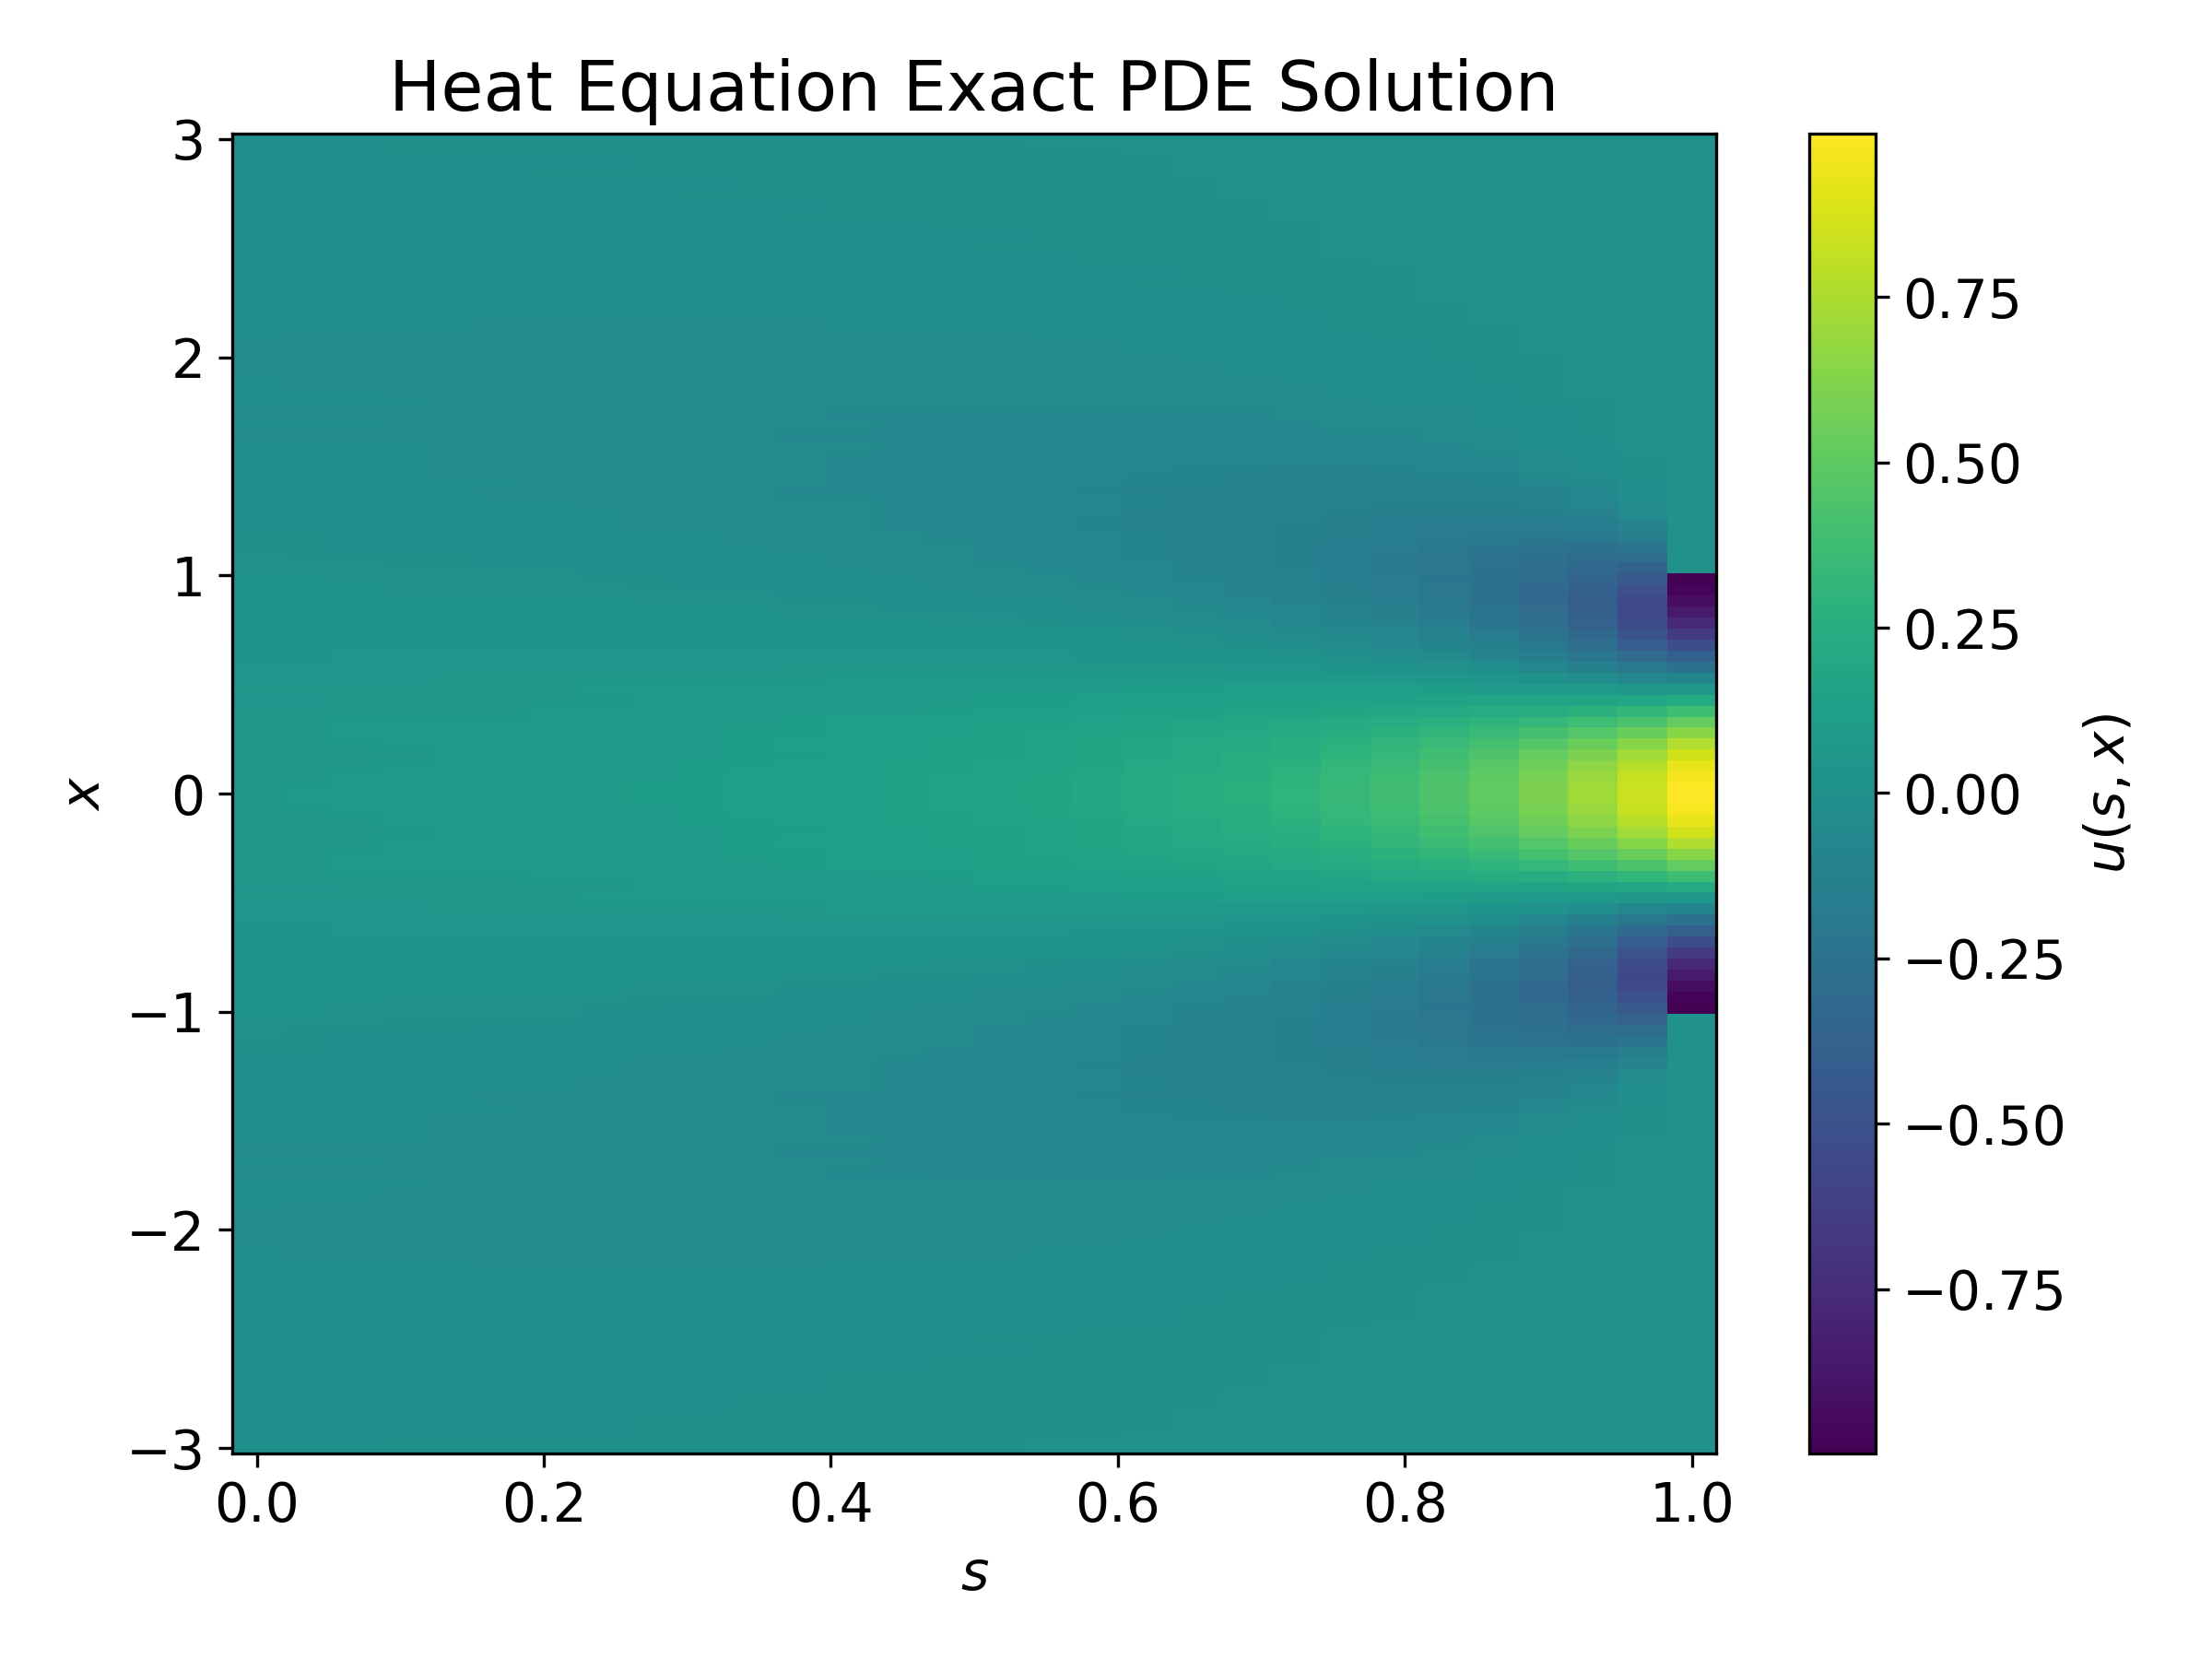
\includegraphics[width=\textwidth]{figures/Heat equation Exact PDE Solution.jpg}
	\end{subfigure}
	\caption{热方程SDE Monte Carlo求解（左）与PDE精确解（右）}
	\label{fig:3.6}
\end{figure}

图\ref{fig:3.7}（右）展示了SDE Monte Carlo方法在求解热方程上的实际收敛速率与理论收敛速率对比，从图上可以明显的看出实际收敛速率与理论收敛速率基本一致。因此若想进一步缩小误差，只需增大离散化区间数$N$与Monte Carlo路径数$M$即可。

\begin{figure}[htbp]
	\centering
	\begin{subfigure}[b]{0.45\textwidth}
		\centering
		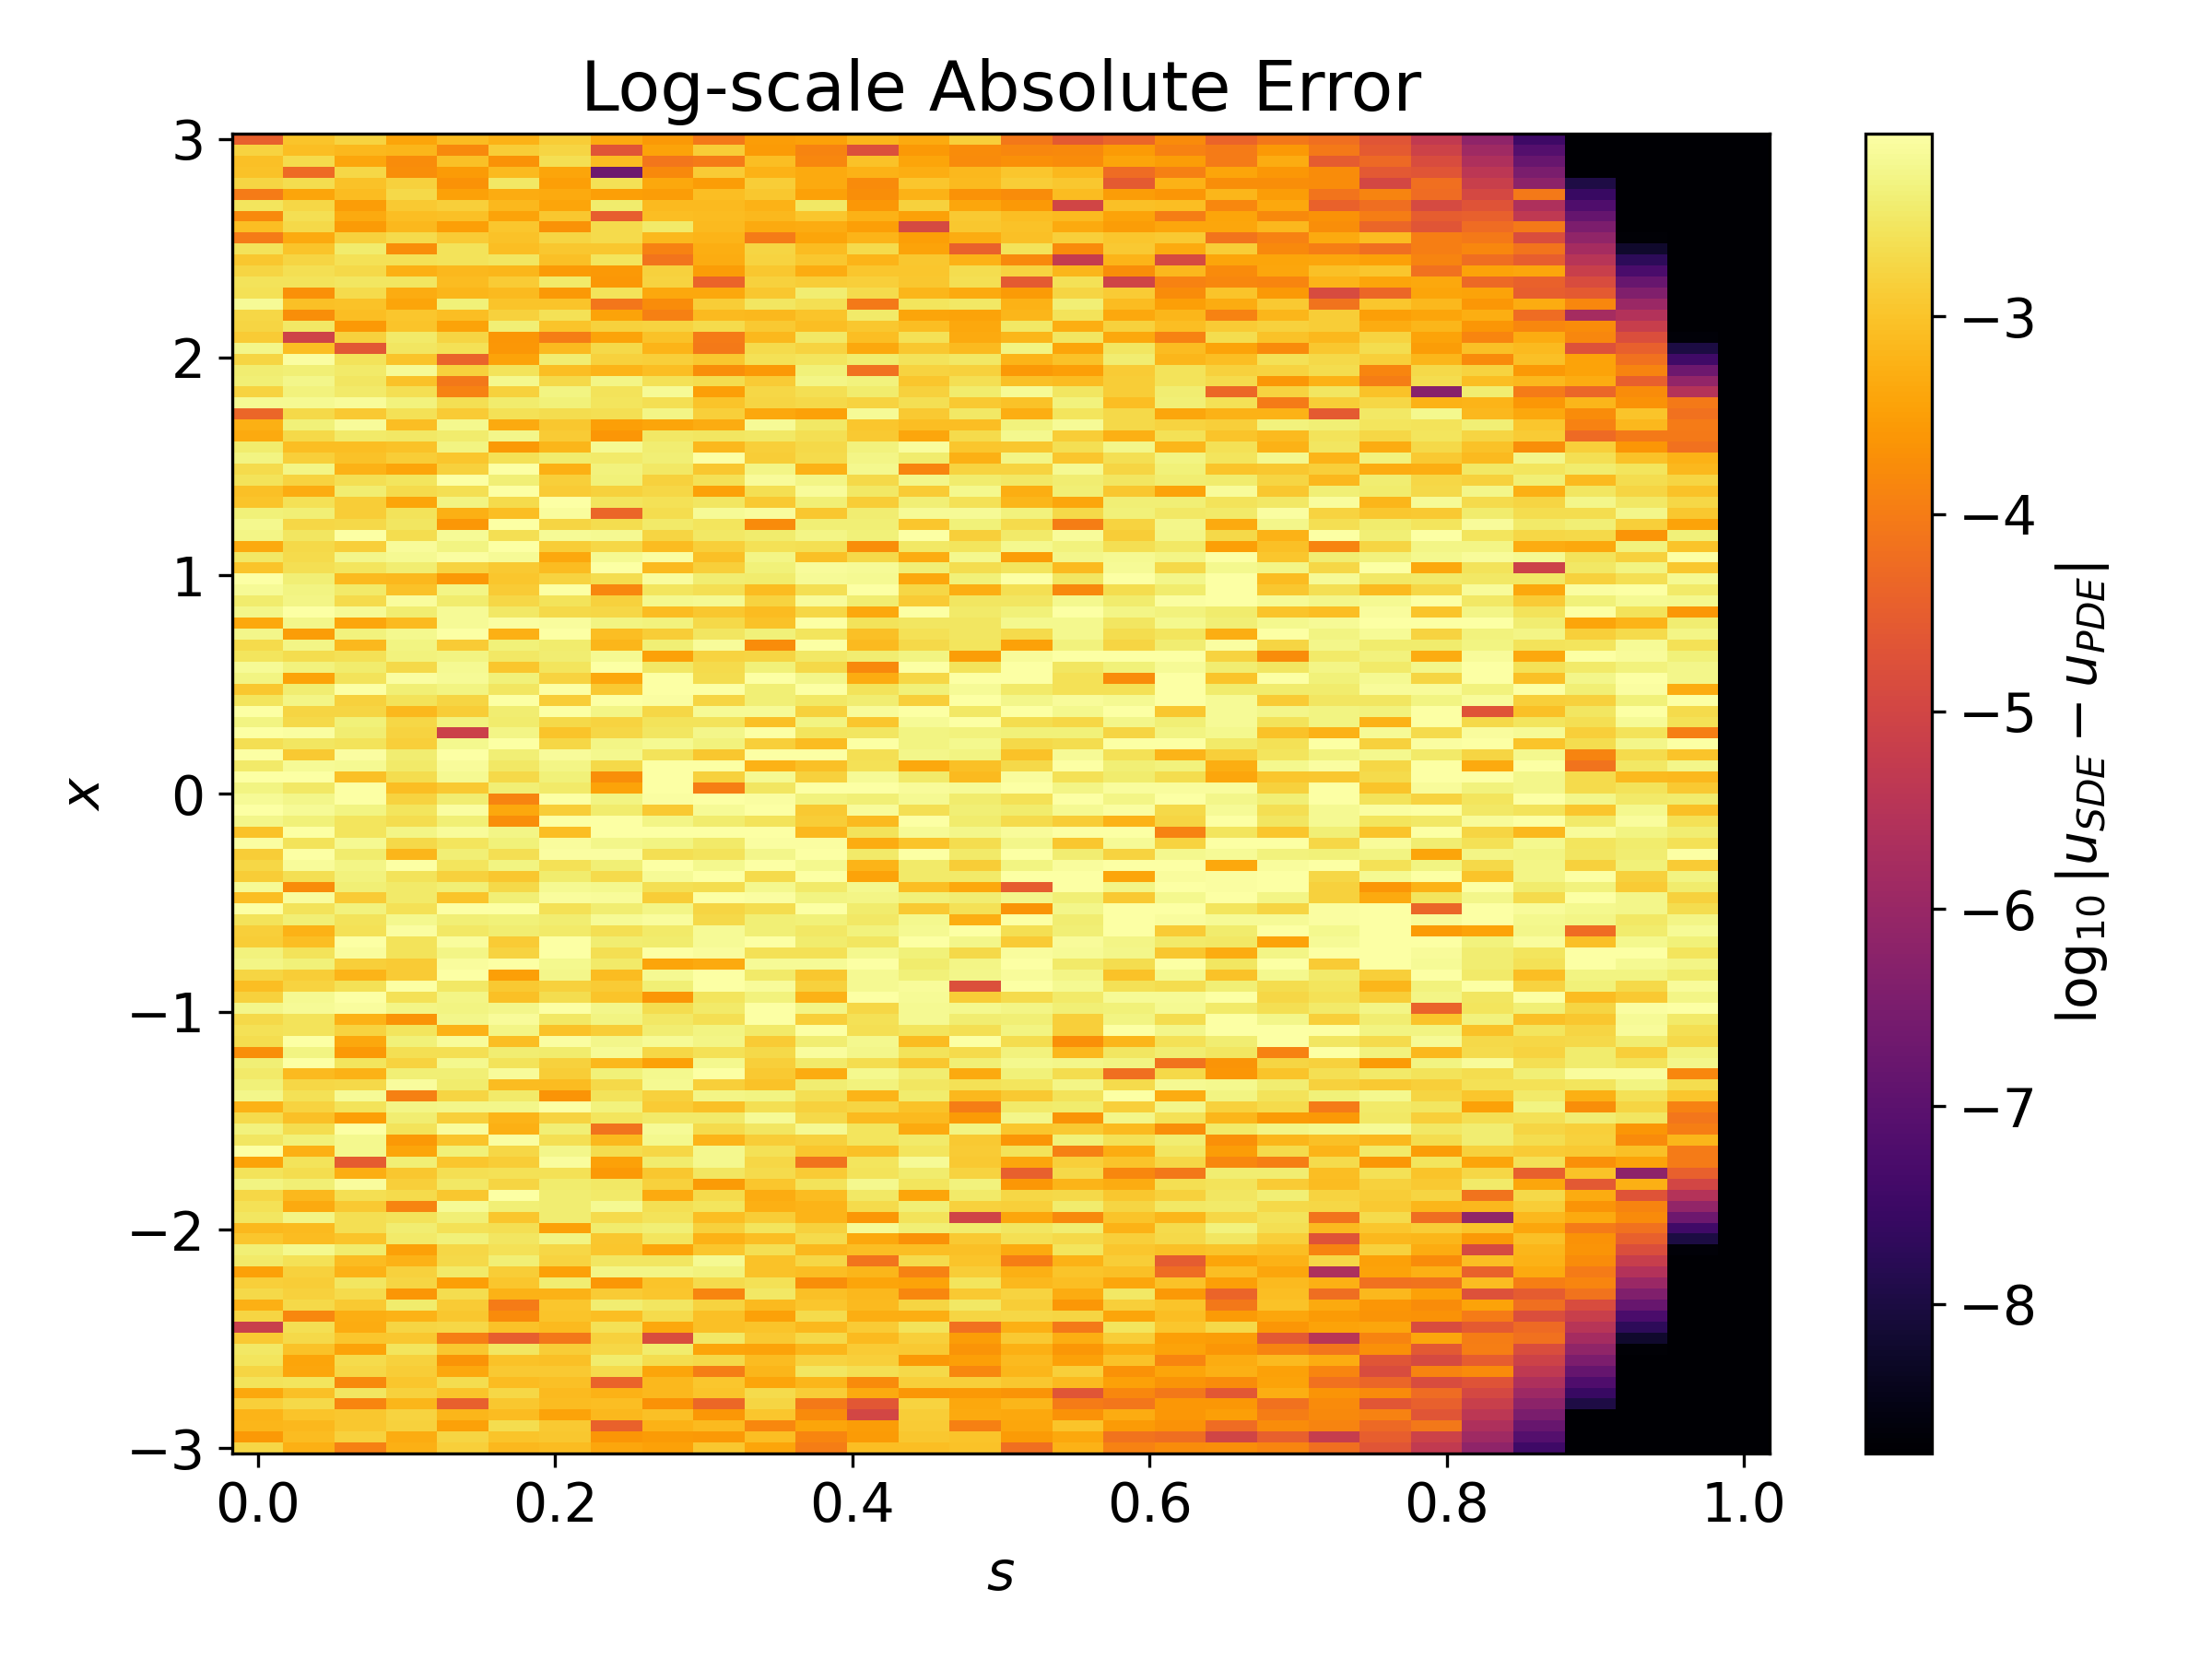
\includegraphics[width=\textwidth]{figures/Heat equation error.png}
	\end{subfigure}
	\hfill
	\begin{subfigure}[b]{0.45\textwidth}
		\centering
		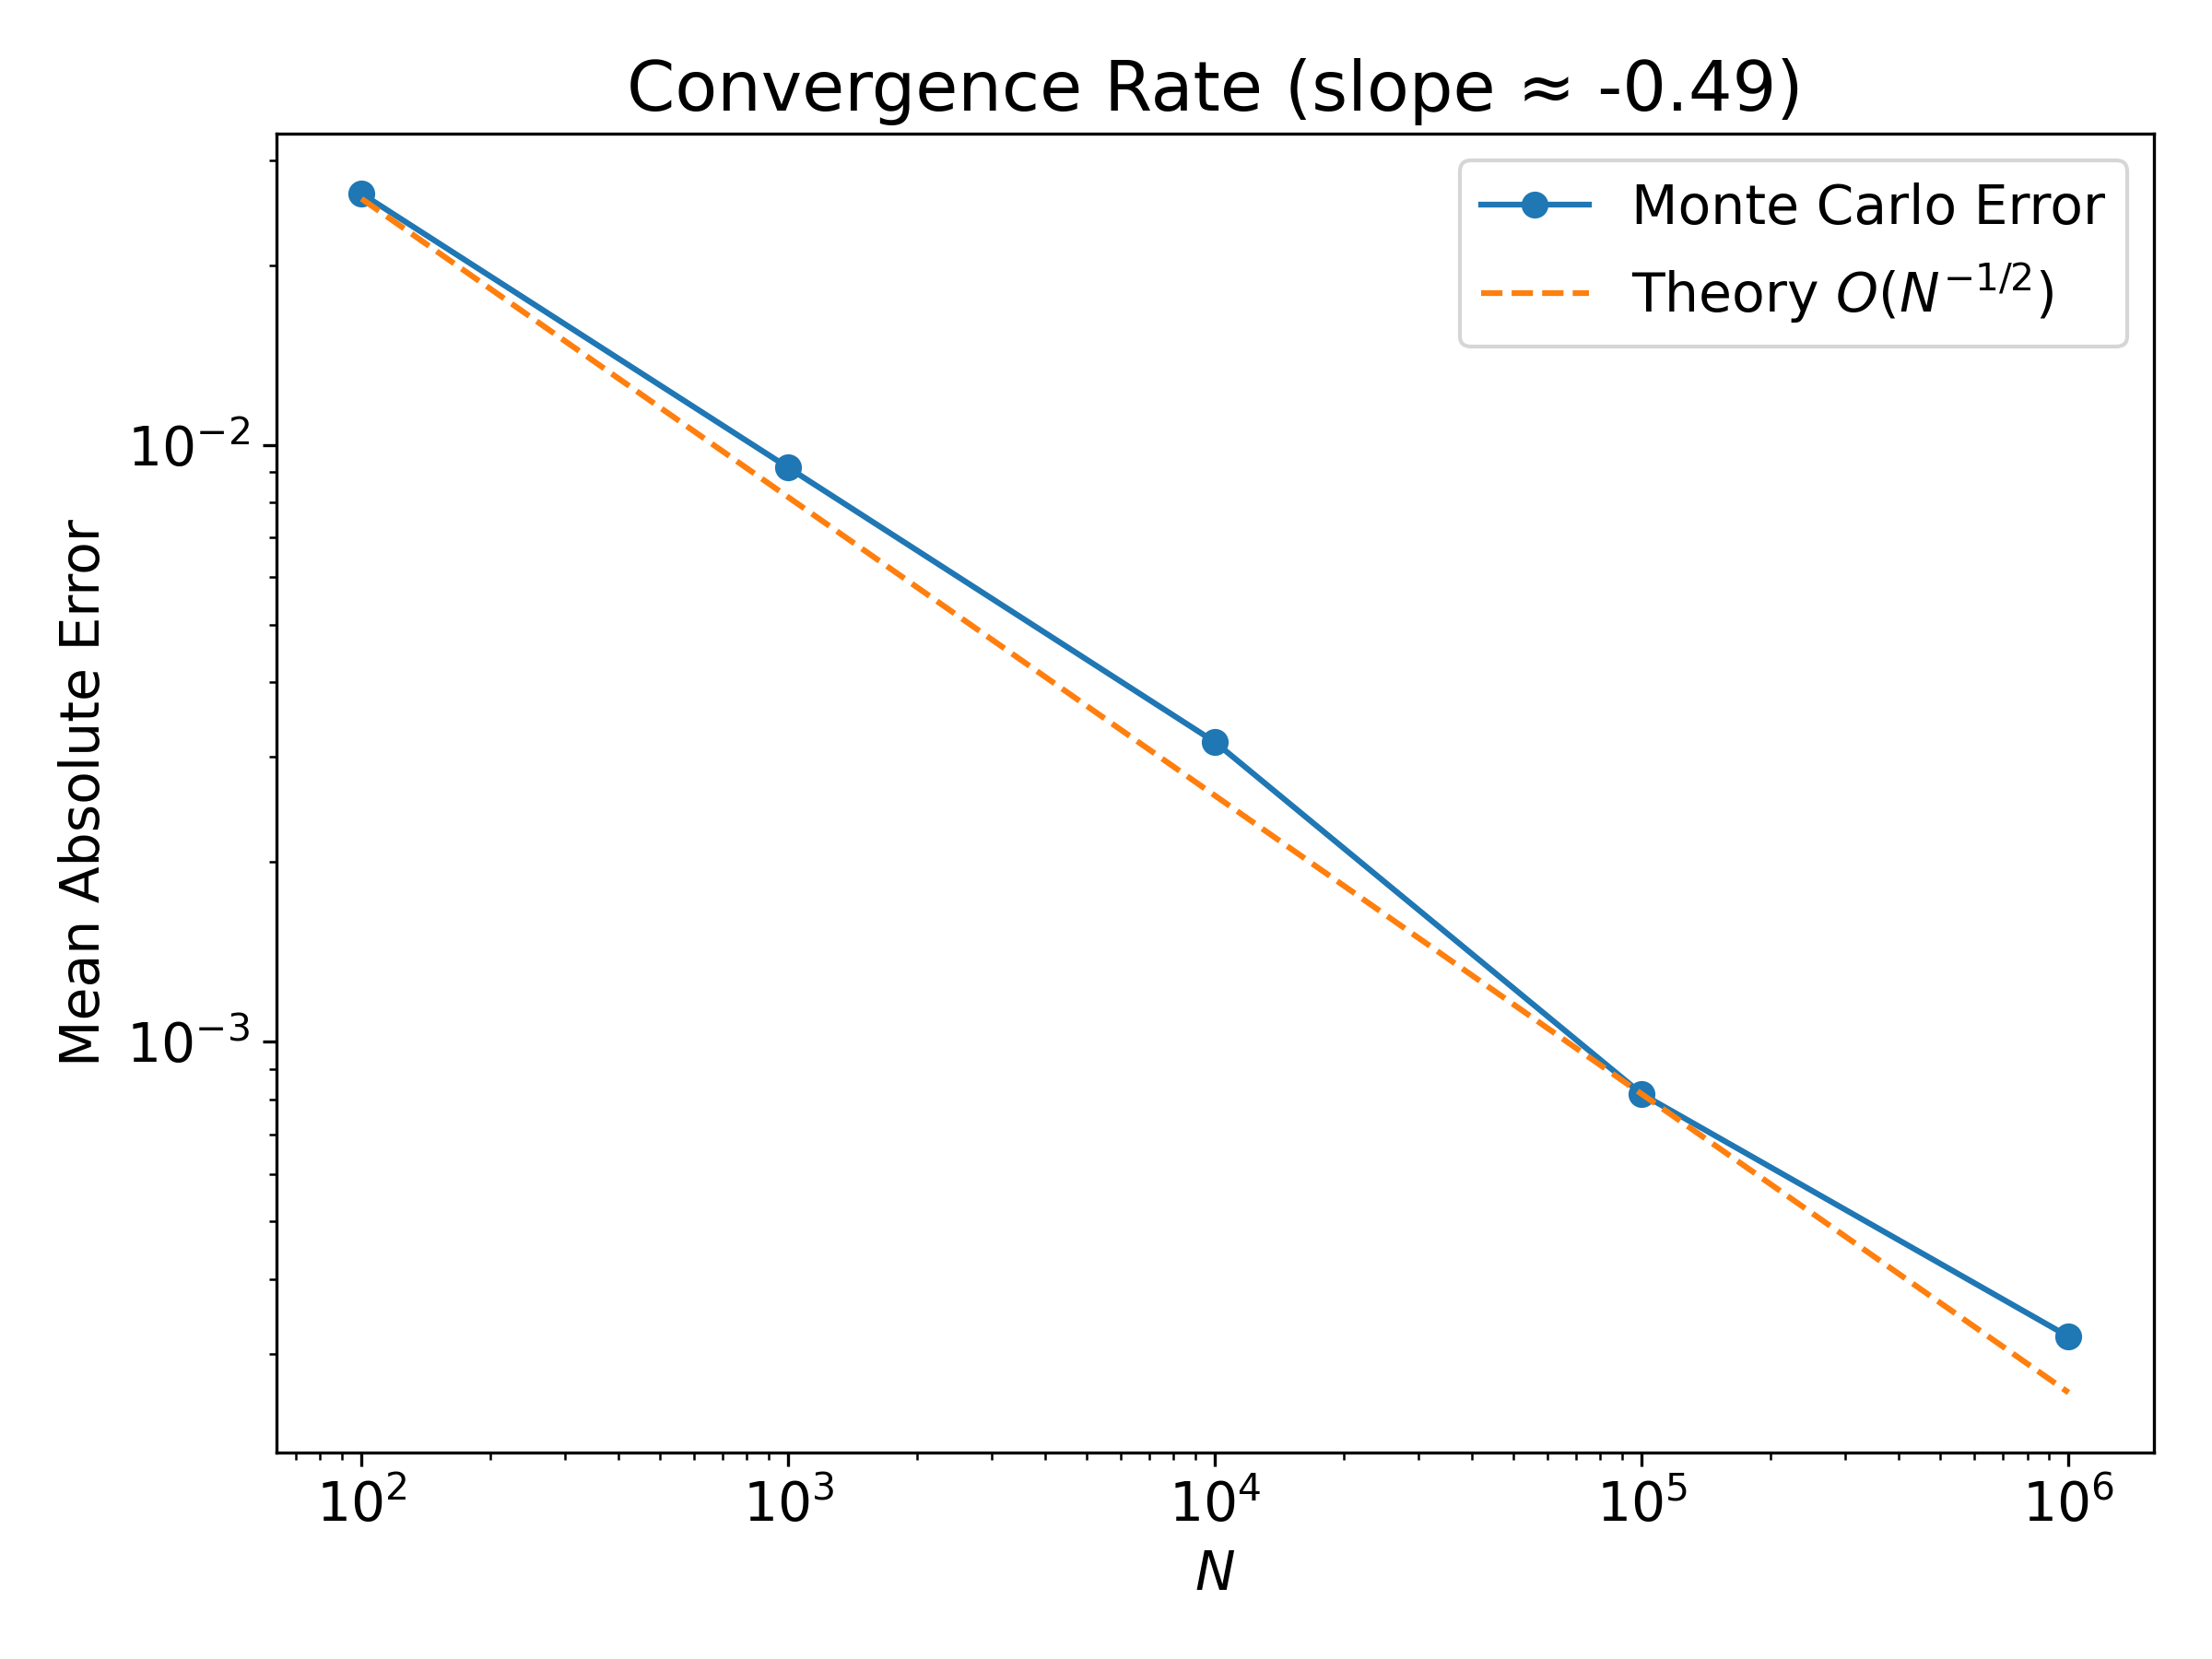
\includegraphics[width=\textwidth]{figures/Heat equation convergence rate.png}
	\end{subfigure}
	\caption{热方程SDE Monte Carlo解对数误差（左）与实际收敛速率 VS 理论收敛速率（右）}
	\label{fig:3.7}
\end{figure}

\newpage

\chapter{SDE在求解Black-Scholes方程中的应用}\label{chap:Black-Scholes}

本章主要介绍了Black-Scholes方程的背景、其经典PDE求解、利用Feynman-Kac公式的SDE方法求解、以及利用SDE Monte Carlo数值方法求解Black-Scholes方程。

\section{Black-Scholes方程背景}

期权定价长期以来是金融理论中的难题。早在1900年，法国数学家Louis Bachelier在其博士论文中首次尝试运用Brownian运动描述股票价格波动\cite{Bachelier2006}，并提出早期期权定价模型，它被公认为是现代金融学的里程碑。

1965年Paul Samuelson对L.Bcahelier的模型进行了修正\cite{Samuelson1965}，用股票的回报替代了原模型中的股票价格，这个修改克服了原先模型中可能使股票价格出现负值的不合理现象。后续几年里，随着资本资产定价模型（CAPM）思想\cite{sharpe1964capm}的提出，期权定价方法得到了重大改进，为后续突破奠定基础。

1968年前后，Fisher Black与Myron Scholes在麻省理工学院开始合作。F.Black最初尝试将CAPM应用于瞬间投资组合，发现通过动态调整持仓可消除风险，从而推导出一个不依赖标的资产期望回报率$\mu$的偏微分方程。同一时间，Robert C.Merton几乎同时独立开展相关研究，并对模型的数学基础进行了严谨拓展。他们共同提出了"Black-Scholes期权定价模型"这一名称\cite{BlackScholes1973}，三位学者的合作标志着量化金融时代的开端。

Black-Scholes模型的核心创新在于动态对冲与风险中性定价思想，通过构建适当的投资组合可以消除期权中的随机风险，从而在无套利条件下推导出期权价格必须满足的PDE。这一思路不仅解决了长期困扰的定价难题，还为后续风险管理提供了理论工具。

为了严格推导Black-Scholes方程，给出如下的基本假设：
\begin{equation*}
	dS_t=\mu S_tdt+\sigma S_tdB_t\,.
\end{equation*}
其中$\mu$为期望回报率，$\sigma$为波动率，均为$\mathbb{R}$中常数。$B_t$为一维标准Brownian运动。另还需无风险利率$r$为常数、原生资产不支付股息、不支付交易费和税收以及不存在套利机会的假设\cite{BlackScholes1973}。

设欧式期权价值为$V=V(S,t)$,由定理\ref{theo:multi_Ito_formula}，其瞬时变化为

\begin{equation}\label{equa:4.1}
	dV=\bigg(\frac{\partial V}{\partial t}+\mu S\frac{\partial V}{\partial S}+\frac{1}{2}\sigma^2 S^2\frac{\partial^2 V}{\partial S^2}\bigg)dt
	+\sigma S\frac{\partial V}{\partial S}dB_t\,.
\end{equation}
为消除风险，利用$\Delta-$对冲技巧\cite{hull2018}，形成投资组合
\begin{equation*}
	\Pi=V-\Delta S\,.
\end{equation*}
其中$\Delta$为原生资产的份额。选组适当的$\Delta$使得在$(t,t+dt)$时段内，$\Pi$是无风险的，从而在时刻$t+dt$，投资组合的回报是
\begin{equation*}
	\frac{\Pi_{t+dt}-\Pi_t}{\Pi_t}=rdt\,.
\end{equation*}
即
\begin{equation}\label{equa:4.2}
	dV_t-\Delta dS_t=r\Pi_t dt=r(V_t-\Delta S_t)dt\,.
\end{equation}
结合式\eqref{equa:4.1}，将其带入式\eqref{equa:4.2}得
\begin{equation}\label{equa:4.3}
	\begin{split}
		\bigg(\frac{\partial V}{\partial t}+\mu S\frac{\partial V}{\partial S}+\frac{1}{2}\sigma^2 S^2&\frac{\partial^2 V}{\partial S^2}-\Delta\mu S\bigg)dt+\bigg(\sigma S\frac{\partial V}{\partial S}-\Delta\sigma S\bigg)dB_t\\
		&=r(V-\Delta S)dt.
	\end{split}
\end{equation}
由于等式右端是无风险的，因此等式左端随机项$dB_t$的系数必为0，即选取
\begin{equation*}
	\Delta=\frac{\partial V}{\partial S}\,.
\end{equation*}
将其回代回式\eqref{equa:4.3}得
\begin{equation}
	\frac{\partial V}{\partial t}+\frac{1}{2}\sigma^2 S^2\frac{\partial^2 V}{\partial S^2}+rS\frac{\partial V}{\partial S}-rV=0\,.
\end{equation}
就得到了刻画期权价格变化的偏微分方程--Black-Scholes方程。

为了确定在合约有效期$[0,T]$内期权的价格，就要在区域$D$上求解定解问题：
\[
\begin{cases}
	\dfrac{\partial V}{\partial t} + \dfrac{1}{2}\sigma^2 S^2 \dfrac{\partial^2 V}{\partial S^2} + rS \dfrac{\partial V}{\partial S} - rV = 0\,, & (S,t)\in D.\\[10pt]
	V|_{t=T} = 
	\begin{cases}
		(S - K)^+, & \text{(欧式看涨期权)} \\
		(K - S)^+, & \text{(欧式看跌期权)}
	\end{cases}
\end{cases}
\]
其中$K$为期权的敲定价，区域$D:=\left\{0<S<\infty,0<t<T\right\}$。易知上述偏微分方程是一变系数反抛物型方程，并为一倒向定解问题：即在终止时间已知"终值条件"，在$0<t<T$时段内求解$V=V(S,t)$,使其满足上述偏微分方程和终止条件。

值得注意的是，在Black-Scholes方程中，并未包含原生资产模型中该资产的期望回报率$\mu$,取而代之的是无风险利率$r$。这表明通过$\Delta-$对冲策略，Black-Scholes方程将期权定价置于一个风险中性测度之下。其定价结果独立于投资者的风险偏好，以及他们对风险资产未来回报的任何主观预期。因此，通过求解Black-Scholes方程得到的期权价格，本质上是在风险中性测度下所得到的公平价格。

\section{Black-Scholes方程的经典PDE求解}

可作变换
\begin{equation*}
	x=ln S,\hspace{0.3cm}h=T-t.
\end{equation*}
则原定解问题转化为常系数抛物型方程的Cauchy问题：
\[
\begin{cases}
	\dfrac{\partial V}{\partial h} - \dfrac{1}{2}\sigma^2 \dfrac{\partial^2 V}{\partial x^2} - (r-\dfrac{\sigma^2}{2})\dfrac{\partial V}{\partial x}+rV = 0\,, & (x,h)\in (-\infty,\infty)\times(0,T)\,.\\[10pt]
	V|_{h=0} = 
	\begin{cases}
		(e^x - K)^+, & \text{(看涨期权)} \\
		(K - e^x)^+, & \text{(看跌期权)}
	\end{cases}
\end{cases}
\]

做函数变换
\begin{equation*}
	V=ue^{\alpha h+\beta x}.
\end{equation*}
可通过适当选取常数$\alpha,\beta$使得上述偏微分方程转化为热传导方程。由于
\begin{equation*}
	\begin{split}
		&V_h=e^{\alpha h+\beta x}(u_h+\alpha u),\\
		&V_x=e^{\alpha h+\beta x}(u_x+\beta u),\\
		&V_{xx}=e^{\alpha h+\beta x}(u_xx+2\beta u_x+\beta^2 u).\\
	\end{split}
\end{equation*}
将其带入方程，消去$e^{\alpha h+\beta x}$得到
\begin{equation*}
	u_h-\dfrac{\sigma^2}{2}u_{xx}-(\beta\sigma^2+r-\frac{\sigma^2}{2})u_x+\\\left[r-\beta(r-\dfrac{\sigma^2}{2})-\dfrac{\sigma^2}{2}\beta^2+\alpha\right]u=0\,.
\end{equation*}
取
\begin{equation}\label{equa:4.5}
	\begin{split}
		&\beta=\dfrac{1}{2}-\dfrac{r}{\sigma^2}\\
		&\alpha=-r+\beta(r-\dfrac{\sigma^2}{2})+\dfrac{\sigma^2}{2}\beta^2=-r-\dfrac{1}{2\sigma^2}(r-\dfrac{\sigma^2}{2})^2.\\
	\end{split}
\end{equation}
从而原方程变为
\begin{equation*}
	\dfrac{\partial u}{\partial h}-\dfrac{\sigma^2}{2}\dfrac{\partial^2 u}{\partial x^2}=0\,.
\end{equation*}
相应的初值（以看涨期权为例）为
\begin{equation*}
	u|_{h=0}=e^{-\beta x}V|_{h=0}=e^{-\beta x}(e^x-K)^+.
\end{equation*}

而上述热方程的Cauchy问题的解可以用Poisson公式表示\cite{evans2010pde}，即
\begin{equation*}
	u(x,h)=\int_{-\infty}^{+\infty}K(x-\xi,h)\phi(\xi)d\xi.
\end{equation*}
其中$\phi(\xi)$为初值，$K(x-\xi,h)$为热方程的基本解：
\begin{equation*}
	K(x-\xi,h)=\dfrac{1}{\sigma\sqrt{2\pi h}}e^{-\frac{(x-\xi)^2}{2\sigma^2 h}}\,.
\end{equation*}
从而上述看涨期权初值的Cauchy问题的解可以表示为
\begin{equation*}
	\begin{split}
		u(x,h)&=\int_{-\infty}^{+\infty}\dfrac{1}{\sigma\sqrt{2\pi h}}e^{-\frac{(x-\xi)^2}{2\sigma^2 h}}\left[e^{-\beta\xi}(e^\xi-K)^+\right]d\xi\\
		&=\int_{\ln K}^{+\infty}\dfrac{1}{\sigma\sqrt{2\pi h}}e^{-\frac{(x-\xi)^2}{2\sigma^2 h}}\left[e^{(1-\beta)\xi}-Ke^{-\beta\xi}\right]d\xi\,.
	\end{split}
\end{equation*}
其中$\beta=\dfrac{1}{2}-\dfrac{r}{\sigma^2}$。回到原来的函数$V(x,h)$
\begin{equation*}
	\begin{split}
		V(x,h)&=e^{\alpha h+\beta x}u(x,h)\\
		&=I_1+I_2.\\
	\end{split}
\end{equation*}
其中
\begin{equation}\label{equa:4.6}
	I_1=e^{\alpha h+\beta x}\int_{\ln K}^{+\infty}\dfrac{1}{\sigma\sqrt{2\pi h}}e^{-\frac{(x-\xi)^2}{2\sigma^2 h}+(1-\beta)\xi}.
\end{equation}
将式\ref{equa:4.5}带入式\ref{equa:4.6}并整理得：
\begin{equation*}
	I_1=e^{-rh}\int_{\ln K}^{\infty}\dfrac{1}{\sigma\sqrt{2\pi h}}\exp\left\{-\dfrac{1}{2\sigma^2 h}\left[x-\xi+(r-\dfrac{\sigma^2}{2})h\right]^2+\xi\right\}d\xi\,.
\end{equation*}
令
\begin{equation*}
	\eta=x-\xi+(r-\dfrac{\sigma^2}{2})h.
\end{equation*}
则
\begin{equation*}
	I_1=\dfrac{e^x}{\sigma\sqrt{2\pi h}}\int_{-\infty}^{x-\ln K+(r-\frac{\sigma^2}{2})h}e^{-\frac{(\eta+\sigma^2h)^2}{2\sigma^2 h}}d\eta\,.
\end{equation*}
再令
\begin{equation*}
	\omega=\dfrac{\eta+\sigma^2 h}{\sigma\sqrt{h}},\hspace{0.3cm}\Phi(x)=\dfrac{1}{\sqrt{2\pi}}\int_{-\infty}^{x}e^{-\frac{\omega^2}{2}}d\omega\,.
\end{equation*}
即$\Phi(x)$为标准正态分布得累积概率分布函数，从而$I_1$可写成
\begin{equation*}
	I_1=e^x\Phi\Bigg(\dfrac{x-\ln K+(r+\frac{\sigma^2}{2})h}{\sigma\sqrt{h}}\Bigg).
\end{equation*}

同理
\begin{equation*}
	\begin{split}
		I_2&=-Ke^{\alpha h+\beta x}\int_{\ln K}^{+\infty}\dfrac{1}{\sigma\sqrt{2\pi h}}e^{-\frac{(x-\xi)^2}{2\sigma^2 h}-\beta\xi}\\
		&=-e^{-rh}\int_{\ln K}^{+\infty}\dfrac{K}{\sigma\sqrt{2\pi h}}e^{-\frac{1}{2\sigma^2 h}\left[x-\xi+(r-\frac{\sigma^2}{2})h\right]^2}d\xi\\
		&=-\dfrac{e^{-rh}K}{\sigma\sqrt{2\pi h}}\int_{-\infty}^{x-\ln K+(r-\frac{\sigma^2}{2})h}e^{-\frac{\eta^2}{2\sigma^2 h}}d\eta\\
		&=-Ke^{-rh}\Phi\Big(\dfrac{x-\ln K+(r-\frac{\sigma^2}{2})h}{\sigma\sqrt{h}}\Big).\\
	\end{split}
\end{equation*}

回到原变量$(S,t)$，有
\begin{equation*}
	\begin{split}
		V(S,t)=&S\Phi\Big(\dfrac{\ln S-\ln K+(r+\frac{\sigma^2}{2})(T-t)}{\sigma\sqrt{T-t}}\Big)\\
		&-Ke^{-r(T-t)}\Phi\Big(\dfrac{\ln S-\ln K+(r-\frac{\sigma^2}{2})(T-t)}{\sigma\sqrt{T-t}}\Big).\\
	\end{split}
\end{equation*}
令
\begin{equation*}
	\begin{split}
		d_1&=\dfrac{\ln S-\ln K+(r+\frac{\sigma^2}{2})(T-t)}{\sigma\sqrt{T-t}},\\
		d_2&=d_1-\sigma\sqrt{T-t}.
	\end{split}
\end{equation*}
从而对欧式看涨期权，它的定价公式为
\begin{equation*}
	V(S,t)=S\Phi(d_1)-Ke^{-r(T-t)}\Phi(d_2).
\end{equation*}

对于欧式看跌期权，由平价公式\cite{hull2018}
\begin{equation*}
	c_t+Ke^{-r(T-t)}=p_t+S_t\,.
\end{equation*}
其中$c_t$为欧式看涨期权，$p_t$为欧式看跌期权。
从而
\begin{equation*}
	\begin{split}
		p_t=c_t+Ke^{-r(T-t)}-S_t&=Ke{-r(T-t)}\left[1-\Phi(d_2)\right]-S\left[1-\Phi(d_1)\right]\\
		&=Ke^{-r(T-t)}\Phi(-d_2)-S\Phi(d_1).\\
	\end{split}
\end{equation*}
即欧式看跌期权的定价公式为
\begin{equation*}
	V(S,t)=Ke^{-r(T-t)}\Phi(-d_2)-S\Phi(d_1).
\end{equation*}

\section{Black-Scholes方程的SDE方法求解}

以欧式看涨期权为例，先将问题重述一遍。设区域$D:\left\{0<S<\infty,0<t<T\right\}$，求解以下定解问题。
\[
\begin{cases}
	\dfrac{\partial V}{\partial t} + \dfrac{1}{2}\sigma^2 S^2 \dfrac{\partial^2 V}{\partial S^2} + rS \dfrac{\partial V}{\partial S} - rV = 0\,, & (S,t)\in D\,.\\[10pt]
	V|_{t=T} = (S - K)^+.
\end{cases}
\]

令$h=T-t,U(S,h)=V(S,T-h)$，则由
\begin{equation*}
	\begin{split}
		&\dfrac{\partial U}{\partial h}=-\dfrac{\partial V}{\partial t},\quad
		\dfrac{\partial U}{\partial S}=\dfrac{\partial V}{\partial S},\quad
		\dfrac{\partial^2 U}{\partial S^2}=\dfrac{\partial^2 V}{\partial S^2}.
	\end{split}
\end{equation*}
变换后的微分方程为

\[
\begin{cases}
	rS\dfrac{\partial U}{\partial S}+\dfrac{1}{2}\sigma^2 S^2\dfrac{\partial^2 U}{\partial S^2}-rU=\dfrac{\partial U}{\partial h}\,, & (S,h)\in D\,.\\[10pt]
	U|_{h=0} = (S - K)^+.
\end{cases}
\]

记
\begin{equation*}
	L=rS\dfrac{\partial}{\partial S}+\dfrac{1}{2}\sigma^2 S^2\dfrac{\partial^2}{\partial S^2}.
\end{equation*}
为上述偏微分方程的偏微分算子。

设$X_t$为几何Brownian运动
\begin{equation*}
	dX_t=rX_tdt+\sigma X_tdB_t;\hspace{0.3cm}X_0=S.
\end{equation*}
而由定理\ref{theo:lemma_2}知，$X_t$的无穷小生成元恰好是$L$。因此定理\ref{theo:Feynman-Kac_formula}知上述偏微分方程的唯一解为
\begin{equation}
	\begin{split}
		U(S,h)&=\mathbb{E}^S\left[\exp(-\int_{0}^{h}rds)(X_h-K)^+\right]\\
		&=\mathbb{E}^S\left[e^{-rh}(X_h-K)^+\right].
	\end{split}
\end{equation}
再将变换代回得
\begin{equation}
	V(S,t)=\mathbb{E}^S\left[e^{-r(T-t)}(X_{T-t}-K)^+\right],\hspace{0.3cm}(S,t)\in D.
\end{equation}

对于欧式看跌期权，则同理可得到其定价公式为
\begin{equation}
	V(S,t)=\mathbb{E}^S\left[e^{-r(T-t)}(K-X_{T-t})^+\right],\hspace{0.3cm}(S,t)\in D.
\end{equation}
由此可以利用SDE Monte Carlo方法求解欧式看涨期权和欧式看跌期权下的Black-Scholes方程。

\section{SDE Monte Carlo数值方法求解Black-Scholes方程}

将Black-Scholes方程中各项系数分别取为
\begin{equation*}
	\begin{split}
		r&=0.025\,, \quad
		\sigma=0.2\,, \quad
		T=1.0\,, \quad
		K=1.0\,.
	\end{split}
\end{equation*}
并取离散化子区间数为$N=1000$（也即$\Delta t=0.001$），Monte Carlo样本数$M=10000$，在$S\in[0,3],t\in[0,1]$上利用SDE Monte Carlo方法求解Black-Scholes方程，并与PDE精确解进行对比。

图\ref{fig:4.1}与图\ref{fig:4.2}分别展示了在欧式看涨期权与欧式看跌期权初值条件下，Black-Scholes方程的SDE Monte Carlo解与PDE精确解。从两张结果图直观来看，无论是欧式看涨期权还是欧式看跌期权条件下，利用SDE Monte Carlo方法求得的数值解与PDE精确解相差无几。


而图\ref{fig:4.3}则直接具体分别展现了欧式看涨期权和欧式看跌期权条件下的二者的对数误差分布。根据图中的对数误差分布可以明显看出，在欧式看涨期权的初值条件下，大致在直线$S=0.5t+0.5$以下区域误差极低（小于$10^{-8}$），而在其上区域误差则相对较高，但也均在$10^{-3}$量级之内，通过计算得出的平均相对误差为$2.49\times 10^{-3}$；而相比于欧式看涨期权，欧式看跌期权初值条件下区域内的误差基本均处于$10^{-4}$量级，通过计算得出的平均相对误差为$5.32\times 10^{-4}$，且大致在$S=-1.75t+3$以下区域误差极低（小于$10^{-8}$）。

\begin{figure}[htbp]
	\centering
	\begin{subfigure}[b]{0.45\textwidth}
		\centering
		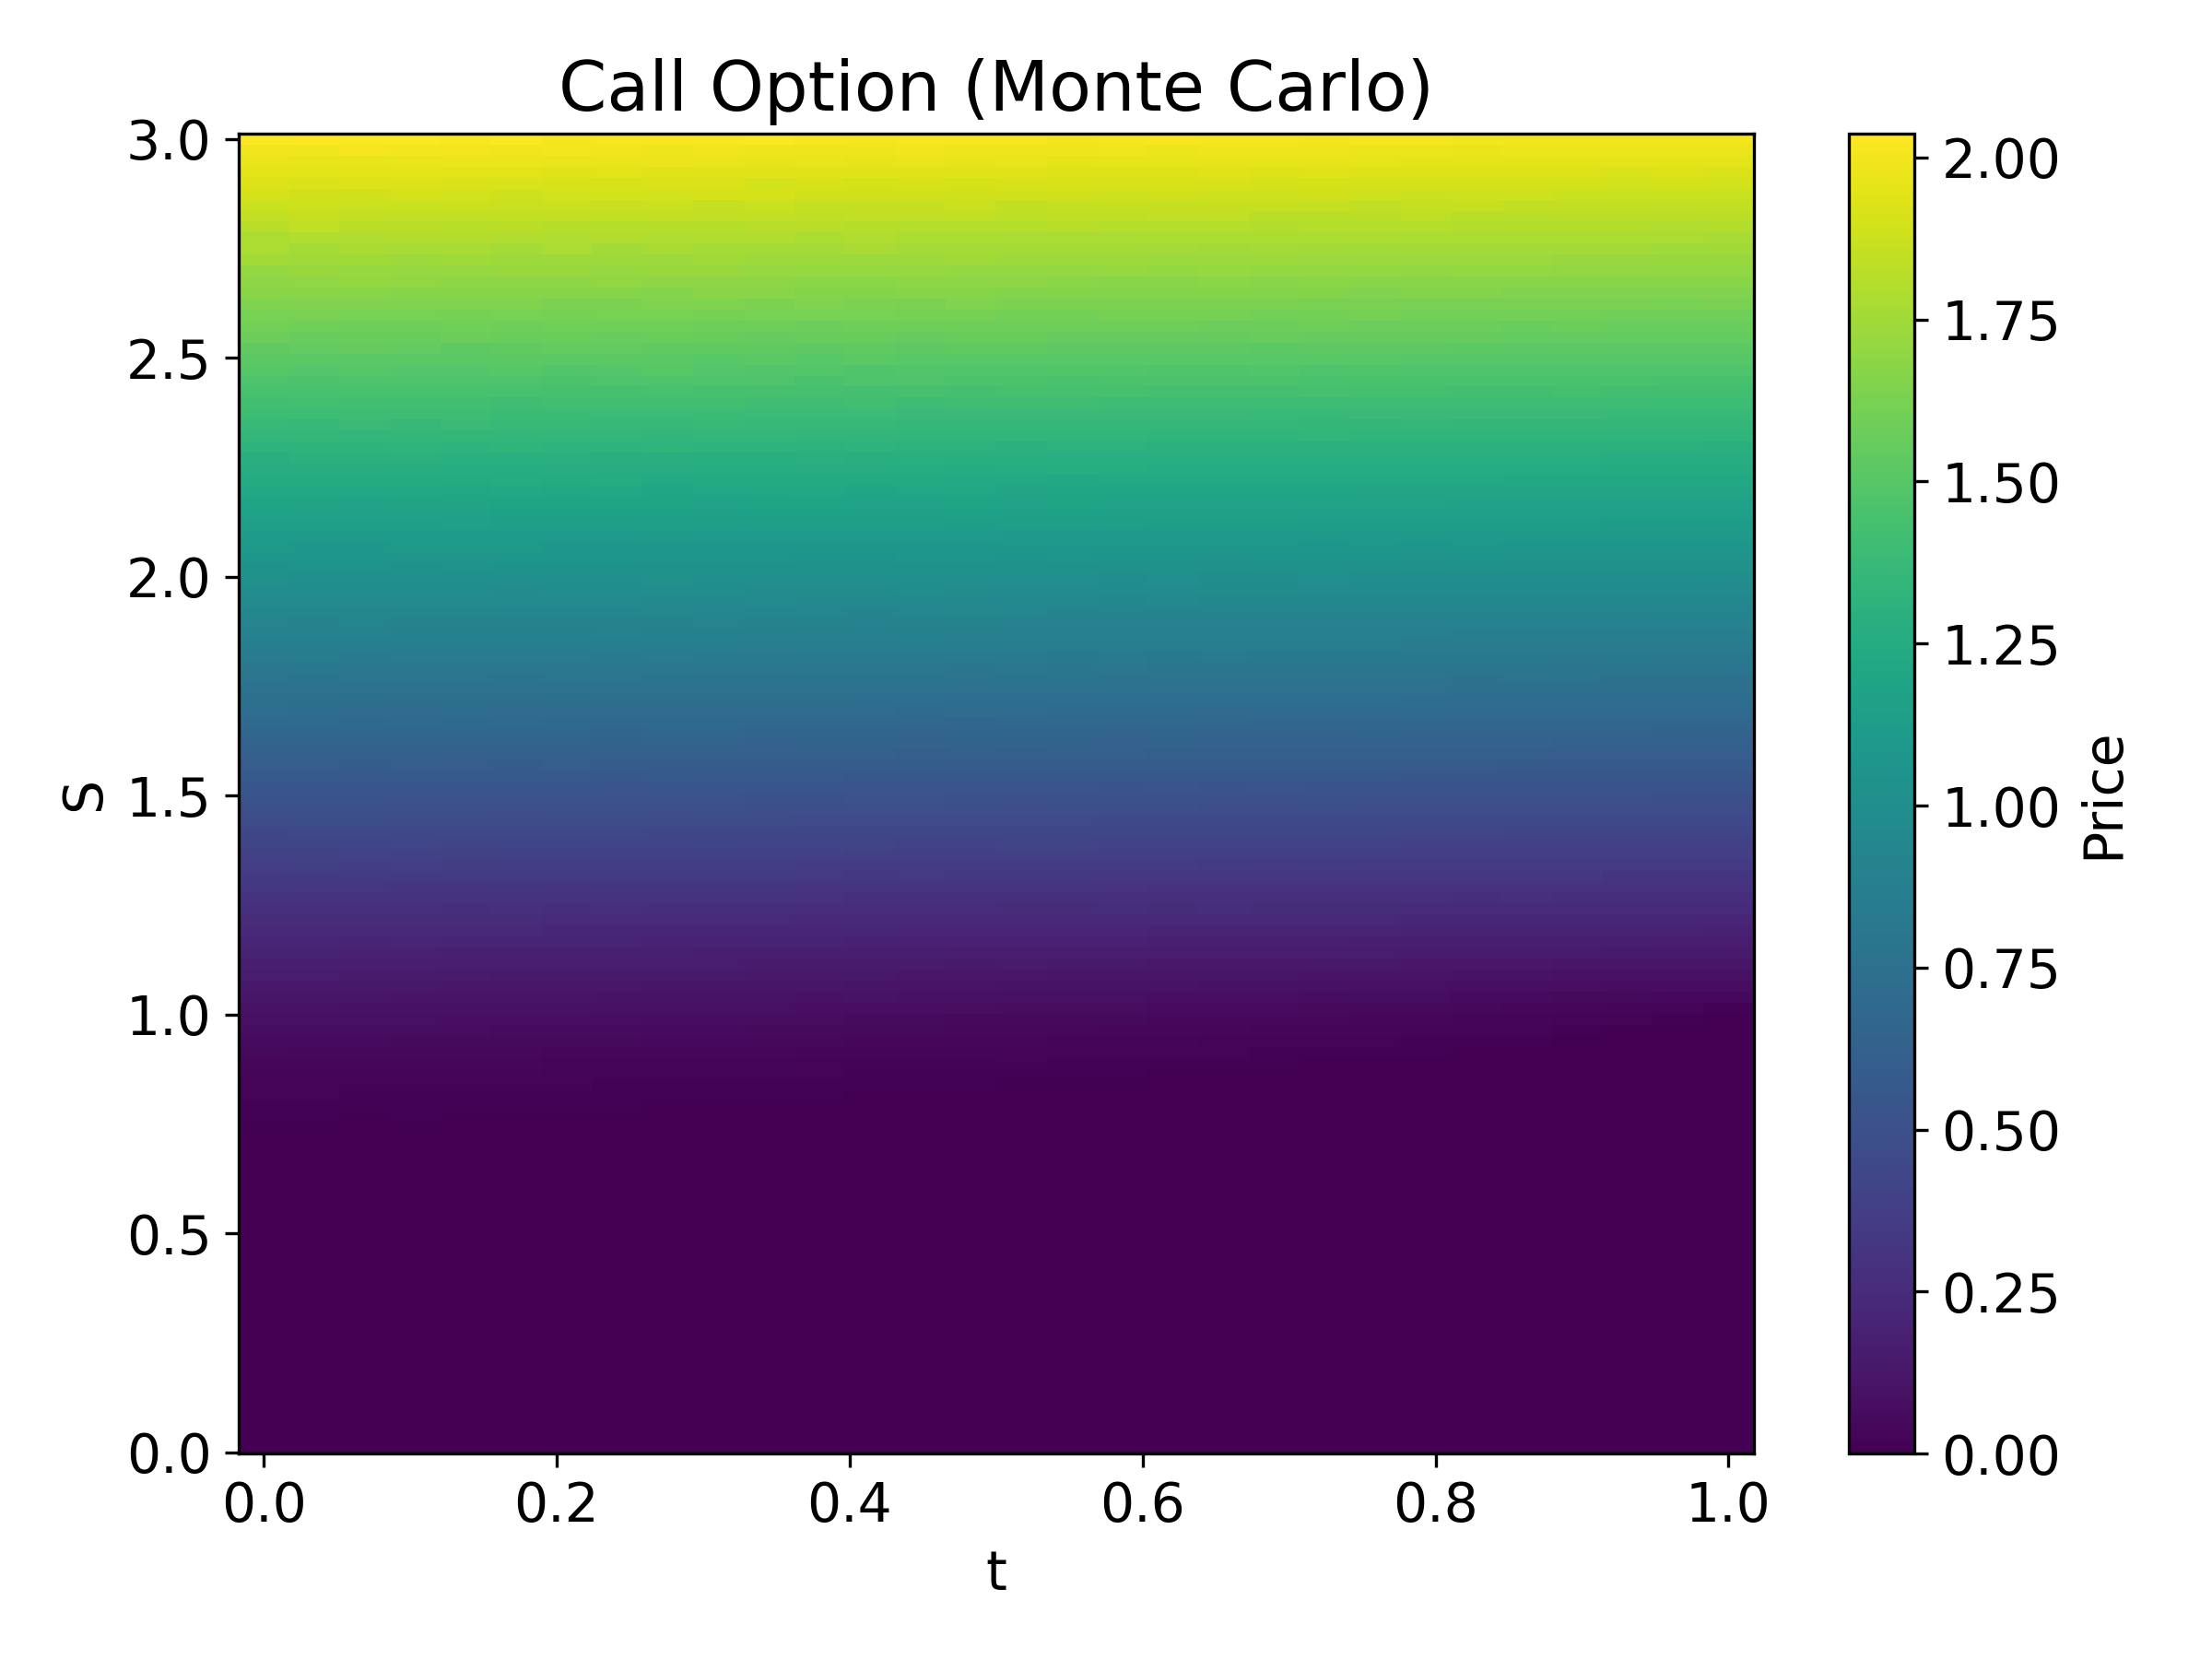
\includegraphics[width=\textwidth]{figures/call option MC solution.jpg}
	\end{subfigure}
	\hfill
	\begin{subfigure}[b]{0.45\textwidth}
		\centering
		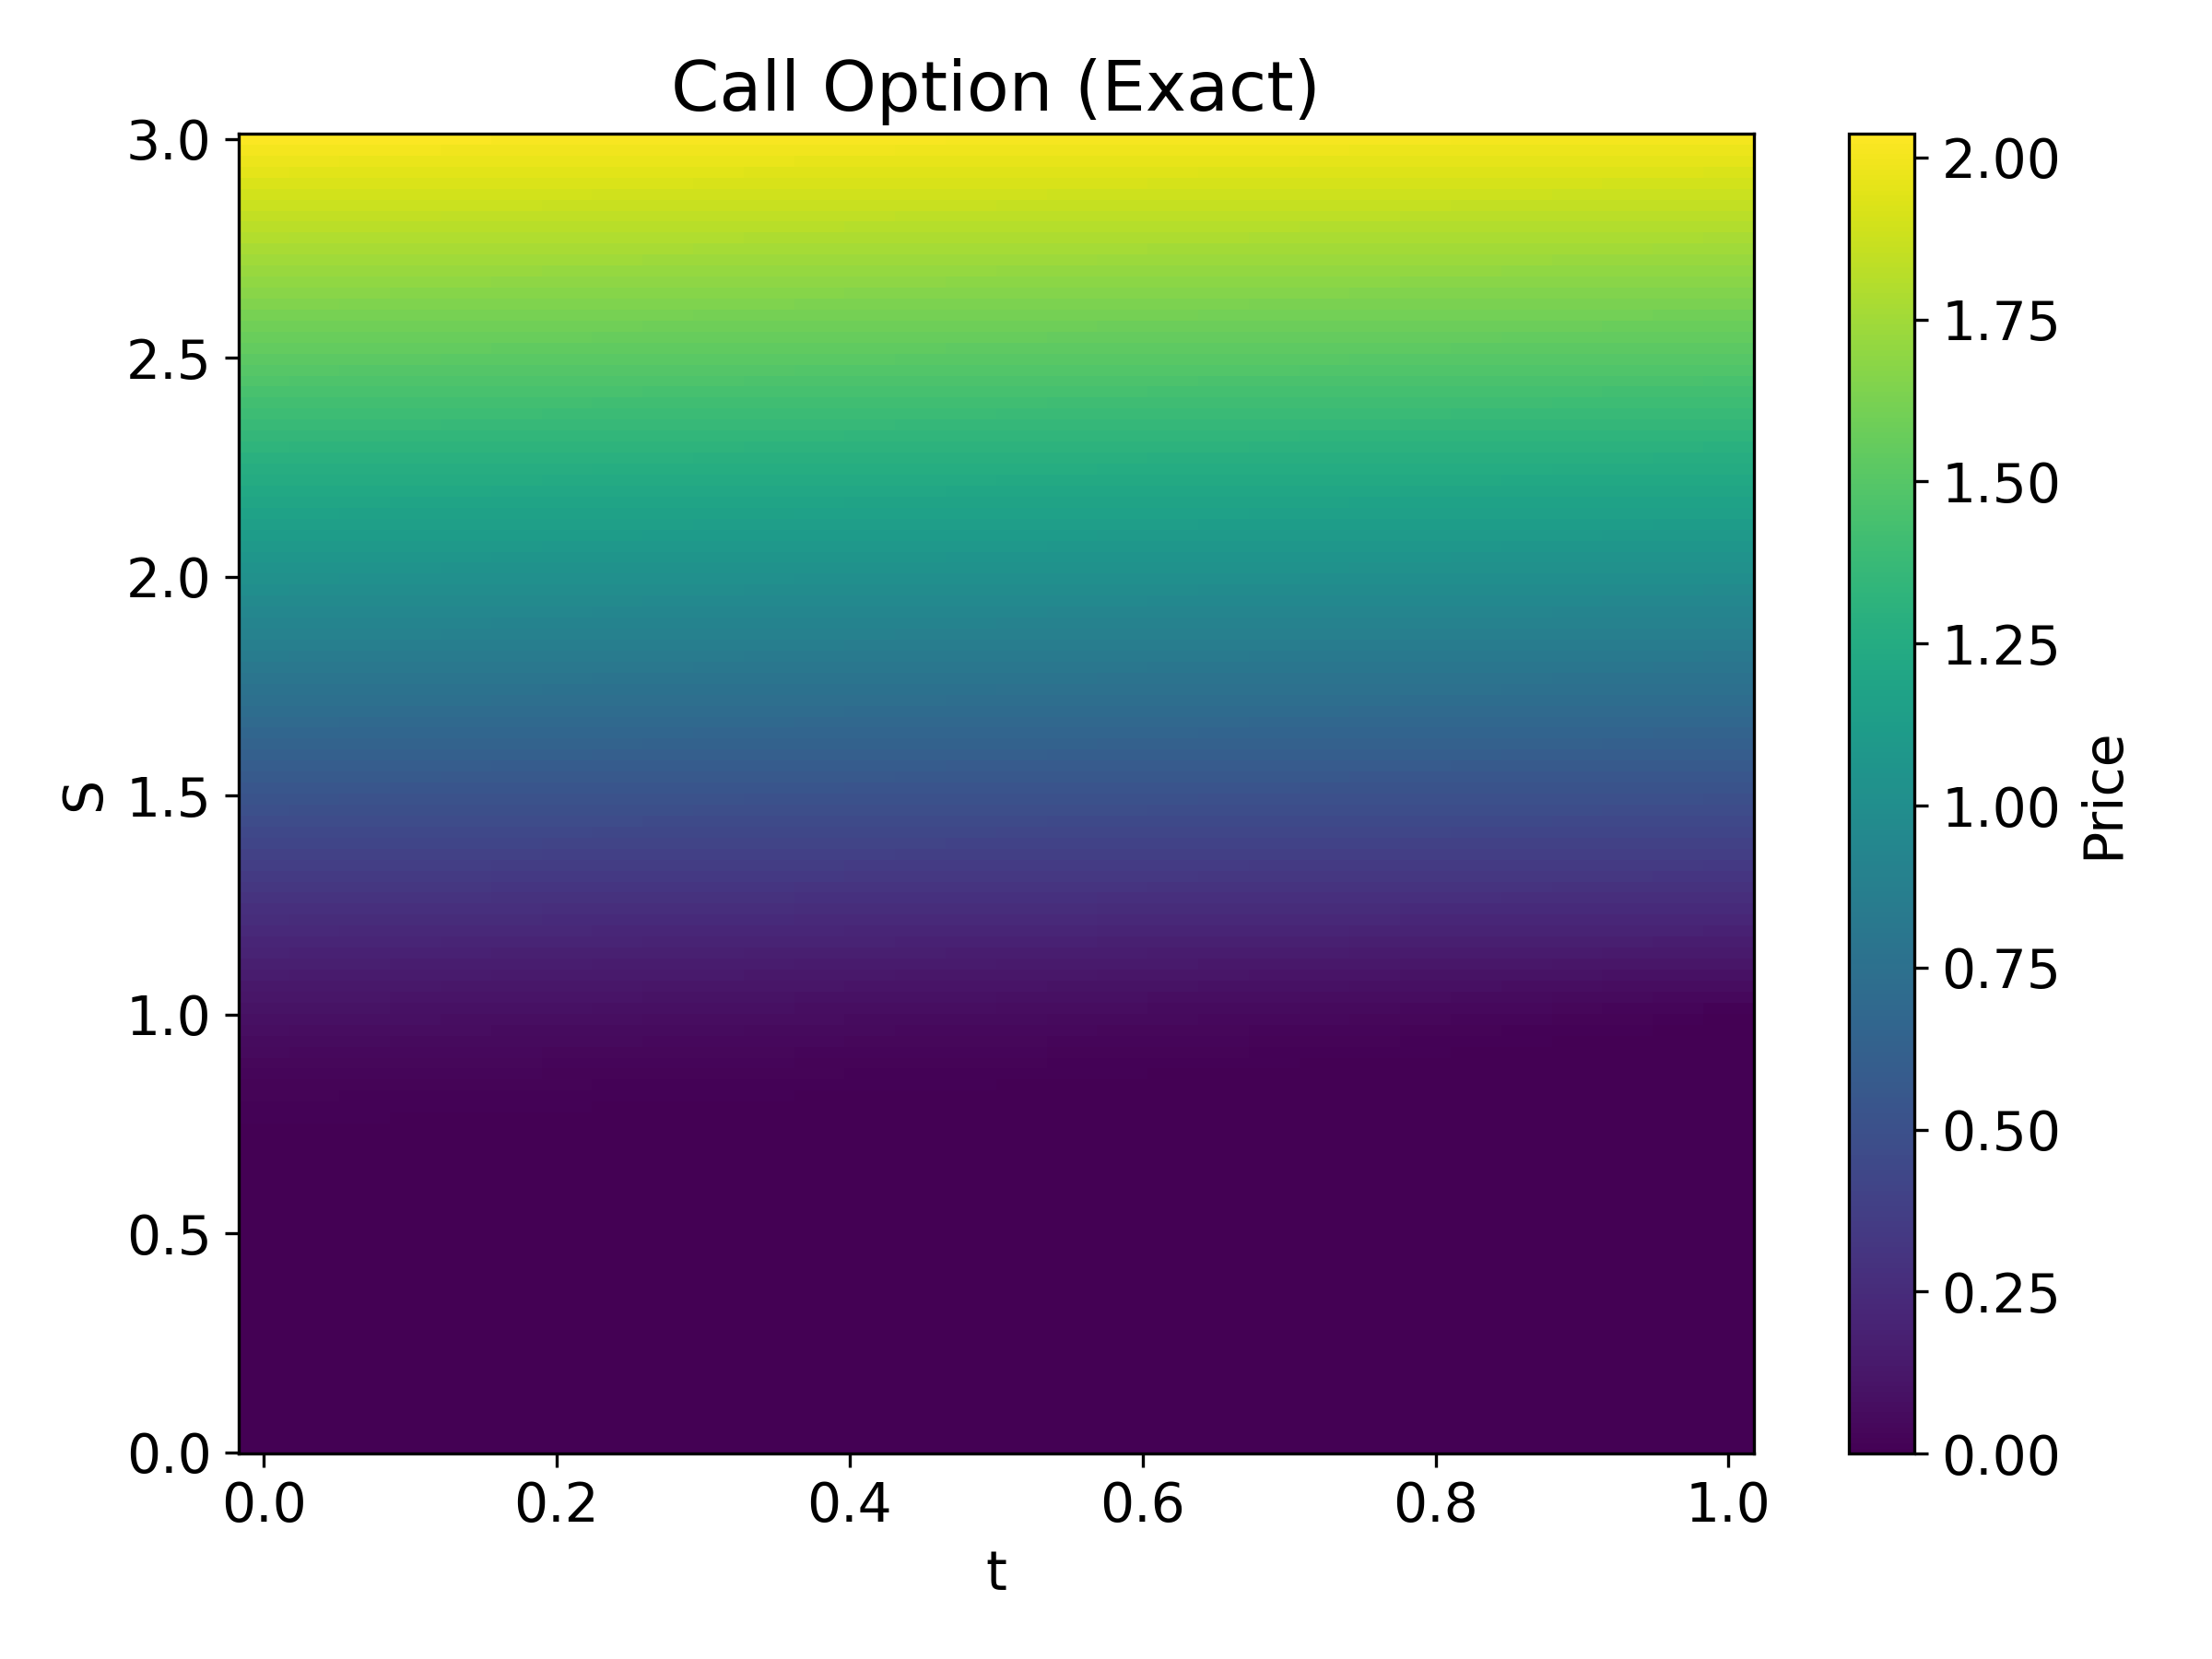
\includegraphics[width=\textwidth]{figures/call option Exact solution.jpg}
	\end{subfigure}
	\caption{欧式看涨期权Black-Schole方程SDE Monte Carlo求解（左）与PDE精确解（右）}
	\label{fig:4.1}
\end{figure}
\begin{figure}[htbp]
	\centering
	\begin{subfigure}[b]{0.45\textwidth}
		\centering
		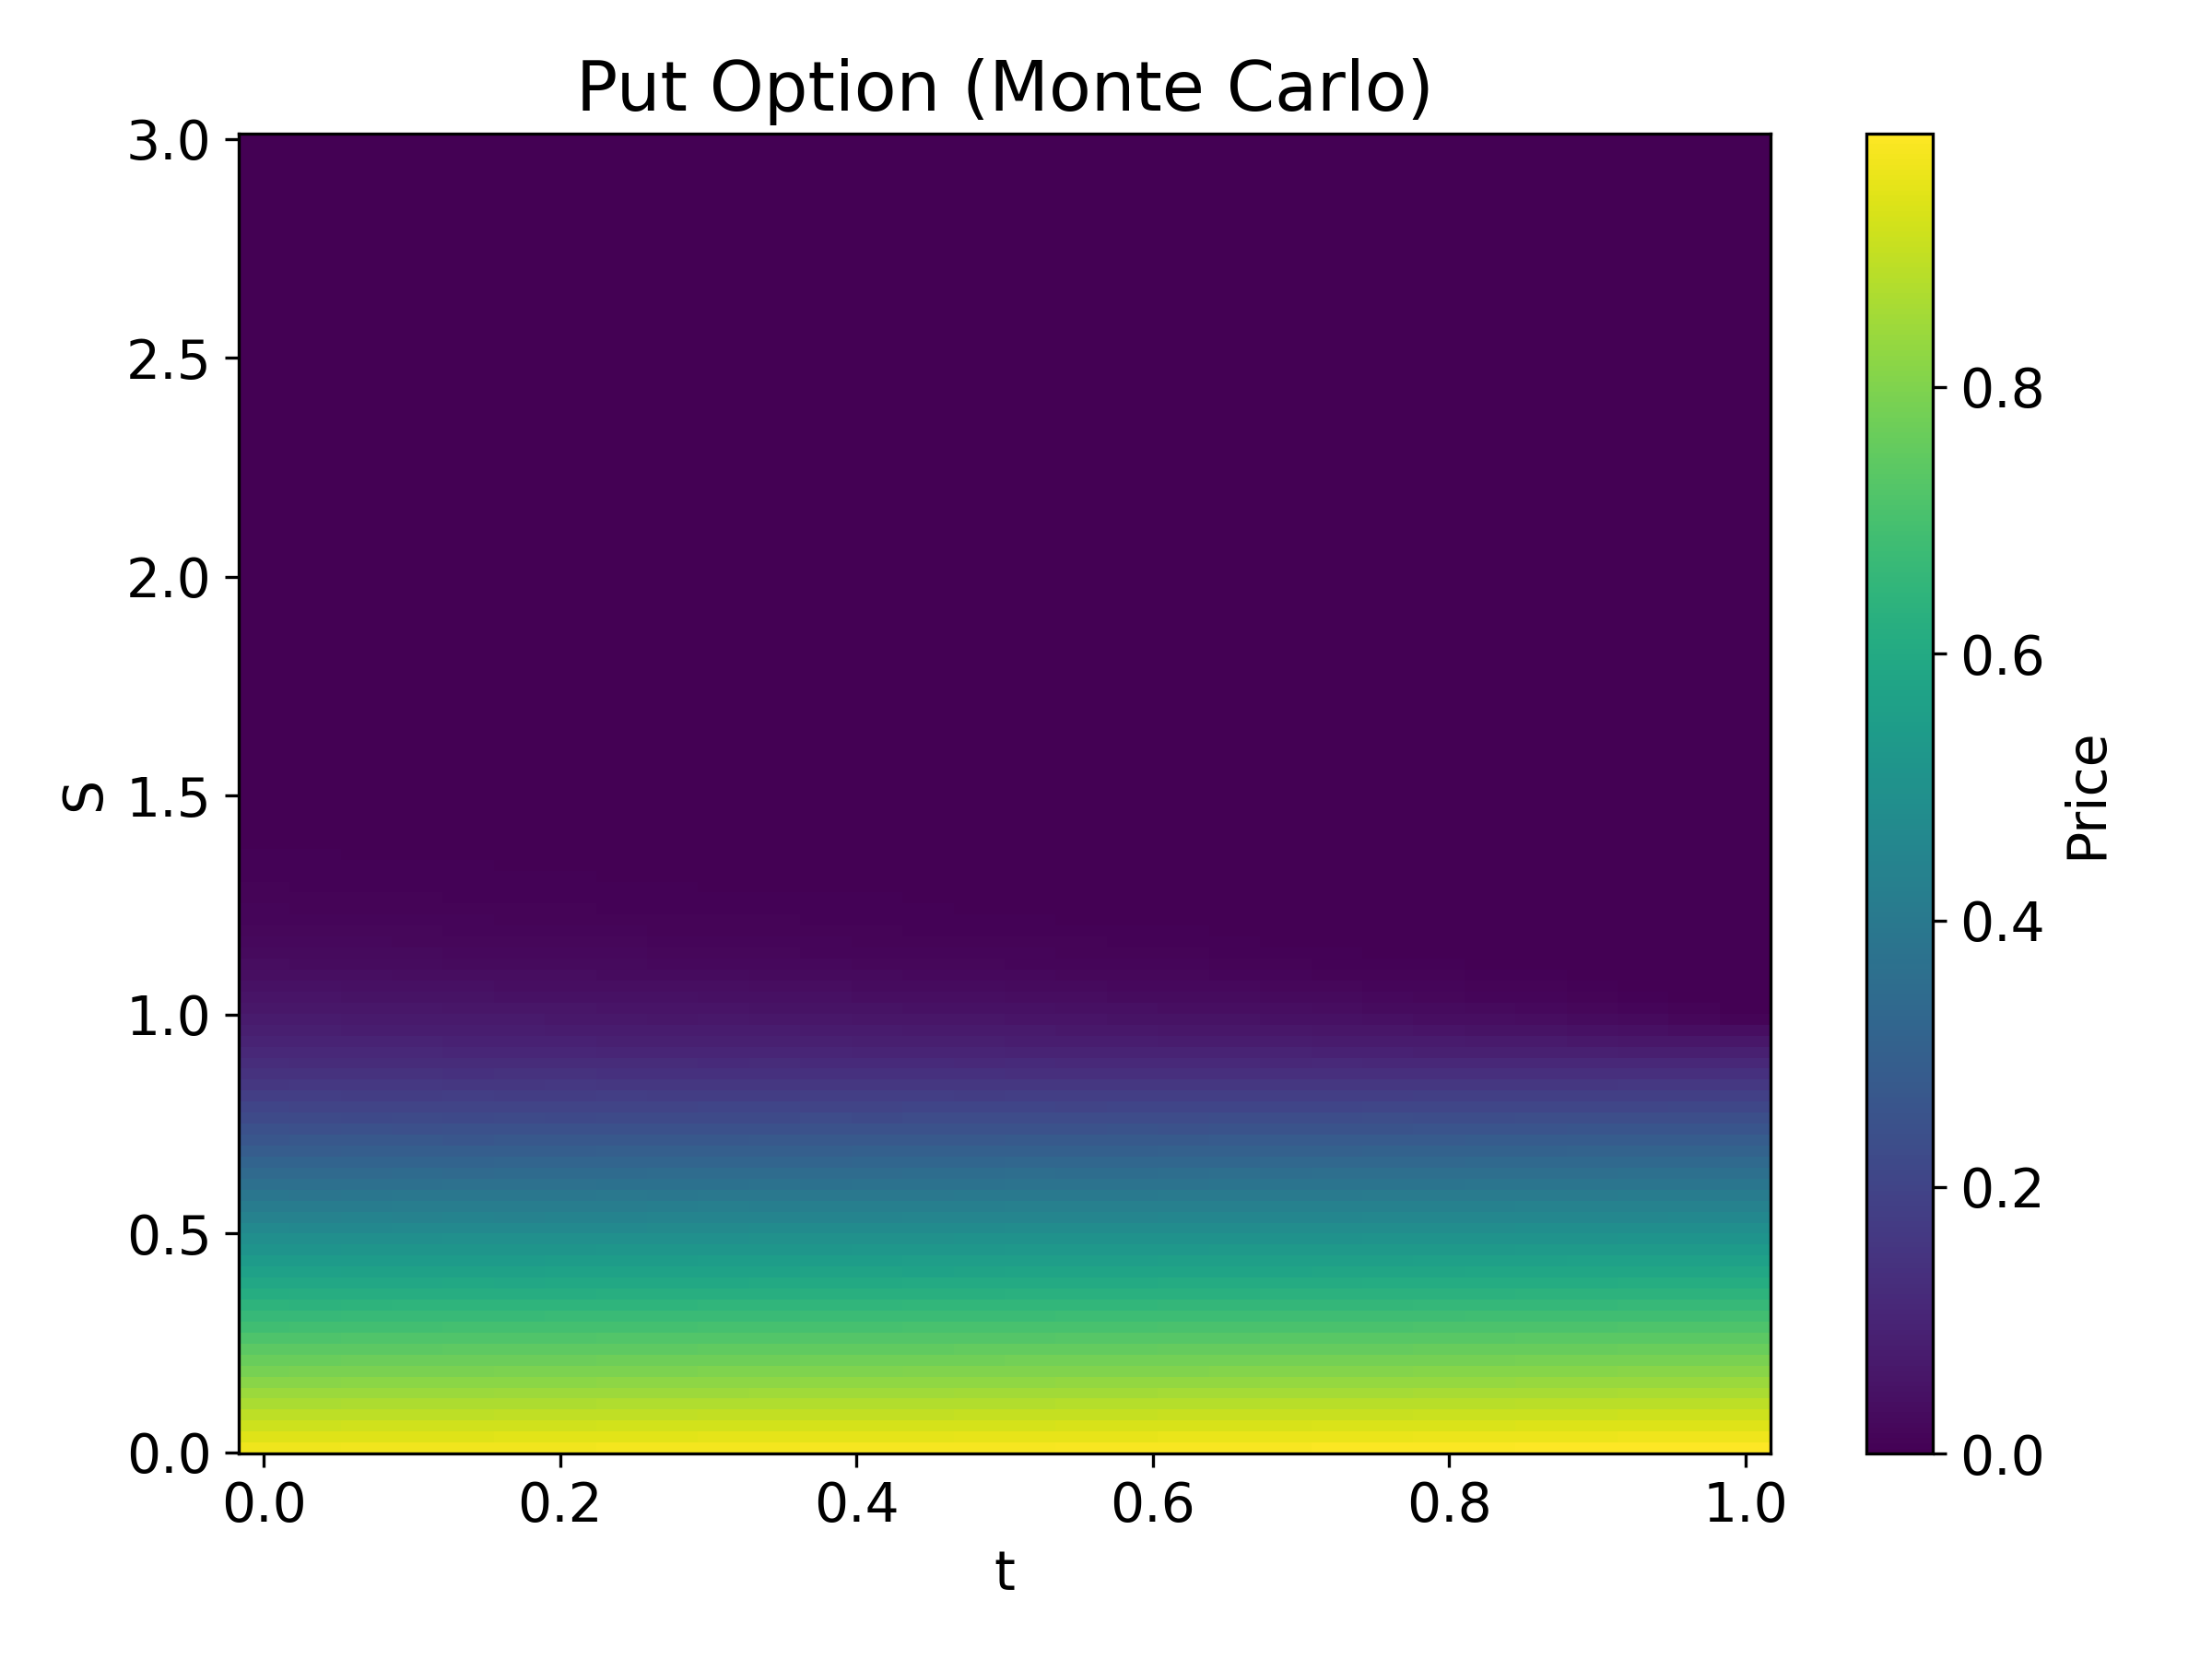
\includegraphics[width=\textwidth]{figures/put option MC solution.jpg}
	\end{subfigure}
	\hfill
	\begin{subfigure}[b]{0.45\textwidth}
		\centering
		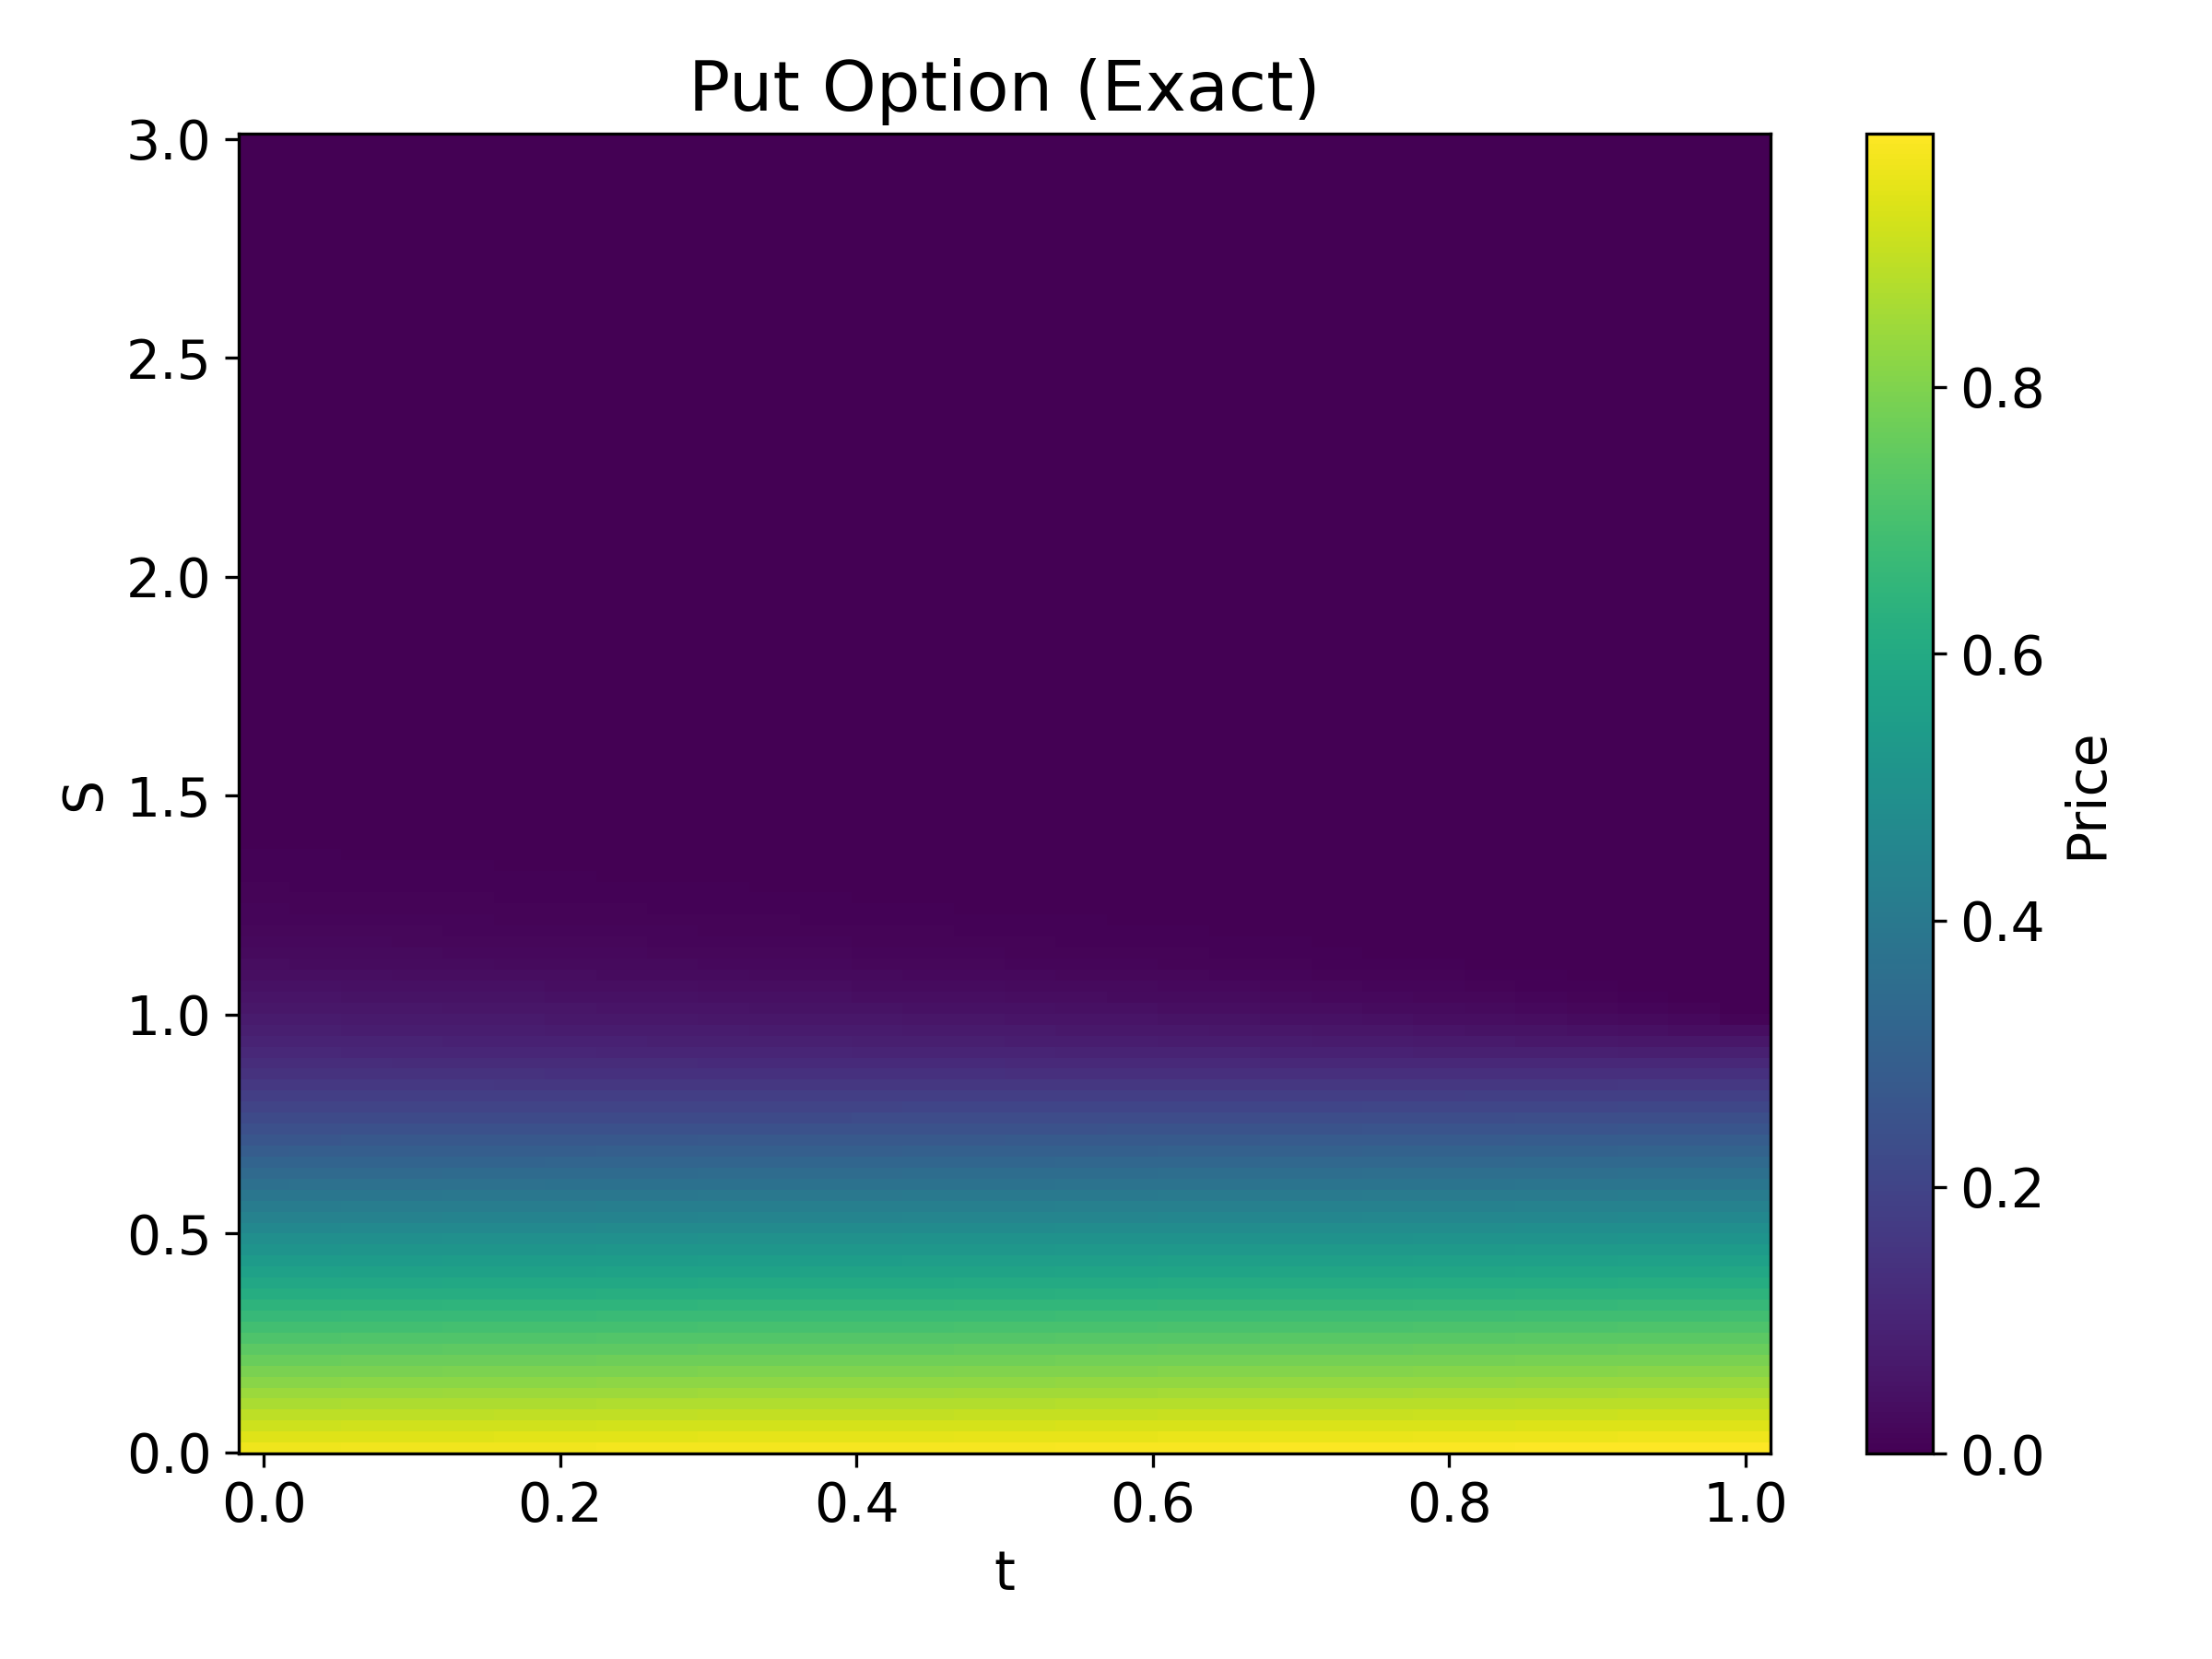
\includegraphics[width=\textwidth]{figures/put option Exact solution.jpg}
	\end{subfigure}
	\caption{欧式看跌期权Black-Schole方程SDE Monte Carlo求解（左）与PDE精确解（右）}
	\label{fig:4.2}
\end{figure}

\begin{figure}[htbp]
	\centering
	\begin{subfigure}[b]{0.45\textwidth}
		\centering
		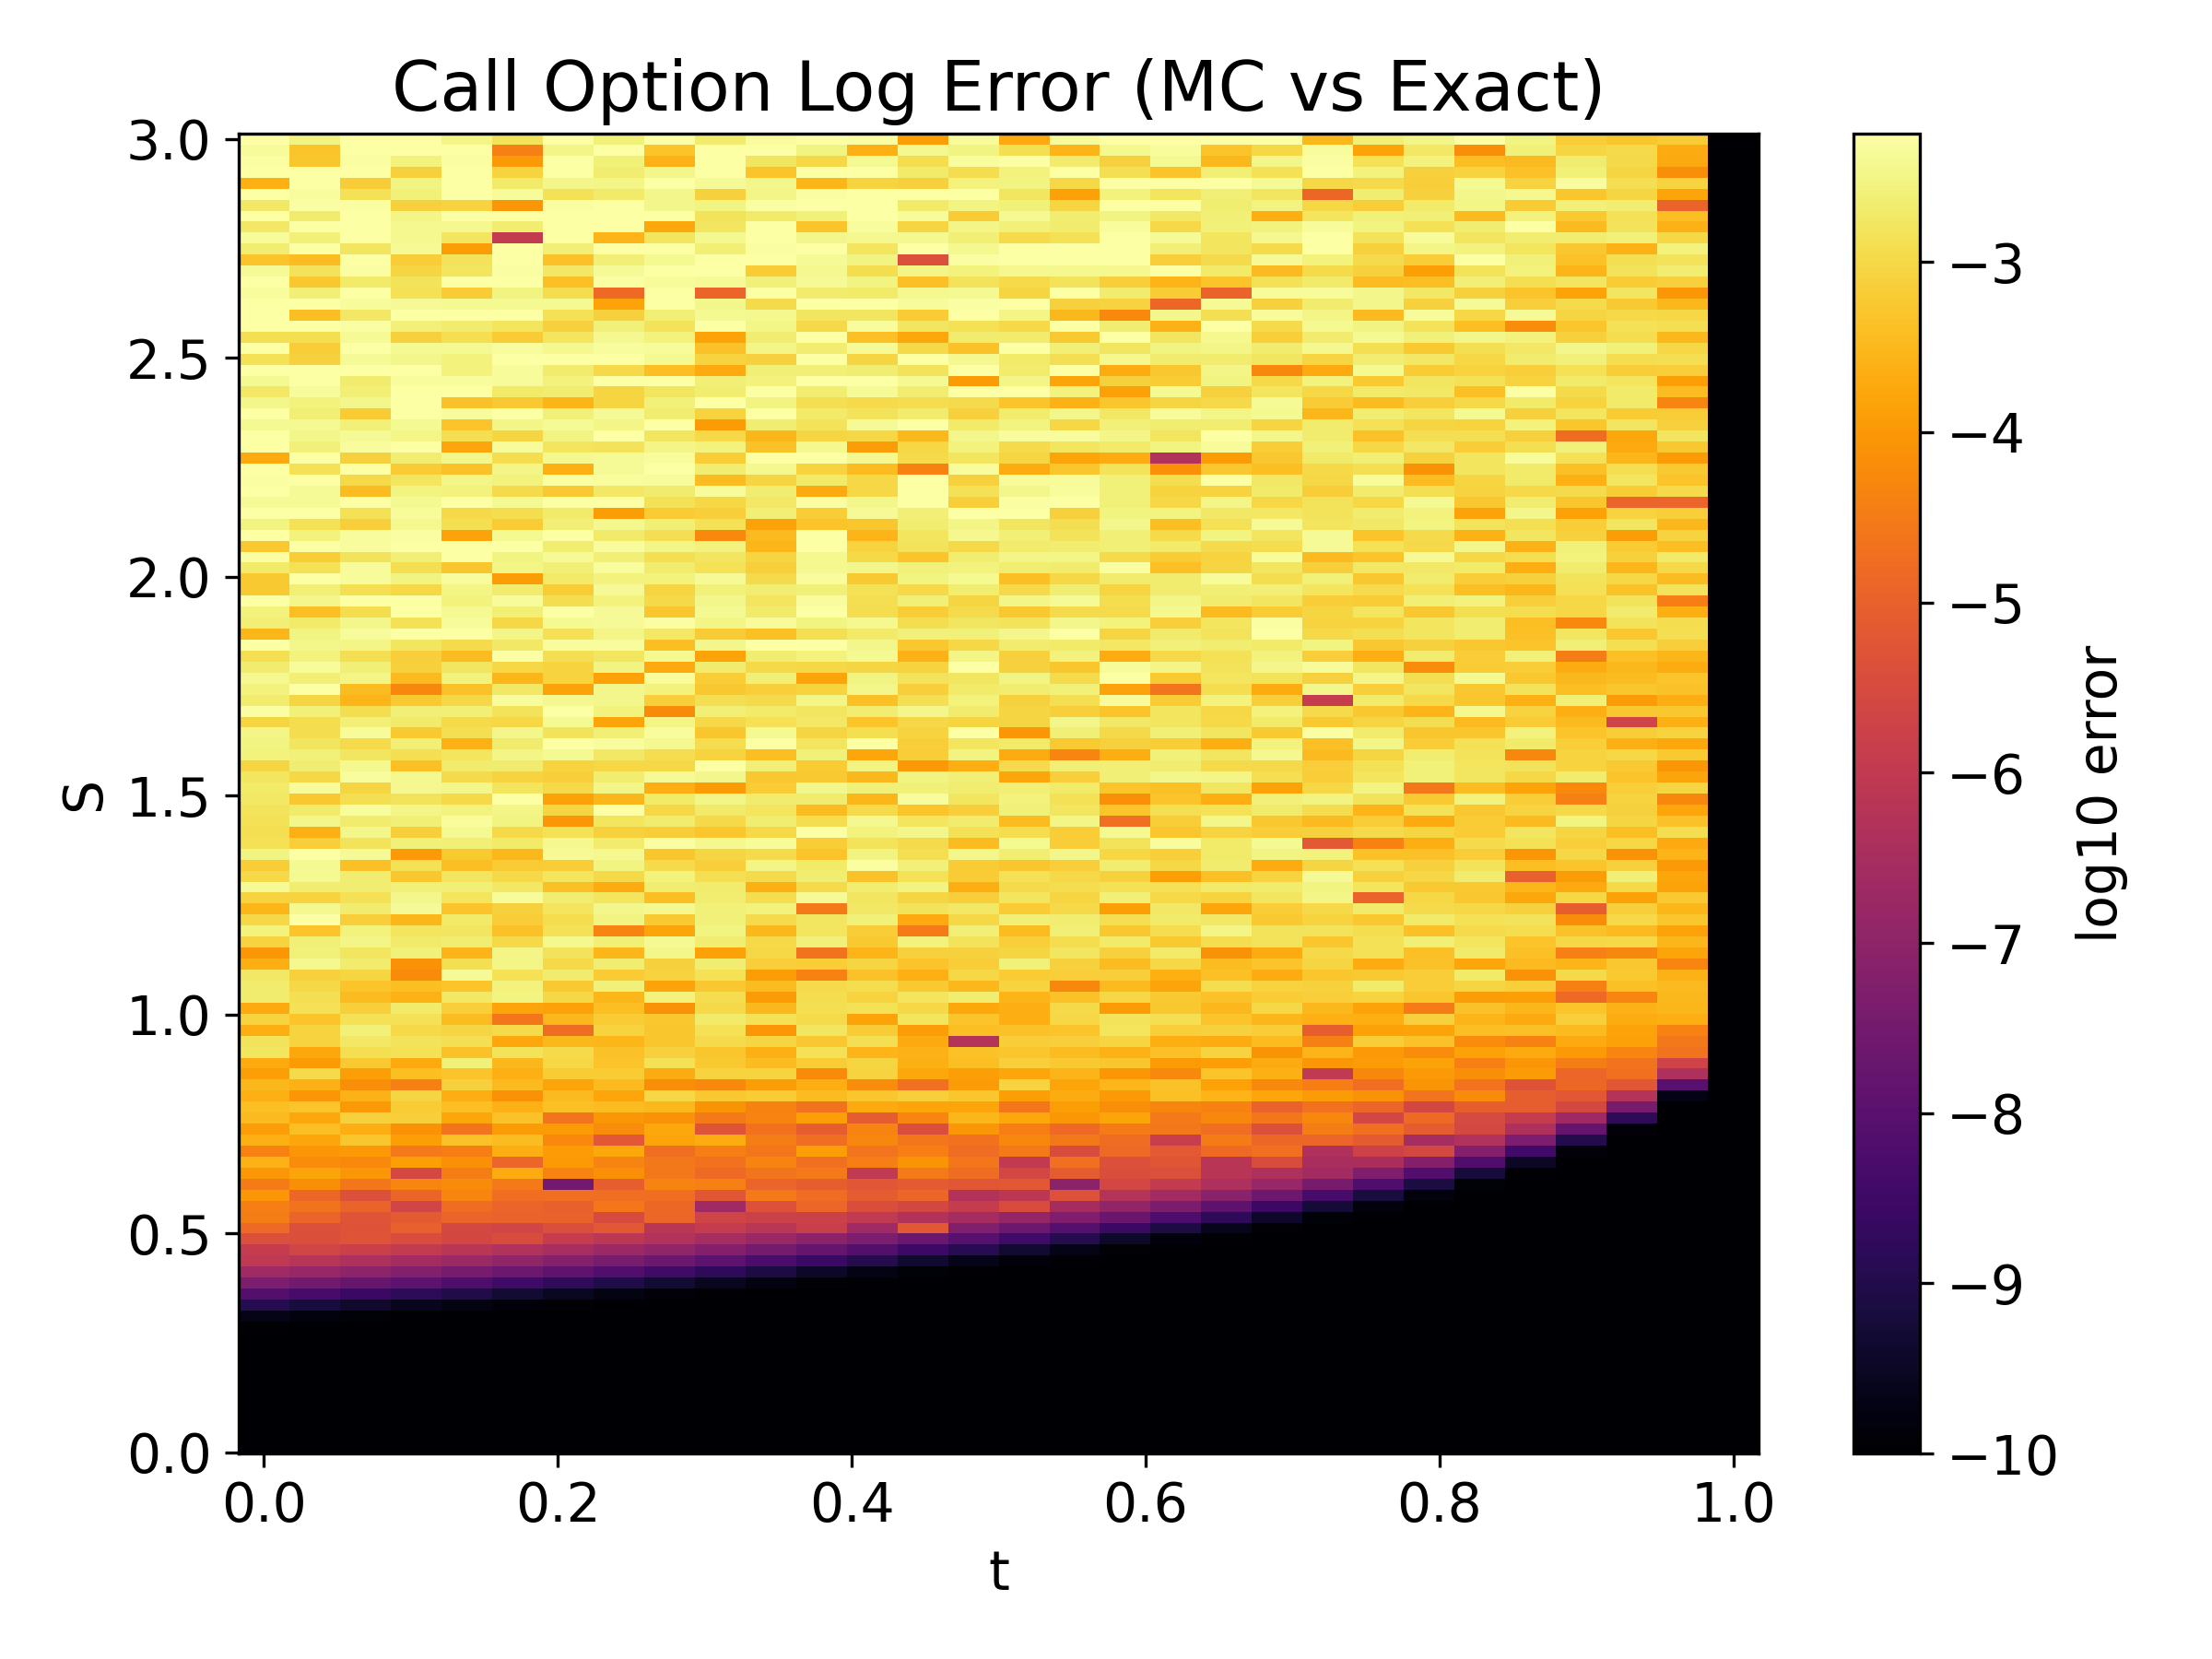
\includegraphics[width=\textwidth]{figures/call option error.png}
	\end{subfigure}
	\hfill
	\begin{subfigure}[b]{0.45\textwidth}
		\centering
		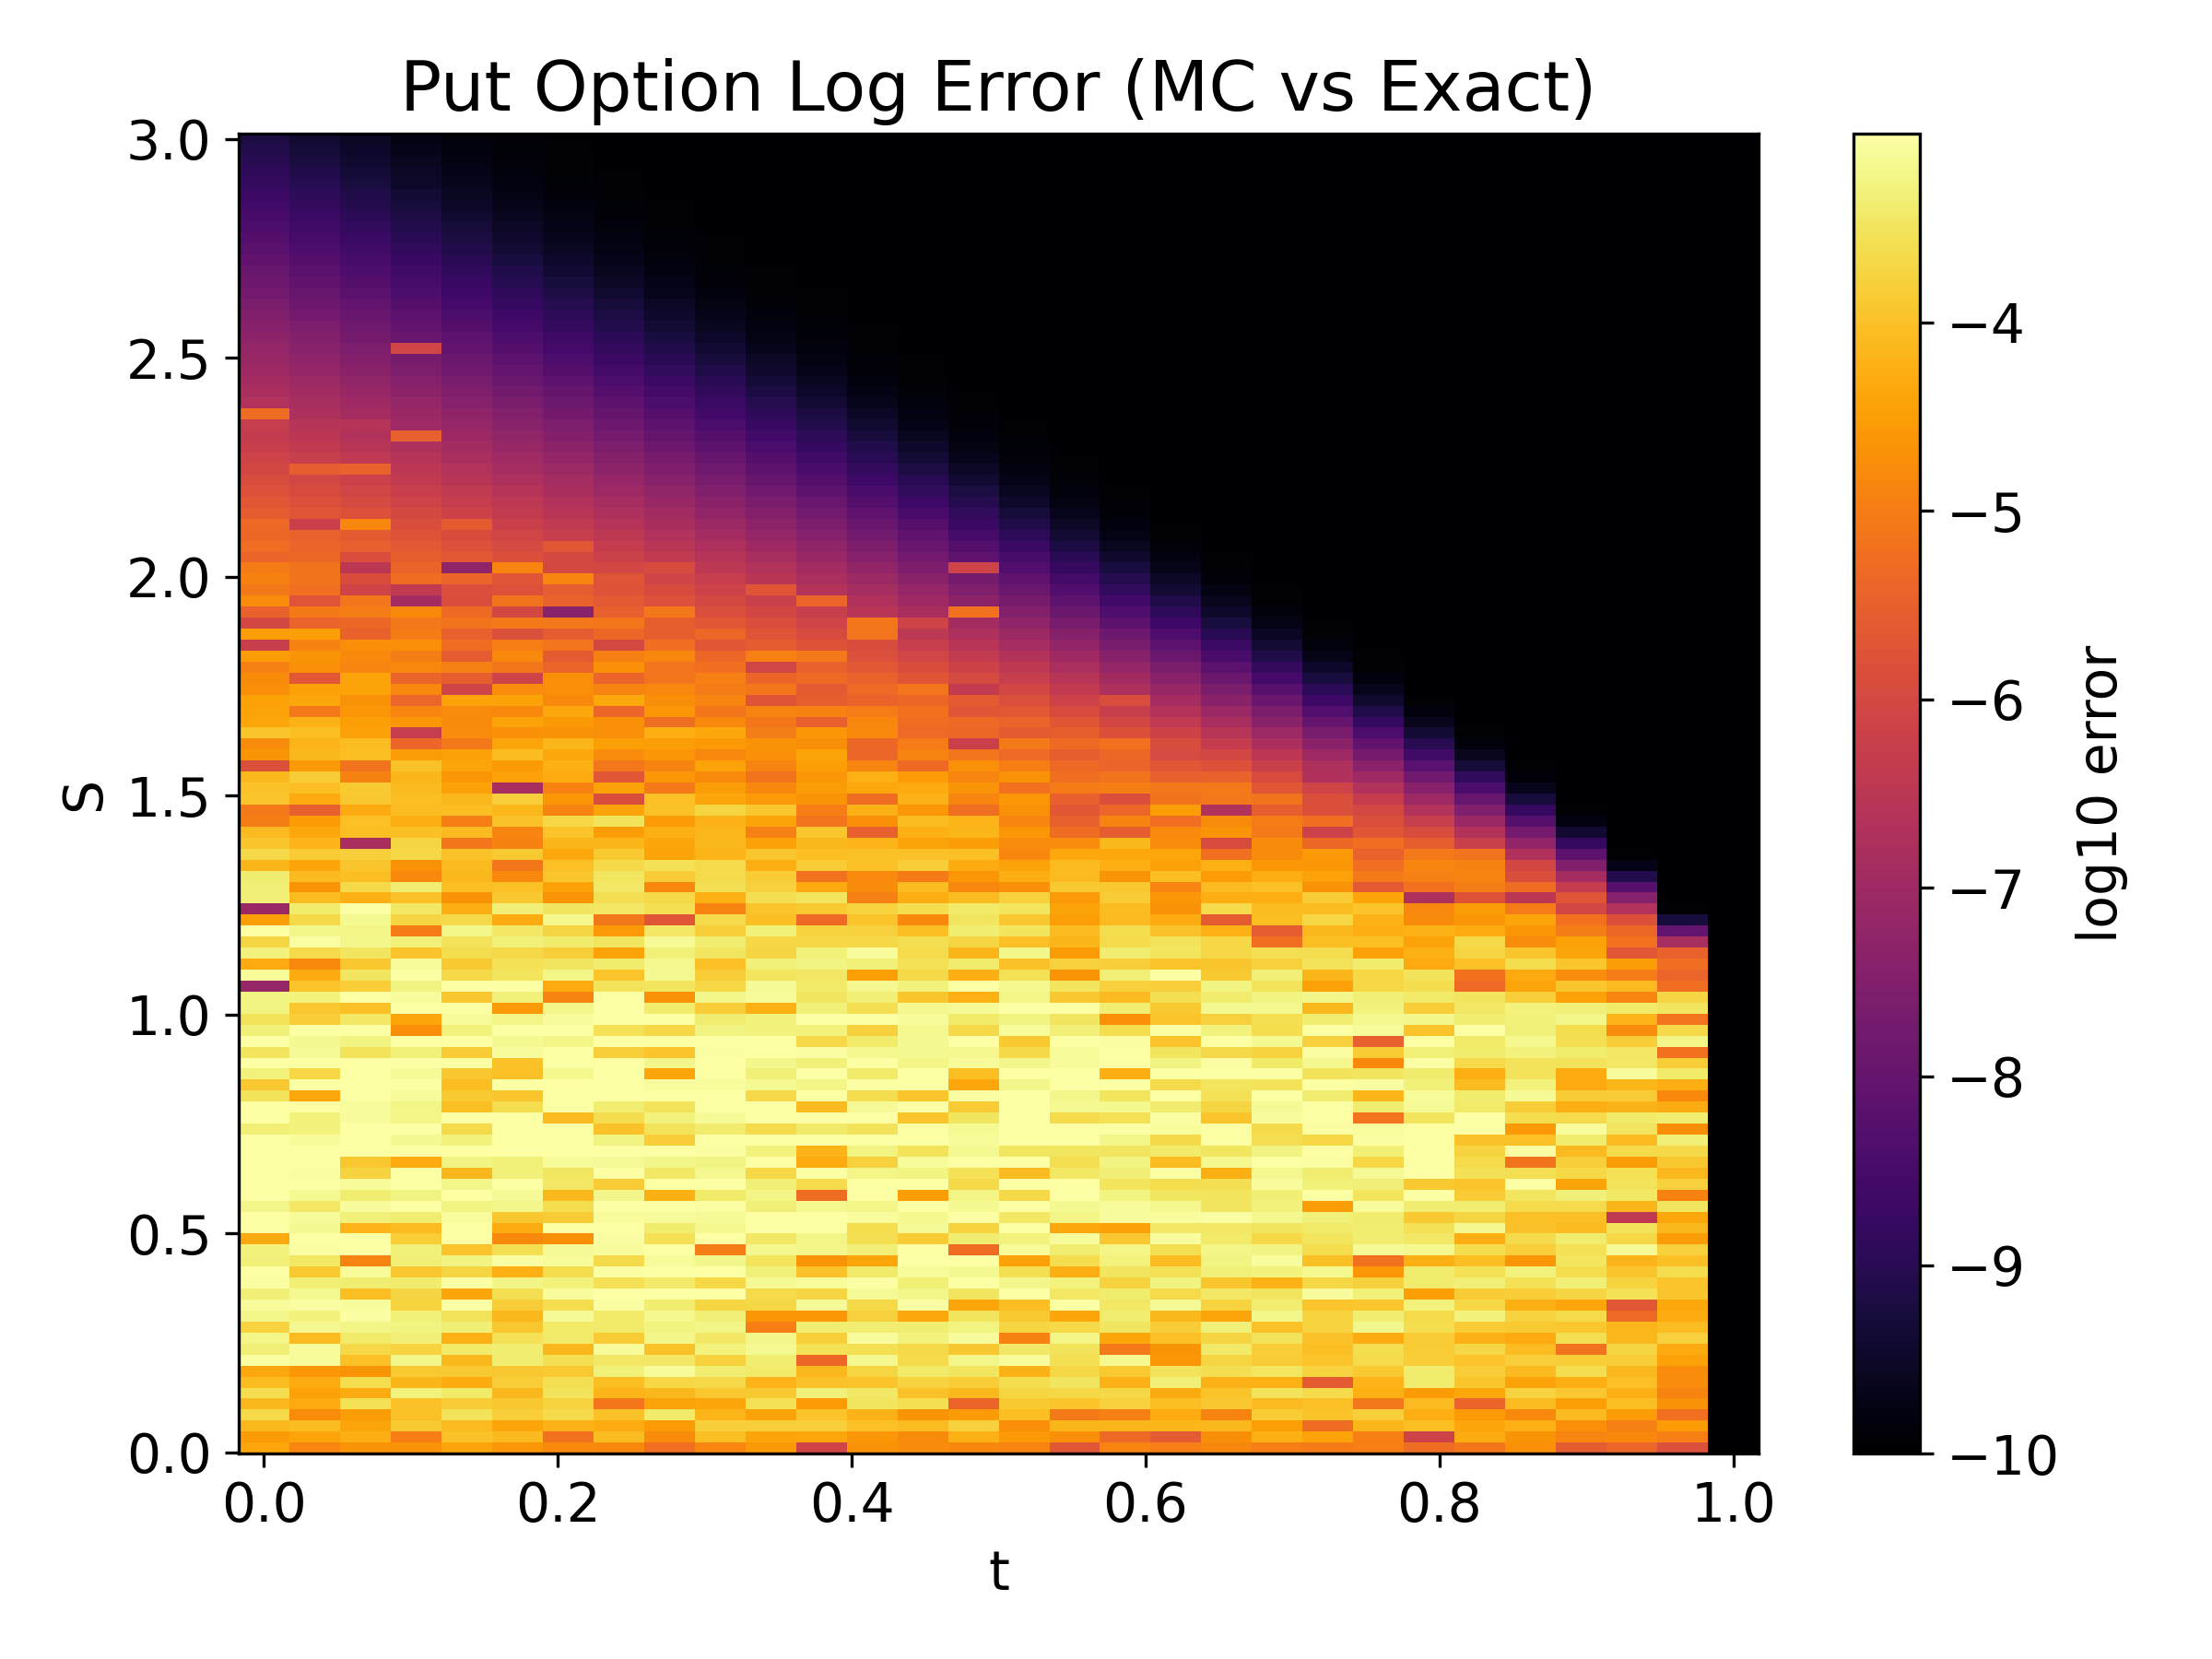
\includegraphics[width=\textwidth]{figures/put option error.png}
	\end{subfigure}
	\caption{欧式看涨期权（左）与欧式看跌期权（右）Black-Schole方程SDE Monte Carlo解与PDE精确解的对数误差}
	\label{fig:4.3}
\end{figure}

图\ref{fig:4.4}展示两个不同初值条件下SDE Monte Carlo解的实际收敛速率与理论收敛速率的对比。从两张子图不难看出，无论是欧式看涨期权还是欧式看跌期权条件下，SDE Monte Carlo方法应用在Black-Scholes方程求解上的误差收敛速率基本符合前文中对收敛速率的分析。因此如想继续降低误差可以通过增大Monte Carlo的路径数$M$来实现，且大致是路径数增加两个量级，误差减小一个量级。当然由于还受到离散化误差的影响，还需同时增大离散化区间数$N$。

\begin{figure}[htbp]
	\centering
	\begin{subfigure}[b]{0.45\textwidth}
		\centering
		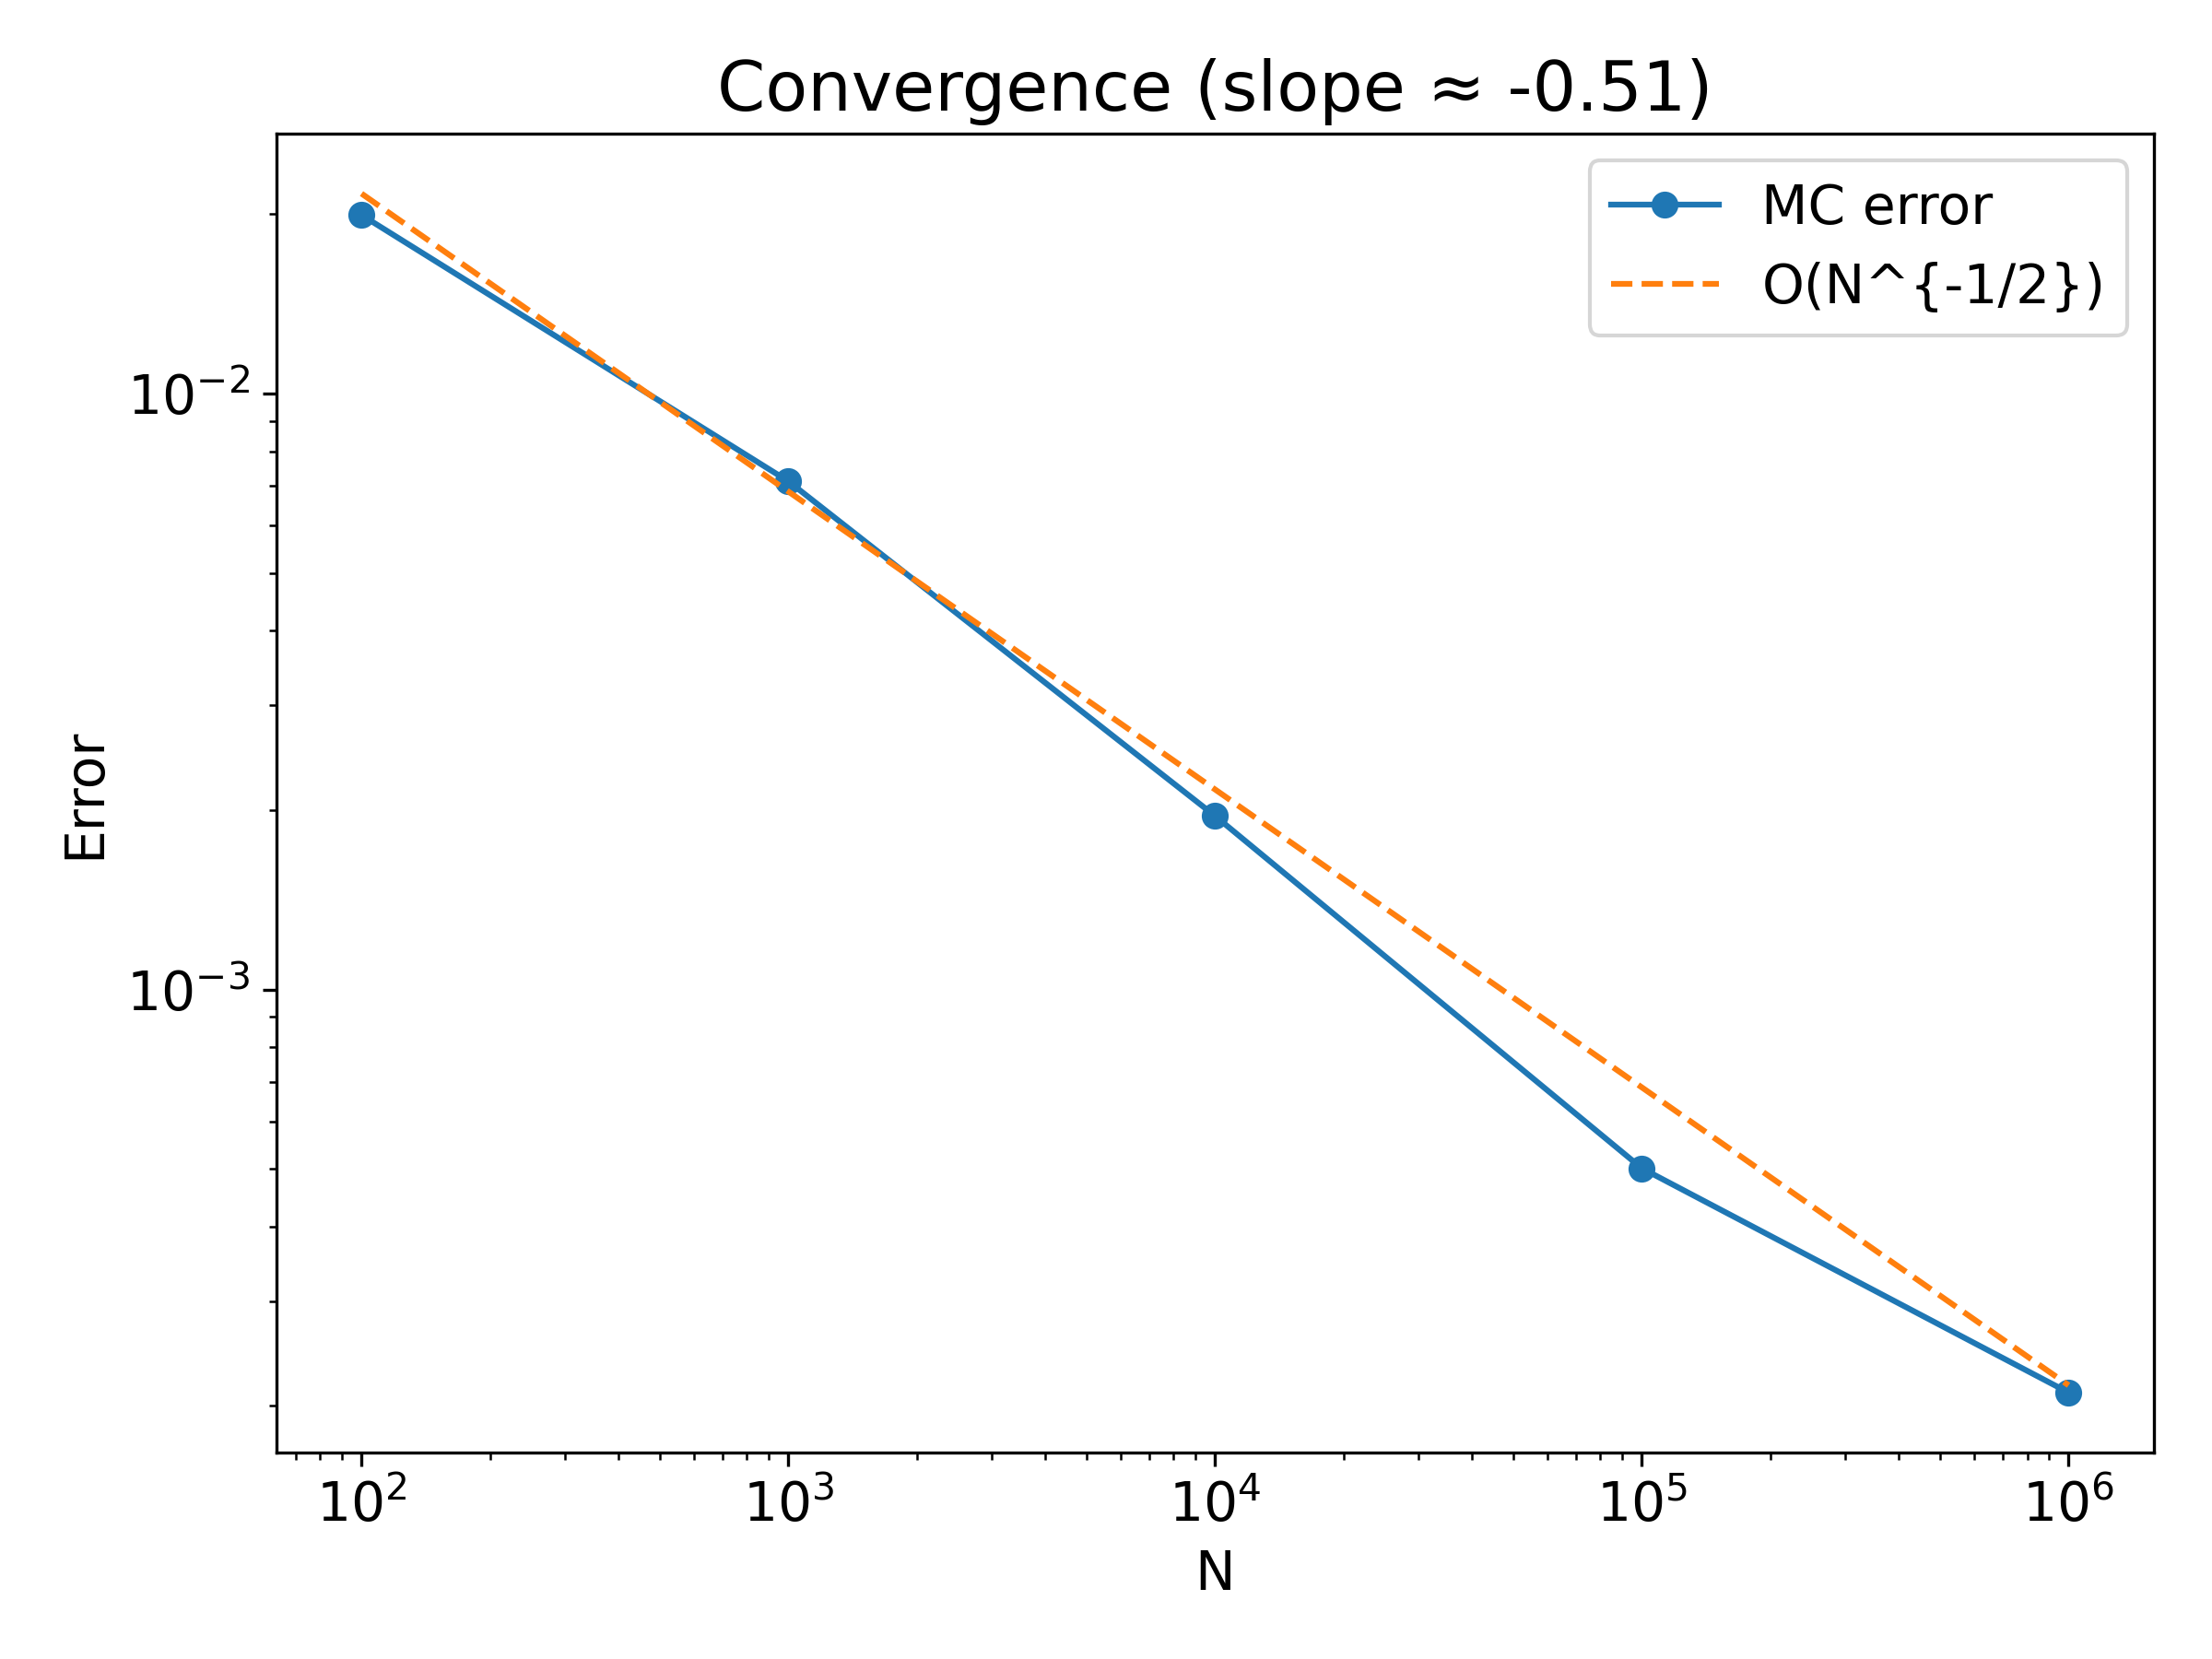
\includegraphics[width=\textwidth]{figures/call option convergence rate.jpg}
	\end{subfigure}
	\hfill
	\begin{subfigure}[b]{0.45\textwidth}
		\centering
		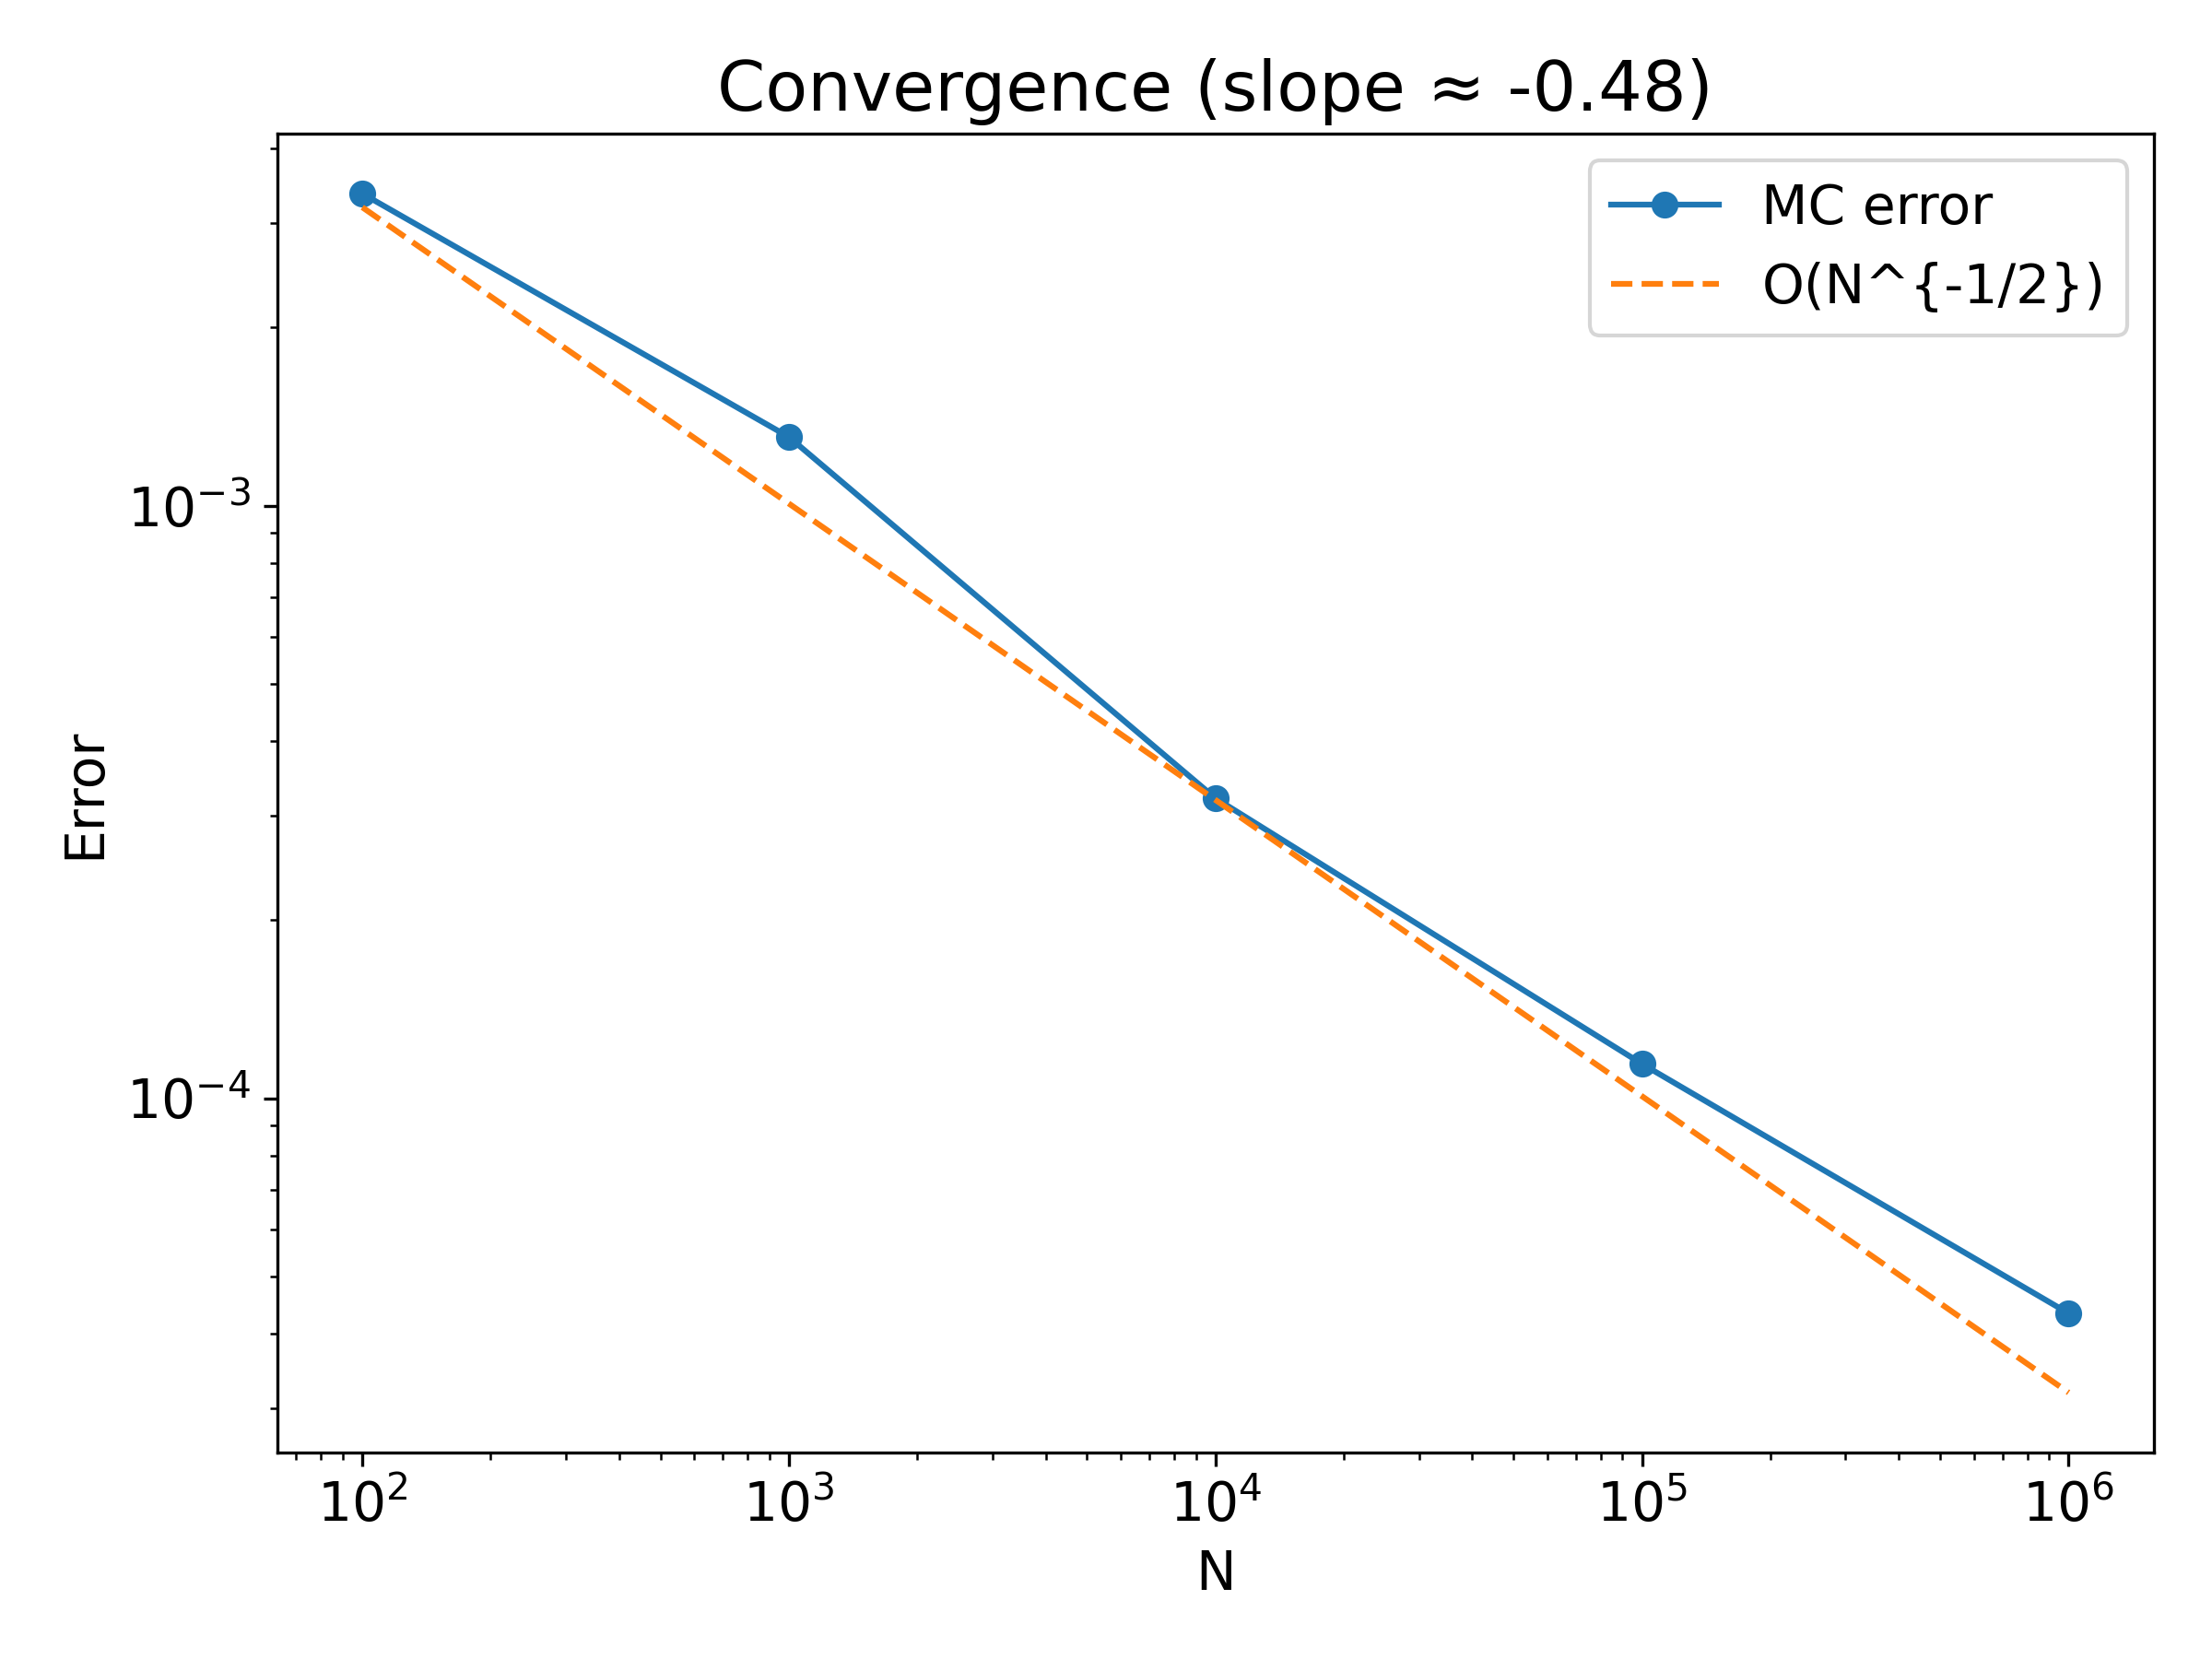
\includegraphics[width=\textwidth]{figures/put option convergence rate.jpg}
	\end{subfigure}
	\caption{欧式看涨期权（左）与欧式看跌期权（右）Black-Schole方程SDE Monte Carlo解实际收敛速率与理论收敛速率对比}
	\label{fig:4.4}
\end{figure}

综上，通过对以上结果分析足以说明，SDE Monte Carlo方法在求解Black-Scholes方程上的可行性。

\chapter{总结与展望}

本文以随机微分方程（SDE）及其在偏微分方程（PDE）求解中的应用为研究核心，系统地完成了从理论推演、算法构建到数值实验的完整研究闭环。在理论研究层面，本文通过对Brownian运动性质、It\^o积分构造及It\^o公式的应用研究，成功构建了随机分析的严谨数学基石，深入揭示了随机微分方程作为刻画带噪系统工具的独特优势，并阐明了其对应的无穷小生成元与二阶偏微分算子之间深刻的对偶关系，从而为 PDE 的概率化求解提供了坚实的理论支撑。通过详细论证，本文证明了 Feynman-Kac 公式及 Dirichlet-Poisson 问题解的存在唯一性，并说明其均可转化为扩散过程在随机停时或特定路径下的期望值，这一发现将复杂的算子求解问题有效地简化为随机轨迹的统计平均问题。

在数值实现与应用层面，本文设计并实现了基于 Euler-Maruyama 离散化方案的 Monte Carlo 概率算法。数值实验结果表明，该算法在处理如单位圆、正方形等不同几何区域的Dirichlet问题时展现出极高的灵活性，对于像三角形区域上的Dirichlet这种通常无显式PDE解的问题，可以考虑利用本文的数值方法进行求解。此外，本文将该理论框架成功应用于 Black-Scholes 期权定价模型，实验结果与解析解的高度吻合进一步验证了概率方法在处理金融波动等跨学科实际问题中的准确性与鲁棒性。综上所述，本文的研究工作不仅深化了对 SDE 与 PDE 对等性的理论认识，也为复杂方程的数值求解提供了一种稳定、高效且易于并行化的计算途径。

尽管本文在随机微分方程求解偏微分方程的理论与算法上取得了一定的进展，但仍存在诸多值得进一步深入探讨的方向。首先，在计算效率的进一步优化方面，目前采用的基础 Monte Carlo 模拟在样本量较小时仍存在统计波动，未来研究可尝试引入重要性采样、控制变量法或拟Monte Carlo方法等高级方差缩减技术，以在保证精度的前提下显著提升收敛速度。其次，本文目前的研究范畴主要集中在线性 PDE 的概率解，对于非线性或高阶偏微分方程（如半线性热方程或复杂的流体力学方程），其对应的随机模型通常涉及更为复杂的倒向随机微分方程或分支扩散过程，探索这些复杂方程的概率数值解法将是未来研究的重要突破口。

此外，随着人工智能技术的飞速发展，将机器学习与随机模拟相结合已成为科学计算的前沿趋势。探索如何利用深度学习的函数逼近能力来辅助 SDE 的路径采样，或是利用深度学习求解SDE，如，将物理信息神经网络（PINN）运用到求解的SDE上等，有望为解决极高维度的物理与金融建模问题提供全新的视角。最后，考虑到随机路径模拟具有天然的并行特性，未来可以进一步探索在 GPU 或分布式计算平台上的算法实现，通过优化并行计算架构，实现对大规模复杂动力系统的高效实时数值模拟。总之，随机微分方程为理解和解决确定性问题提供了一个全新的随机维度，随着计算数学理论与技术的不断进步，这一领域的研究必将在工程实践与科学探索中发挥愈发关键的作用。


\appendix

\chapter{}\label{A}

附录\label{A}中定理均来自于B.\O ksendal的随机微分方程教材\cite{SDE_book_BO}。

\begin{theorem}[Kolmogorov扩张定理]\label{theo:Kol_expan}
	$\forall t_1\ldots t_k\in T,k\in \textbf{N}$，对任意$\mathbb{R}^n$上Borel集$F_i$，令$\nu_{t_1,\ldots,t_k}$为$\mathbb{R}^{nk}$上概率测度，使得
	\[
	\nu_{t_{\sigma(1)}, \cdots, t_{\sigma(k)}}(F_1 \times \cdots \times F_k) = \nu_{t_1, \cdots, t_k}(F_{\sigma^{-1}(1)} \times \cdots \times F_{\sigma^{-1}(k)}).
	\]
	对$\left\{1,2\ldots,k\right\}$的任一排列$\sigma$均成立，以及满足
	\[
	\nu_{t_1, \dots, t_k} (F_1 \times \cdots \times F_k) = \nu_{t_1, \dots, t_k, t_{k+1}, \dots, t_{k+m}} (F_1 \times \cdots \times F_k \times \mathbf{R}^n \times \cdots \times \mathbf{R}^n).
	\]
	则存在一概率空间$(\Omega,\mathcal{F},P)$以及一$\Omega$上随机过程$\left \{ X_t(\omega)\right \}_{t\in T},X_t:\to \mathbb{R}^n$使
	\[
	\nu_{t_1, \dots, t_k} (F_1 \times \cdots \times F_k) = P(X_{t_1}\in F_1,\ldots,X_{t_k}\in F_k).
	\]
	$\forall t_i\in T,k\in \textbf{N}$及任意$\mathbb{R}^n$上Borel集$F_i$均成立。
\end{theorem}

\begin{theorem}[Kolmogorov连续性定理]\label{theo:Kol_continuity}
	若随机过程$\left \{ X_t\right \}_{t\ge 0}$满足：$\forall T>0$，存在正常数$\alpha,\beta,D$使得
	\[
	\mathbb{E}\left\vert X_t-X_s\right\vert^\alpha\le D\left\vert t-s\right\vert^{1+\beta},\hspace{0.3cm} 0\le s,t\le T.
	\]
	则$\left \{ X_t\right \}_{t\ge 0}$存在一连续版本。
\end{theorem}

\begin{theorem}[基本函数的It\^o等距]\label{theo:Ito_isometry_fund}
	若$\phi(t,\omega)$为一有界基本函数，则有
	\[
	\mathbb{E}\left[ (\int_{S}^{T}\phi(t,\omega)dB_t)^2\right]=\mathbb{E}\left[ \int_{S}^{T}\phi^2(t,\omega)dt\right].
	\]
\end{theorem}

由此从基本函数出发，通过以下几个引理来定义$\mathcal{V}$中一般函数的It\^o积分。

\begin{theorem}[从基本函数到有界样本路径连续函数]\label{theo:step1_to_build}
	令$g\in\mathcal{V}$有界，且$g(\cdot,\omega)$对每一个$\omega$都是连续的，则存在一$\mathcal{V}$中基本函数列$\left\{\phi_n\right\}$使得
	\[
	\mathbb{E}\left[\int_{S}^{T}(g-\phi_n)^2dt\right]\to 0,\hspace{0.3cm}n\to\infty.
	\]
\end{theorem}

\begin{theorem}[从有界样本路径连续函数到有界函数]\label{theo:step2_to_build}
	令$h\in\mathcal{V}$有界的，则存在一有界样本路径连续函数列$\left\{g_n\right\}\in\mathcal{V}$使得
	\[
	\mathbb{E}\left[\int_{S}^{T}(h-g_n)^2dt\right]\to 0,\hspace{0.3cm}n\to\infty.
	\]
\end{theorem}

\begin{theorem}[从有界函数到$\mathcal{V}$中的一般函数]\label{theo:step3_to_build}
	设$f\in\mathcal{V}$，则存在一$\mathcal{V}$中有界函数列$\left\{h_n\right\}$使
	\[
	\mathbb{E}\left[\int_{S}^{T}(f-h_n)^2dt\right]\to 0,\hspace{0.3cm}n\to\infty.
	\]
\end{theorem}

从定义出发有以下两个简单推论。

\begin{corollary}[一般函数的It\^o等距]\label{cor:Ito_isometry_general}
	\[
	\mathbb{E}\left[(\int_{S}^{T}f(t,\omega)dB_t)^2\right]=\mathbb{E}\left[\int_{S}^{T}f^2(t,\omega)dt\right],\hspace{0.3cm}\forall f\in\mathcal{V}(S,T).
	\]
\end{corollary}

\begin{corollary}\label{cor:Ito_int_convergency}
	若$f(t,\omega)\in\mathcal{V}(S,T)$且$f_n(t,\omega)\in\mathcal{V}(S,T)$，对$n=1,2,\ldots$且
	\[
	\mathbb{E}\left[\int_{S}^{T}(f_n-f)^2 dt\right]\to 0,\hspace{0.3cm}n\to\infty.
	\]
	故
	\[
	\int_{S}^{T}f_n(t,\omega)dB_t\xrightarrow{L^2(P)}\int_{S}^{T}f(t,\omega)dB_t,\hspace{0.3cm}n\to\infty.
	\]
\end{corollary}

\begin{theorem}[It\^o积分的简单性质]\label{theo:Ito_int_property}
	令$f,g\in\mathcal{V}(0,T)$且$0\le S<U<T$，则有
	\begin{enumerate}[label=(\arabic*)]
		\item $\int_{S}^{T}fdB_t=\int_{S}^{U}fdB_t+\int_{U}^{T}fdB_t,a.a.\omega$;
		\item $\int_{S}^{T}(cf+g)dB_t=c\int_{S}^{T}fdB_t+\int_{S}^{T}gdB_t,a.a.\omega$（c为常数）;
		\item $\mathbb{E}\left[\int_{S}^{T}fdB_t\right]=0$.
		\item $\int_{S}^{T}fdB_t$使$\mathcal{F}_T-$可测的.
	\end{enumerate}
\end{theorem}

\begin{theorem}[Doob's鞅不等式]\label{theo:Doob_martingale_inequaty}
	若$M_t$是（关于自身生成的$\sigma$代数流）一鞅，且$t\mapsto M_t(\omega)$是连续的$a.s.$，则$\forall p\ge 1,T\ge 0,\lambda>0$，有
	\[
	P[\sup_{0\le t\le T}\left\vert M_t\right\vert\ge\lambda]\le\frac{1}{\lambda^p}\mathbb{E}[\left\vert M_T\right\vert^p].
	\]
\end{theorem}

\begin{theorem}[It\^o积分连续版本定理]\label{theo:Ito_int_continuity}
	令$f\in\mathcal{V}(0,T)$，则It\^o积分
	\[
	\int_{0}^{t}fdB_s;0\le t\le T.
	\]
	存在一$(\Omega,\mathcal{F},P)$上的连续版本$J_t$使得
	\[
	P\left[J_t=\int_{0}^{t}fdB\right]=1.
	\]
\end{theorem}

\begin{theorem}[It\^o积分的鞅性]\label{theo:Ito_int_martingale}
	令$f(t,\omega)\in\mathcal{V}(0,T)$对任意$T$成立，则由It\^o积分定义的随机过程
	\[
	M_t(\omega)=\int_{0}^{t}f(s,\omega)dB_s.
	\]
	是关于$\left\{\mathcal{F}_t\right\}$的鞅，且有
	\[
	P[\sup_{0\le t\le T}\left\vert M_t\right\vert\ge\lambda]\le\frac{1}{\lambda^2}\cdot \mathbb{E}\left[\int_{0}^{T}f^2(s,\omega)ds\right];\hspace{0.3cm}\lambda,T>0.
	\]
\end{theorem}

\begin{theorem}[It\^o表示定理]\label{theo:Ito_represent}
	设$F\in L^2(\mathcal{F}_t^{(n)},P)$，则存在唯一的随机过程$f(t,\omega)\in\mathcal{V}^n(0,T)$使得
	\[
	F(\omega)=\mathbb{E}[F]+\int_{0}^{T}f(t,\omega)dB(t).
	\]
\end{theorem}

\begin{theorem}[鞅表示定理]\label{theo:martingale_represent}
	设$B(t)=(B_1(t),\ldots,B_n(t))$维$n$维Brownian运动，$M_t$为关于$\mathcal{F}_t^{(n)}$的鞅，$M_t\in L^2(P),\forall t\ge 0$。则存在唯一过程$g(s,\omega)\in\mathcal{V}^n(0,t),\forall t\ge 0$使得
	\[
	M_t(\omega)=\mathbb{E}[M_0]+\int_{0}^{t}g(s,\omega)dB(s)\hspace{0.3cm}a.s.\forall t\ge 0.
	\]
\end{theorem}

\begin{acknowledgements}
  行文至此，落笔为终。至此，我的本科生涯落下帷幕。写到这里不禁感慨，光阴似箭，转眼自己已23岁，再回头，轻舟已过万重山，谨以笔墨寄情，向所有给予我帮助的人致以最诚挚的谢意。
  
  首先，我要由衷的感谢我的指导老师王雄老师。常言道：“得遇良师，三生有幸”，很开心也很幸运自己在本科阶段的最后能遇到王老师这样的良师，除了为我的毕业论文做出了至关重要的指导外，也传授了我诸多宝贵的经验，令我受益匪浅。同时，也向大学期间教导与帮助我的每一位老师致以最真挚的感谢，愿各位老师万事如意，桃李满天下。
  
  其次，我要感谢我的父母。感谢父母对我学业的支持与托举，哪怕到了已经退休、本该颐养天年的年纪还要为我操劳，包容我的情绪，关心我的发展。我总是担心自己长大的速度赶不上父母老去的速度，担心无法来的及报答这二十余年的养育之恩。但我想唯有不断努力，奋发图强，才能不辜负父母的期待。因此，虽然人生的这一章节暂时谢幕，但壮志未成，仍需砥砺前行。
  
  另外，我想感谢我的同窗与挚友们。古人云：“三人行则必有我师”，每一次思维的碰撞都令我收获颇丰，每一个不同的想法都是激发我灵感的动力。我们都是彼此成长路上的见证者，当时只道是寻常，共同前行的日子早已刻画在脑海，再回首时，只愿能与诸君顶峰相见。
  
  最后，我要感谢一下自己。感谢四年前自己毅然选择转到数学学院的决心，感谢自己没有荒废这四年的学习生涯，感谢自己没有因挫折与苦难放弃自我，感谢自己学有所成实现了目标。未来，将前往求学路上的下一站，下一站的人生会如何难以想象，变的或许是遇到的人，奋斗的地点，面对的挑战，但我想向上之心不会变，求学之心不会变，对美好生活的向往不会变，希望下一站的自己能坚定目标，勇攀高峰，不负青春。
  
  谨以此篇，送给我的23岁。
\end{acknowledgements}

\end{document}
